%%%%%%%%%%%%%%%%%%%%%%%%%%%%%%%%%%%%%%%%%%%%%%%%%%%%%%%%%%%%%%%%
\chapter{Caractérisation de systèmes protoplanétaires}
\label{sec:BinaryCharac}
\setcounter{figure}{0}
\setcounter{table}{0}
\setcounter{equation}{0}

\minitoc

\clearpage
Il est crucial pour montrer les performances d'un interféromètre de caractériser un système présentant plusieurs composantes lumineuses (système binaire ou protoplanétaire). Il s'agit d'estimer à la fois le contraste entre les deux composantes ainsi que leur séparation. Dans cette section, je montrerai d'abord comment j'ai pu simuler un système protoplanétaire sur le banc de test de \ac{FIRSTv2} afin de montrer sa détection. Dans un second temps, j'exposerai le modèle de phases différentielles pour un tel système, leur mesure et analyse sur la source protoplanétaire simulée du banc de test. Nous verrons la détection du compagnon d'un tel système à partir de l'analyse des phases différentielles. Enfin, j'exposerai et analyserai les limitations rencontrées sur ces mesures.

Dans toute cette étude, je ne montrerai aucune mesure de visibilité car il n'est pas possible de les normaliser dans la configuration de \ac{FIRSTv2}. En effet, pour ce faire nous avons besoin de la mesure indépendante de la photométrie sur chacune des sous-pupilles (comme expliqué dans le cadre du traitement de données de l'instrument \ac{AMBER} \citep{tatulli2007}), ce que nous n'avons pas à disposition. Il est possible de se passer de cette normalisation en ajoutant de la redondance lors du choix des bases, ce qui augmenterait le nombre de mesures par rapport au nombre d'inconnues \citep{lacour2007}. Mais cette méthode est mathématiquement plus complexe à mettre en oeuvre que de se passer d'exploiter la norme des visibilités et d'utiliser les observables auto-étalonnées que sont les phases différentielles.

% Dans ces deux instruments, une partie du flux de chaque faisceau est prélevée et mesurée (Che et al., 2010, pour MIRC), afin de pouvoir étalonner les observables interférométriques, c’est-à-dire étalonner les mesures de cohérences pour aboutir aux mesures de visibilité.


%%%%%%%%%%%%%%%%%%%%%%%%%%%%%%%%
\section{Le simulateur de source protoplanétaire sur le banc optique}
\label{sec:SystBinaire}

Afin d'évaluer les capacités de l'instrument à détecter et étudier un système exoplanétaire, j'ai mis en place un système optique simulant une telle source. Dans le but de simuler une protoplanète en accrétion (voir section~\ref{sec:AccretionAlpha}) j'utilise une source à bande spectrale étroite (un laser) et pour simuler une étoile j'utilise une source à bande spectrale large. Les deux sources doivent être injectées sur le banc, vues à l'infini avec une séparation angulaire définie. À cette fin, j'injecte ces deux sources dans les fibres d'un V-Groove (voir la figure~\ref{fig:VGroove}) qui est un composant alignant plusieurs fibres optiques côte à côte avec une séparation de $127 \,$\um. Une lentille convergente de $30 \,$cm de focale collimate ensuite les faisceaux de sorties de ce V-Groove selon le schéma présenté sur la figure~\ref{fig:BinarySystA}. Ainsi, j'obtiens une source centrale (tracés bleus) qui simule l'étoile sur l'axe optique de l'instrument et une source décentrée (tracés rouges) qui simule un compagnon hors axe avec un angle $\Theta$. Cet angle se calcule simplement à partir de la séparation $r$ des fibres du V-Groove et de la focale $f'$ de la lentille comme suit : $\Theta_m = r / f' = 4,23 . 10^{-4} \,$rad (ou $87,3 \,$as), soit une taille de $0,68 \lambda / B$ et de $1,37 \lambda / B$ pour les bases de longueur $1,05 \,$mm et $2,10 \,$mm, respectivement. L'axe du système simulé est en effet horizontal, ce qui permet de le sonder avec deux bases de longueur différentes avec la configuration des sous-pupilles choisies (voir la figure~\ref{fig:SegUVSimuleRappel}). À titre de comparaison, la base la plus grande à laquelle on a accès sur le télescope Subaru a une longueur de $\text{B} = 6,86 \,$m, ce qui correspond à l'observation d'un système exoplanétaire avec une séparation de $13 \,$mas ($0,68 \lambda / B$).

\begin{figure}[ht!]
    \centering
    \begin{subfigure}{\textwidth}
        \centering
        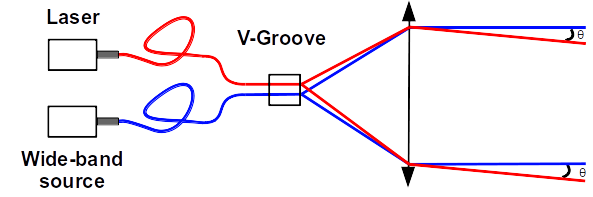
\includegraphics[width=0.95\textwidth]{Figure_Chap4/BinarySystemScheme_02.png}
        \caption{Schéma du système de source exoplanétaire avec, de la gauche vers la droite, la source large bande simulant le continuum et le laser simulant un compagnon, le V-Groove et une lentille convergente de $30 \,$cm de focale.}
        \label{fig:BinarySystA}
    \end{subfigure}
    \begin{subfigure}[t]{0.95\textwidth}
        \centering
        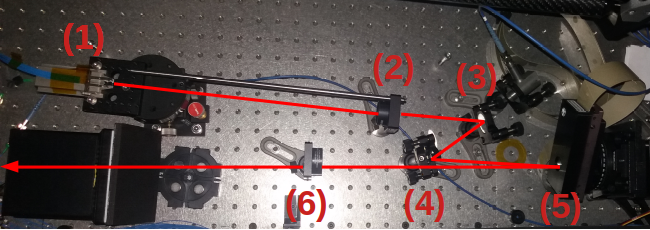
\includegraphics[width=\textwidth]{Figure_Chap4/20210531_BinarySetup_Crop_Annotation.png}
        \caption{Photo du simulateur de source exoplanétaire sur le banc de test de FIRSTv2. On y voit le V-Groove d'injection des sources (1) la lentille de collimation (2), le miroir plan de renvoi (3), le miroir en forme de D (4), le miroir MEMS (5) et la première lentille du système afocal (6).}
        \label{fig:BinarySystB}
    \end{subfigure}
    \caption[Simulateur du système protoplanétaire sur le banc de test de FIRSTv2 à Meudon.]{Simulateur du système protoplanétaire sur le banc de test de FIRSTv2 à Meudon.}
    \label{fig:BinarySyst}
\end{figure}

La figure~\ref{fig:BinarySystB} est une photo de ce montage installé sur le banc de test. On peut voir le V-Groove (1) et ses fibres bleues sur la gauche qui illuminent une lentille (2) au centre de l'image. Un premier miroir plan (3) renvoie le faisceau sur le miroir en forme de D (4) qui sert à illuminer le miroir segmenté (5) avec une incidence quasi-normale. La lentille (6) est la première lentille du doublet afocal d'agrandissement du faisceau (voir la section~\ref{sec:FiberInjection}) avant l'injection des faisceaux dans les fibres optiques vers la gauche de la photo.

\begin{figure}[ht!]
    \centering
    \begin{subfigure}{0.39\textwidth}
        \centering
        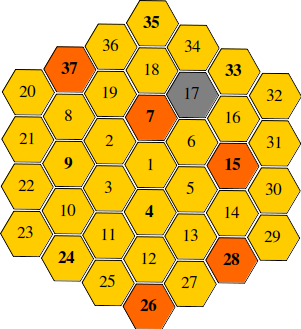
\includegraphics[width=\textwidth]{Figure_Chap2/BaselineMap_Meudon_37_7_26_15_28.png}
        \caption{Configuration des sous-pupilles choisies (en orange) dans le plan pupille sur la carte des segments du MEMS.}
        \label{fig:SegUVSimuleRappelA}
    \end{subfigure}\hfill
    \begin{subfigure}{0.59\textwidth}
        \centering
        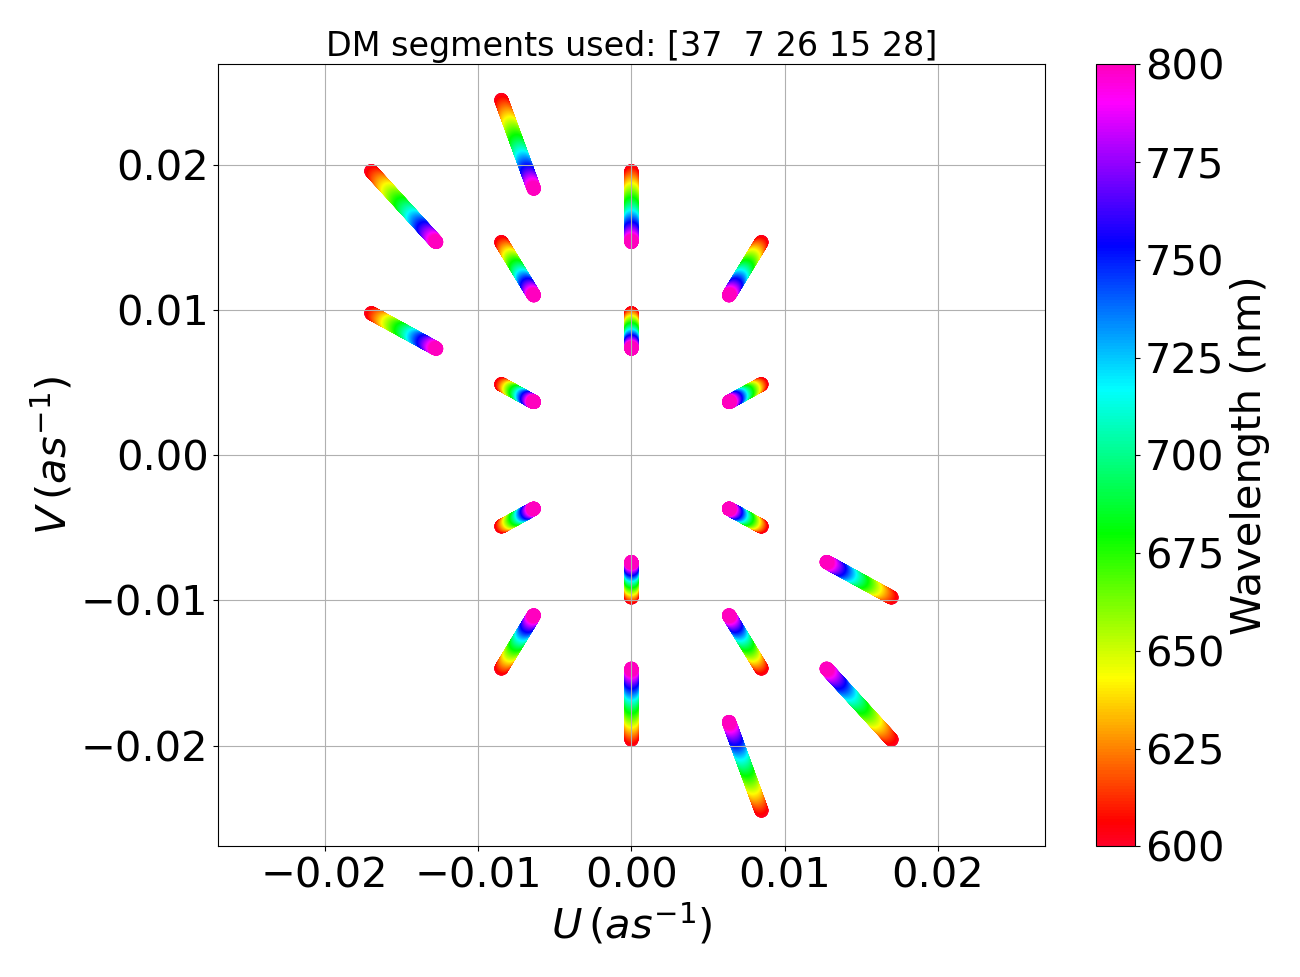
\includegraphics[width=\textwidth]{Figure_Chap2/UVplane_Meudon_37_7_26_15_28.png}
        \caption{La répartition des bases choisies représentée dans l'espace de Fourier, appelée aussi la couverture du plan UV des fréquences spatiales. Les couleurs représentent la longueur d'onde.}
        \label{fig:SegUVSimuleRappelB}
    \end{subfigure}
    \caption[Configuration des sous-pupilles et couverture du plan UV du banc de test de FIRSTv2.]{Configuration des sous-pupilles et couverture du plan UV du banc de test de FIRSTv2. Plus de détails sont présentés dans la section~\ref{sec:BaseConfig}.}
    \label{fig:SegUVSimuleRappel}
\end{figure}


%%%%%%%%%%%%%%%%%%%%%%%%%%%%%%%%
\section{L'analyse des phases différentielles sur une source protoplanétaire simulée}
\label{sec:PhaseDiffAnalyse}
%\kevinco{préciser sur quelle puce les phases sont mesurées, notamment si je ne présente les phases que d'une puce}

%%%%%%%%%%%%%%%%
\subsection{Les observables interférométriques sur un système protoplanétaire}

Pour comprendre et analyser les phases différentielles on souhaite exprimer la forme d'un tel signal de phase pour un système protoplanétaire tel que le système PDS 70. Pour commencer, la distribution d'intensité d'une telle source s'exprime comme :

\begin{equation}
    I = \frac{1}{1 + \rho(\lambda)} (\delta(\vv{r} - \vv{r_1}) + \rho(\lambda) \delta(\vv{r} - \vv{r_2}))
\end{equation}

avec $\vv{r} = (\alpha, \beta)$ le vecteur position angulaire, $\vv{r_1}$, $\vv{r_2}$ les positions de l'étoile et du compagnon respectivement, $\delta(\vv{r} - \vv{r_i})$ le pic de Dirac modélisant la source $i$ à la position $r_i$. Pour modéliser le contraste du système, j'utilise une fonction de Gauss centrée sur la longueur d'onde $\lambda_c$ du pic d'émission du compagnon et d'écart-type $\sigma_c$ de la façon suivante : 

\begin{equation}
    \rho(\lambda) = \rho_{\lambda_c} e^{\frac{-(\lambda - \lambda_c)^2}{2 \sigma_{c}^2}}
\end{equation}

où $\rho_{\lambda_c}$ est le contraste du système à la longueur d'onde $\lambda_c$. La visibilité complexe associée à une telle source s'écrit alors :

\begin{equation}
    V = \frac{e^{2i\pi \vv{r_1} \cdot \vv{f}}}{1 + \rho(\lambda)} \left( 1 + \rho(\lambda) e^{2i\pi \vv{\Theta} \cdot \vv{f}} \right)
\end{equation}

avec $\vv{\Theta} = \vv{r_2} - \vv{r_1}$ la séparation angulaire des deux composantes du système et $\vv{f} = \vv{B} / \lambda$ le vecteur fréquence spatiale. $\vv{B}$ est le vecteur de base formé par deux sous-pupilles. On en déduit ainsi la phase comme suit :

\begin{equation}
    \varphi = atan \left( \frac{sin(2\pi \vv{r_1} \cdot \vv{f}) + \rho(\lambda) sin(2\pi \vv{r_2} \cdot \vv{f})}{cos(2\pi \vv{r_1} \cdot \vv{f}) + \rho(\lambda) cos(2\pi \vv{r_2} \cdot \vv{f})} \right) \label{eq:PhaseBinaire}
\end{equation}

La phase dépend donc de la position de la source par rapport au point centré par le télescope. Nous considérons donc que le télescope pointe sur l'étoile centrale, i.e. $\vv{r_1} = (0, 0)$ nous permettant de simplifier l'équation~\ref{eq:PhaseBinaire} comme suit :

\begin{equation}
    \varphi = atan \left( \frac{\rho(\lambda) sin(2\pi \vv{\Theta} \cdot \vv{f})}{1 + \rho(\lambda) cos(2\pi \vv{\Theta} \cdot \vv{f})} \right) \label{eq:PhaseBinaireCentree}
\end{equation}

De plus, pour un système avec un haut contraste telle que les systèmes exoplanétaires, i.e. $\rho(\lambda) \ll 1$, l'équation~\ref{eq:PhaseBinaireCentree} s'approxime de la manière suivante :

\begin{equation}
    \varphi \approx \rho(\lambda) sin(2\pi \vv{\Theta} \cdot \vv{f})
    \label{eq:PhaseBinaireHautContraste}
\end{equation}


%%%%%%%%%%%%%%%%
\subsection{Le modèle des signaux de phase différentielle pour un système protoplanétaire}

Le signal de phase différentielle mesuré par un interféromètre dépend des bases (de leur longueur et de leur orientation) mais aussi de la séparation entre les deux composantes de la source observée. Pour illustrer ce propos, le signal de phase attendu, d'après l'équation~\ref{eq:PhaseBinaireCentree}, pour les bases présentées précédemment, est tracé en fonction de la séparation entre l'étoile et le compagnon pour un contraste de luminosité égal à $1$ sur la figure~\ref{fig:PhaseDiffBinSizeSimuleA}, à $0,1$ sur la figure~\ref{fig:PhaseDiffBinSizeSimuleB} et à $0,01$ sur la figure~\ref{fig:PhaseDiffBinSizeSimuleC}. On retrouve les trois amplitudes de phase correspondant aux trois groupes de bases identifiés dans la section~\ref{sec:BaseConfig} avec celle qui est nulle quelle que soit la séparation (correspondant aux bases orthogonales au système protoplanétaire). De plus, comme l'indique l'équation~\ref{eq:PhaseBinaireHautContraste}, la phase est sinusoïdale pour des hauts contrastes ($< 0,1$), avec une amplitude égale à ce contraste, ici $0,1 \, \text{rad} = 5,7\degree$ et $0,01 \, \text{rad} = 0,57\degree$, comme attendu, pour les figures~\ref{fig:PhaseDiffBinSizeSimuleB} et \ref{fig:PhaseDiffBinSizeSimuleC}, respectivement. Par conséquent, plus le système protoplanétaire présente un contraste élevé, plus le signal de phase attendu est faible et plus le compagnon est difficile à détecter. Les systèmes protoplanétaires qui présentent un contraste plus faible dans la raie d'émission \ha~sont donc particulièrement intéressants car le signal de phase à détecter est de plus forte amplitude.

\begin{figure}[ht!]
    \centering
    \begin{subfigure}{0.5\textwidth}
        \centering
        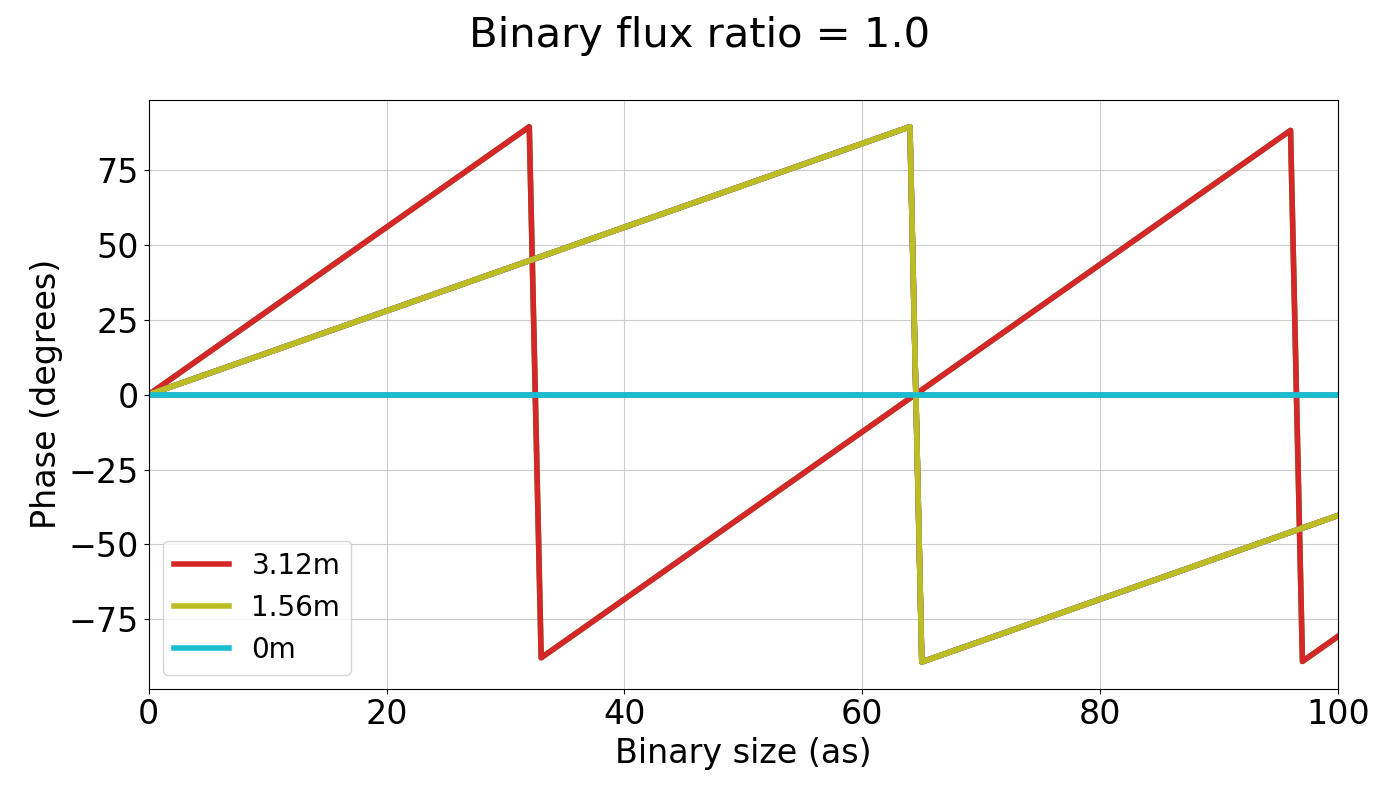
\includegraphics[width=\textwidth]{Figure_Chap4/SpectralDiffPhase_VS_BinSize_FR1e0_37_7_26_15_28.png}
        \caption{}
        \label{fig:PhaseDiffBinSizeSimuleA}
    \end{subfigure}
    \begin{subfigure}{0.5\textwidth}
        \centering
        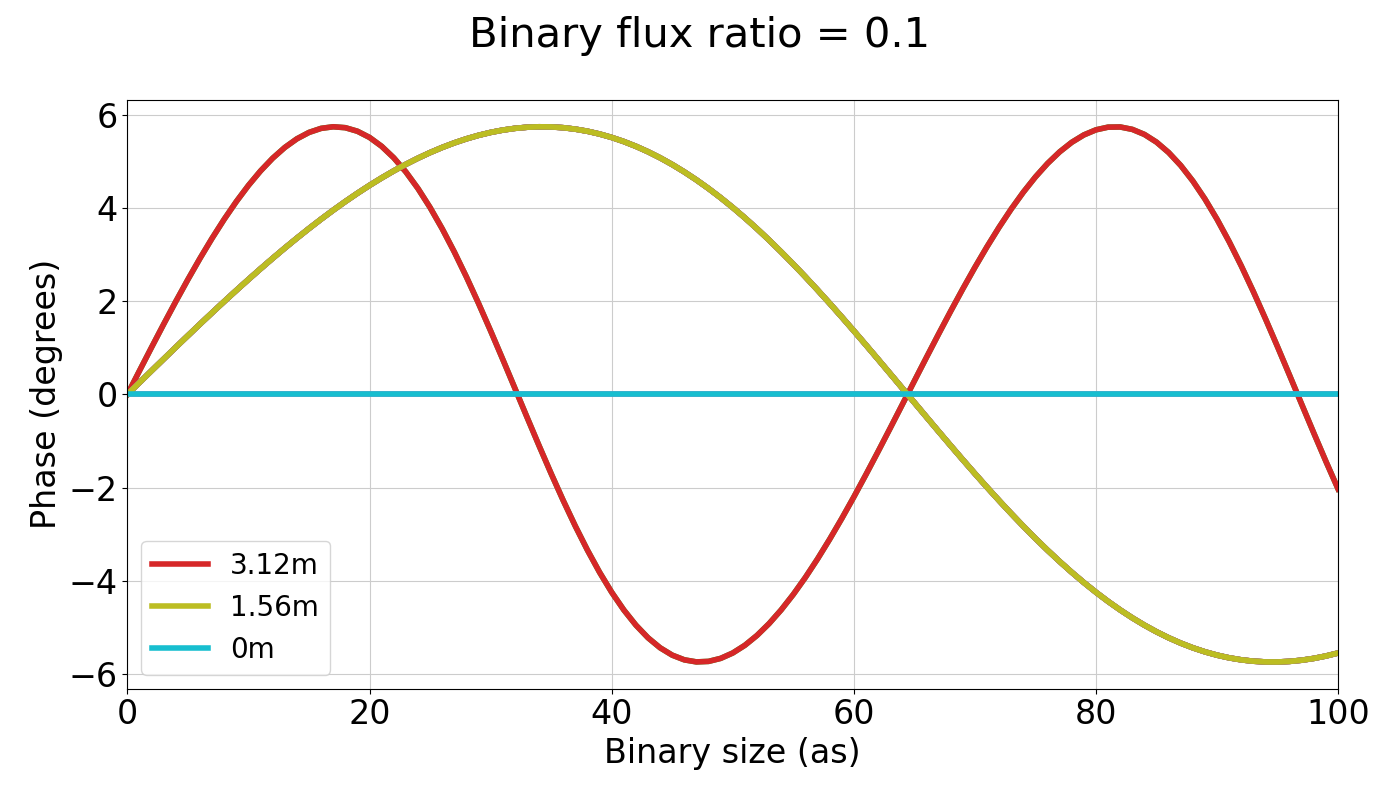
\includegraphics[width=\textwidth]{Figure_Chap4/SpectralDiffPhase_VS_BinSize_FR1e-1_37_7_26_15_28.png}
        \caption{}
        \label{fig:PhaseDiffBinSizeSimuleB}
    \end{subfigure}%
    \begin{subfigure}{0.5\textwidth}
        \centering
        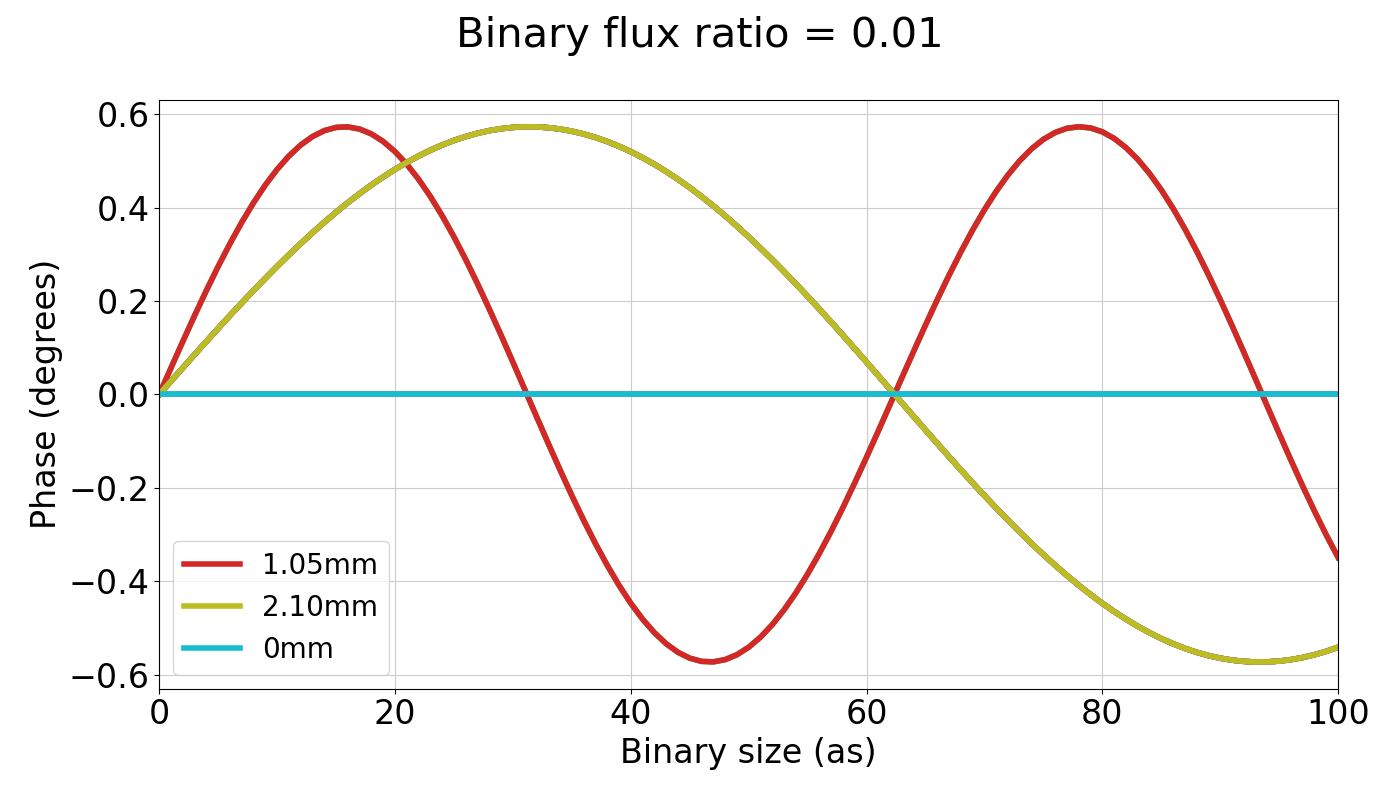
\includegraphics[width=\textwidth]{Figure_Chap4/SpectralDiffPhase_VS_BinSize_FR1e-2_37_7_26_15_28.png}
        \caption{}
        \label{fig:PhaseDiffBinSizeSimuleC}
    \end{subfigure}
    \caption[Courbes de phases théoriques en fonction de la séparation du système observé.]{Courbes de phases théoriques en fonction de la séparation du système observé pour des contrastes de $1$ \textit{(a)}, $0,1$ \textit{(b)} et $0,01$ \textit{(c)} et pour la longueur d'onde $635 \,$nm.}
    \label{fig:PhaseDiffBinSizeSimule}
\end{figure}

Mais encore, l'équation~\ref{eq:PhaseBinaireHautContraste} nous renseigne sur les séparations pour lesquelles les signaux de toutes les bases sont nuls (possible ici car la longueur de la plus grande base est le double de la longueur de la plus petite) : i.e. pour $2\pi \vv{\Theta} \cdot \vv{f} = \pi [\pi]$ soit une séparation valant $\text{k} \lambda / 2B$ avec k un entier relatif. Ce qui donne pour B, la longueur de la base la plus grande, pour la longueur d'onde du laser simulant la protoplanète sur le banc de test $\uplambda = 635 \,$nm, ainsi que pour $\text{k} \in \llbracket 0; 3 \rrbracket$, les séparations $0 \,$as, $31,2 \,$as, $62,4 \,$as et $93,6 \,$as. En revanche, le signal de phase est maximal lorsque $2\pi \vv{\Theta} \cdot \vv{f} = \pi / 2 [\pi]$, i.e. pour une séparation valant : $(2\text{k}+1) \lambda / 4B$. De même, pour la plus grande longueur de base B et pour $\text{k} \in \llbracket 0; 3 \rrbracket$, les séparations qui induisent un signal de phase maximal sont $16,1 \,$as, $48,3 \,$as, $80,5 \,$as et $113 \,$as. Pour l'autre longueur de base la séparation égale à $96,6 \,$as maximise le signal. La séparation choisie sur le banc de test, égale à $87,3 \,$as (voir la section~\ref{sec:SystBinaire}) est un bon compromis entre les séparations $80,5 \,$as et $96,6 \,$as, pour maximiser le signal de phase sur toutes les bases et tout en utilisant le matériel qui était à disposition pour simuler la source protoplanétaire (le V-Groove et la lentille).

A présent, pour la séparation choisie, les phases différentielles sont simulées en fonction de la longueur d'onde et sont présentées pour un contraste de la source égal à $1$ sur la figure~\ref{fig:PhaseDiffWaveSimuleA}, à $0,1$ sur la figure~\ref{fig:PhaseDiffWaveSimuleB} et à $0,01$ sur la figure~\ref{fig:PhaseDiffWaveSimuleC}. Dans ces simulations, le compagnon présente une raie d'émission à $656 \,$nm (raie \ha), avec une largeur à mi-hauteur égale à $0,4 \,$nm, donnant à cette longueur d'onde les contrastes cités. Cette largeur est prise pour correspondre à la largeur de bande du laser qu'on utilise sur le banc de test, comme mesuré dans la section~\ref{sec:PhaseDiffMesure}. La résolution spectrale a été fixée à $3\,200$ ce qui correspond à la résolution spectrale de \ac{FIRSTv2} (mesurée et présentée dans la section~\ref{sec:EtalonnageSpectral}).

\begin{figure}[ht!]
    \centering
    \begin{subfigure}{0.5\textwidth}
        \centering
        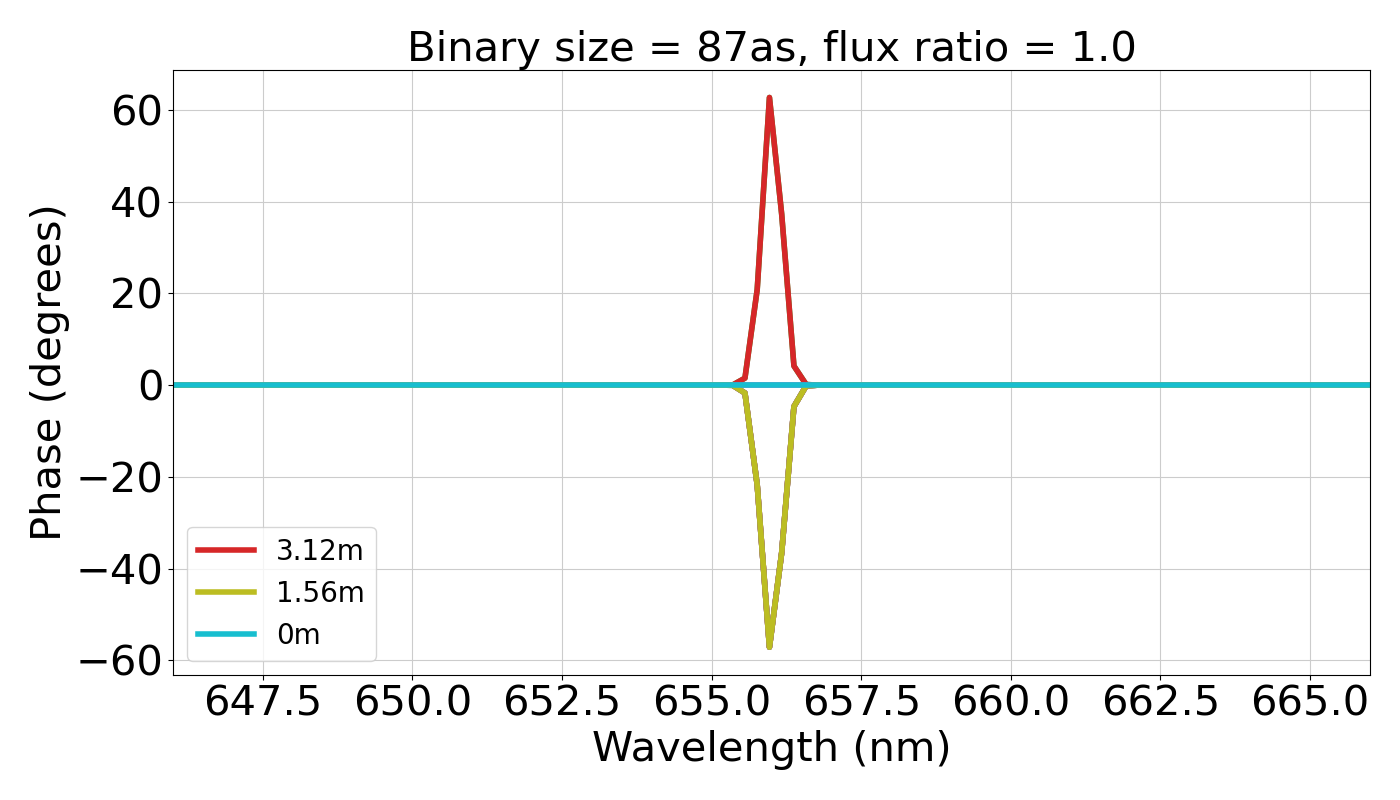
\includegraphics[width=\textwidth]{Figure_Chap4/SpectralDiffPhase_BinSize87_FR1e0_37_7_26_15_28_SpecRes3200.png}
        \caption{}
        \label{fig:PhaseDiffWaveSimuleA}
    \end{subfigure}
    \begin{subfigure}{0.5\textwidth}
        \centering
        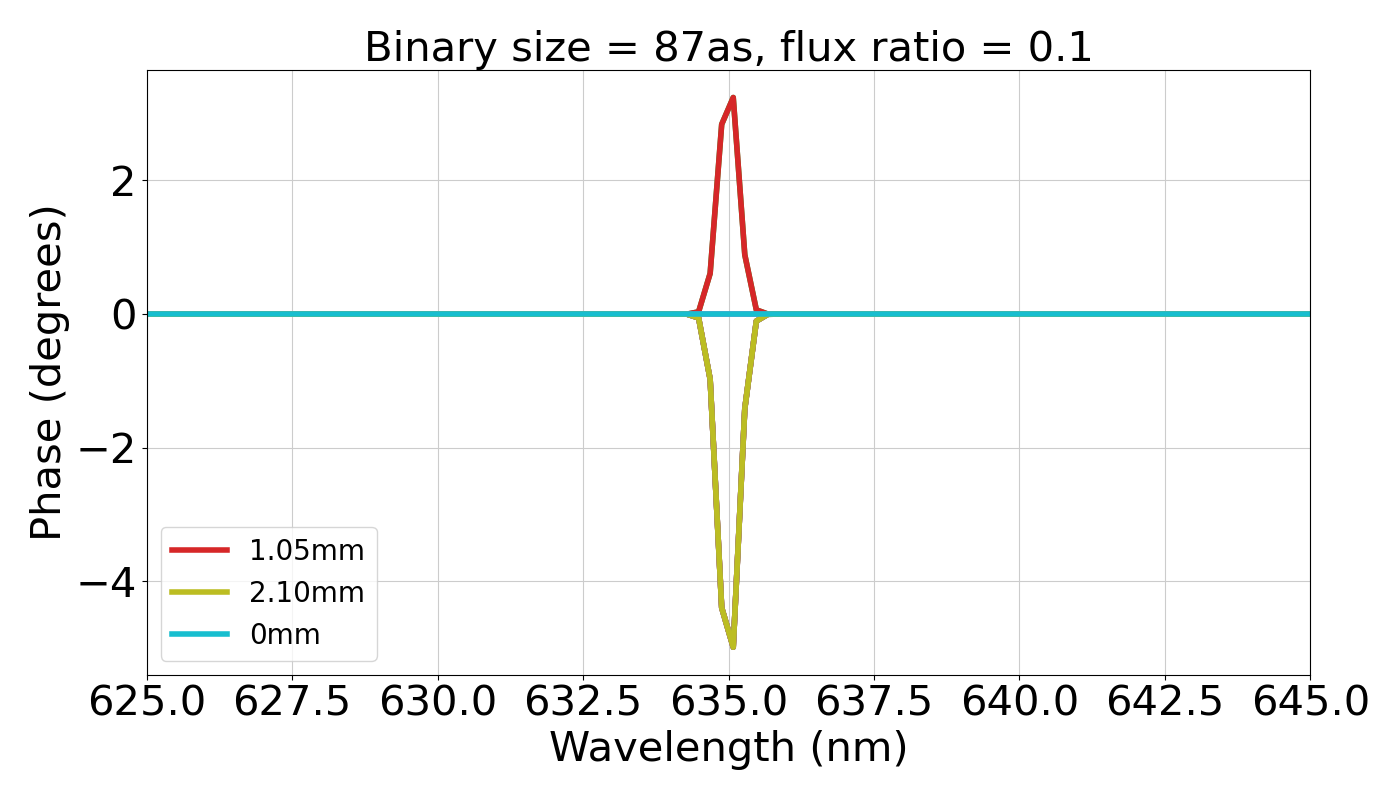
\includegraphics[width=\textwidth]{Figure_Chap4/SpectralDiffPhase_BinSize87_FR1e-1_37_7_26_15_28_SpecRes3200.png}
        \caption{}
        \label{fig:PhaseDiffWaveSimuleB}
    \end{subfigure}%
    \begin{subfigure}{0.5\textwidth}
        \centering
        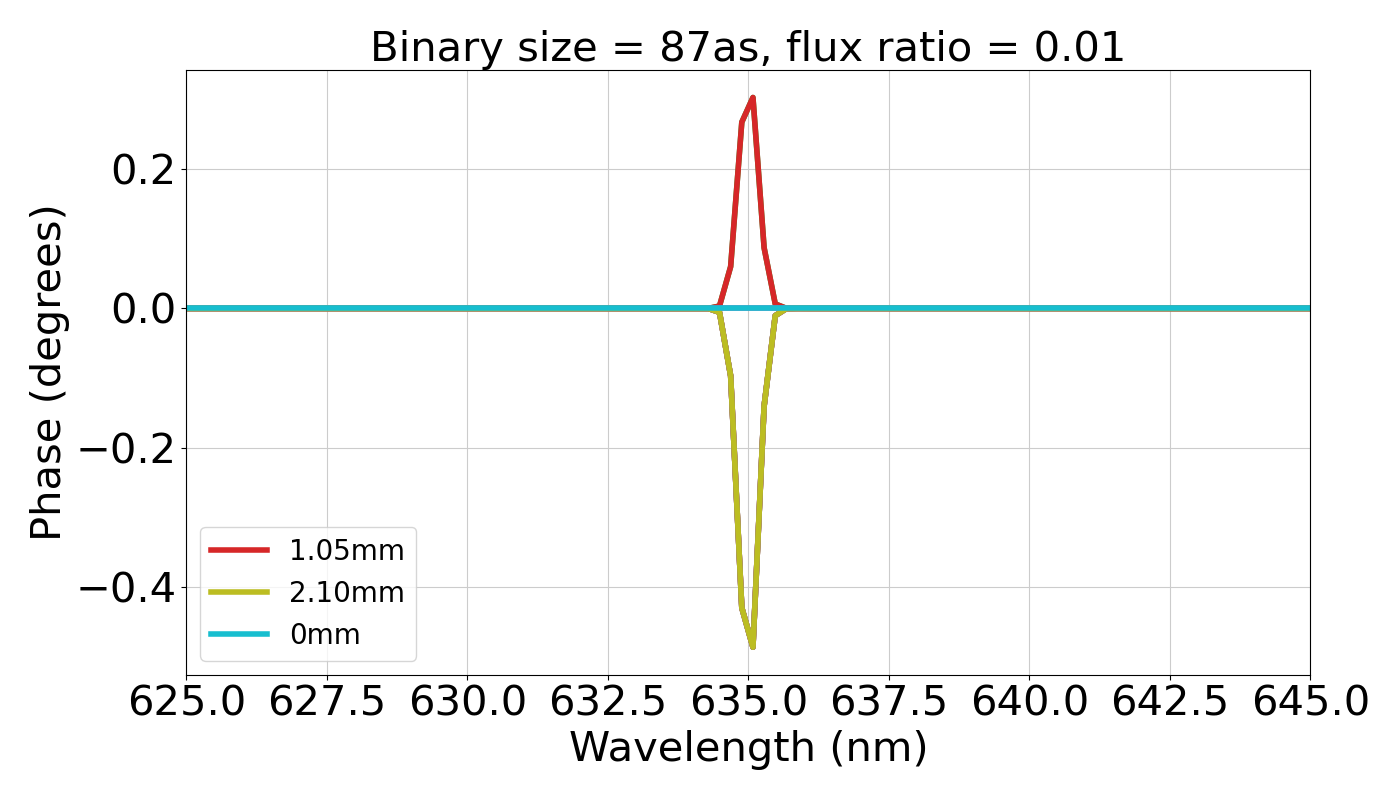
\includegraphics[width=\textwidth]{Figure_Chap4/SpectralDiffPhase_BinSize87_FR1e-2_37_7_26_15_28_SpecRes3200.png}
        \caption{}
        \label{fig:PhaseDiffWaveSimuleC}
    \end{subfigure}
    \caption[Courbes de phases théoriques en fonction de la longueur d'onde pour plusieurs contrastes.]{Courbes de phases théoriques en fonction de la longueur d'onde pour les contrastes de $1$ \textit{(a)}, de $0,1$ \textit{(b)} et de $0,01$ \textit{(c)}. Le compagnon a été simulé avec une raie d'émission à $656 \,$nm, de largeur à mi-hauteur de $0,4 \,$nm et une résolution spectrale de $3\,200$.}
    \label{fig:PhaseDiffWaveSimule}
\end{figure}

Je me servirai de ce modèle pour ajuster les courbes de phases mesurées par la suite afin d'inférer le contraste du système et la séparation du compagnon. Pour cela, on souhaite ajuster aux mesures de phases différentielles, le modèle de la phase d'un système protoplanétaire en accrétion exprimé par l'équation~\ref{eq:PhaseBinaireCentree}. Pour ce faire, on souhaite minimiser la fonction $\chi^2$ définie comme suit :

\begin{equation}
    \chi^2 (\rho, \alpha, \beta) = \sum_{k}^{n_B} \frac{(\varphi_{k, mesure} - \varphi_{k, modele})^2}{\sigma^{k^2}}
    \label{eq:chi2}
\end{equation}

\noindent avec $\varphi_{k, mesure}$ l'estimation du terme de phase de la base $k$, $\varphi_{k, modele}$ le terme de phase du modèle de la base $k$, $\sigma^{k}$ l'erreur sur la mesure du terme de phase de la base $k$ et $n_B$ le nombre de bases. L'erreur $\sigma^{k}$ est estimée à partir de l'écart-type de la phase sur une centaine de canaux spectraux autour du pic d'émission du compagnon (voir ces mesures dans la section~\ref{sec:PhaseDiffMesure}). Cette minimisation est conduite sur des intervalles de contraste du système $\rho$ et des positions $(\alpha, \beta)$ qui sont les coordonnées du vecteur de séparation angulaire $\vv{\Theta}$ afin de trouver les valeurs optimales pour la longueur d'onde du pic du signal de la protoplanète.

Ensuite, à partir de la fonction $\chi^2$, on en déduit la fonction de vraisemblance suivante :

\begin{equation}
    \Like (\rho, \alpha, \beta) \propto e^{\frac{-\chi^2 (\rho, \alpha, \beta)}{2}}
\end{equation}

Chacun des trois paramètres est alors estimé par la marginalisation de la fonction de vraisemblance $\Like (\rho, \alpha, \beta)$ sur les deux autres paramètres, par exemple, selon l'expression suivante pour le paramètre $\rho$ :

\begin{equation}
    f (\rho) \propto \int_{\alpha} \int_{\beta} \Like (\rho, \alpha, \beta) d\alpha d\beta
\end{equation}

La loi de densité est obtenue après avoir normalisé numériquement cette expression et la valeur la plus probable du paramètre associé est estimée par la médiane de cette loi. Enfin, l'intervalle de confiance sur l'estimation du paramètre est pris à $68 \%$ de probabilité autour de la médiane.


%%%%%%%%%%%%%%%%
\subsection{Les phases différentielles mesurées sur une source non résolue}

Dans un premier temps, je vais présenter les mesures de phases différentielles sur une source non résolue par l'instrument. Sur le banc de test, c'est la source qui simule l'étoile centrale : la source fibrée Leukos-SM8-OEM ou super continuum (dénommé par la suite \sk), fabriquée par \textit{Leukos}\footnote{\url{https://www.leukos-laser.com/}} et qui est lumineuse sur la large bande $400 - 2\,400 \,$nm. La source est injectée dans une fibre optique PM630-HP fabriquée par \textit{Thorlabs}\footnote{\url{https://www.thorlabs.com/}} avec un \ac{MFD} égal à $4,5 \pm 0,5 \,$\um, correspondant à une taille angulaire de la source vue par le reste du banc égale à $3,1 \,$as, soit une taille angulaire de $\sim 0,05 \lambda / \text{B}$ (avec $\text{B} = 2,1 \,$mm, la longueur de la plus grande base). La figure~\ref{fig:SuperKSpectrum} montre l'intensité lumineuse normalisée de la \sk~mesurée par \ac{FIRSTv2} en fonction de la longueur d'onde, qui a une forme qui dépend de la transmission du banc. On note que le spectre présente des oscillations à hautes fréquences, qu'on appellera \wiggles~par la suite. Comme nous le verrons, ces oscillations sont problématiques pour les mesures de phases, je présenterai leur caractérisation dans la section~\ref{sec:wiggles}.

\begin{figure}[ht!]
    \centering
    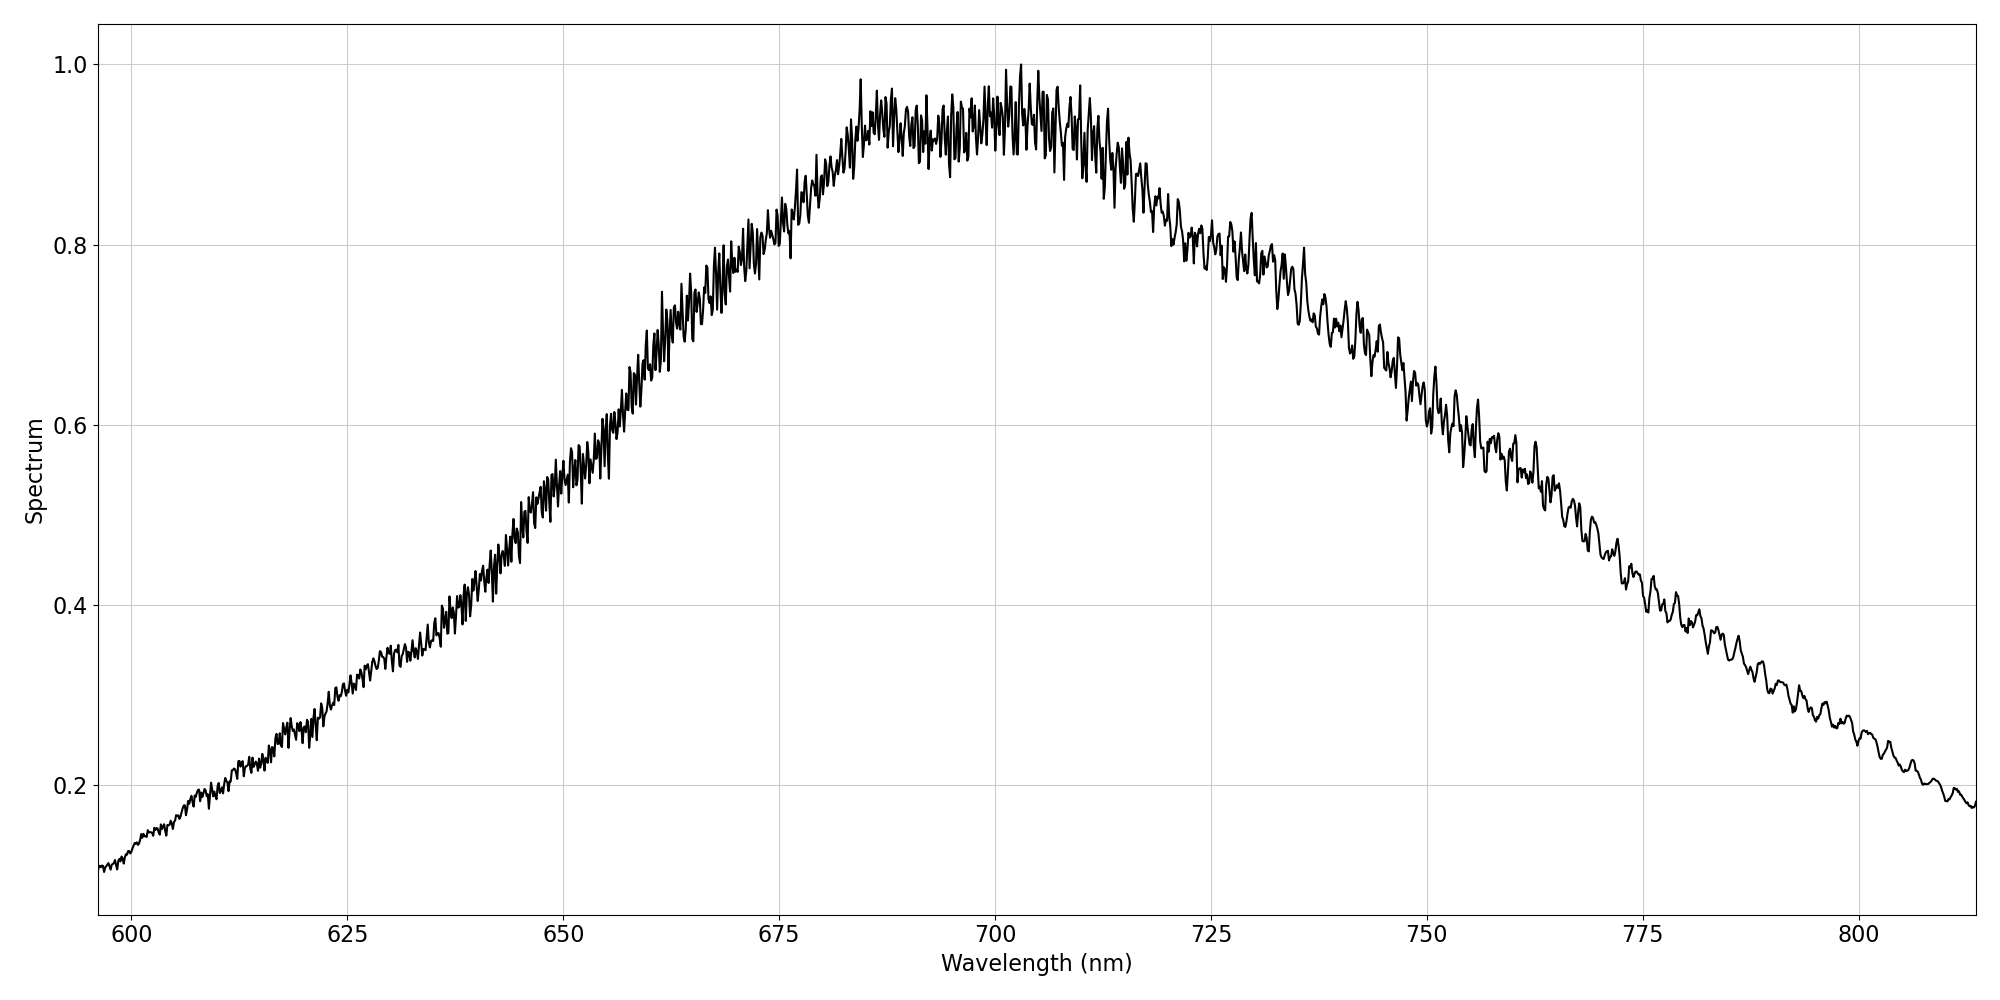
\includegraphics[width=\figwidth]{Figure_Chap4/20221010_Bin01_Spectra_superK_Pola1_LaTex.png}
    \caption[Intensité lumineuse en fonction de la longueur d'onde de la source de référence (\sk) mesurée par FIRSTv2.]{Intensité lumineuse en fonction de la longueur d'onde de la source \sk~de référence, simulant l'étoile centrale du système protoplanétaire, mesurée par FIRSTv2, entre $600 \,$nm et $810 \,$nm.}
    \label{fig:SuperKSpectrum}
\end{figure}

Les phases différentielles mesurées pour les dix bases sur la source \sk, selon la méthode décrite dans la section~\ref{sec:PhaseSpecDiff}, sont tracées sur le graphique de la figure~\ref{fig:PhaseDiffSuperK}. Le signal de phase différentielle sur une source unique non résolue est attendu nul. Or ici nous remarquons 1- des oscillations hautes fréquences qui font penser aux \wiggles~précédemment vus sur le spectre de la source; 2- des oscillations plus basses fréquences qui ressemblent aux spectres de transmissions relatives des puces présentés sur la figure~\ref{fig:V2PMtransmission}.

\begin{figure}[ht!]
    \centering
    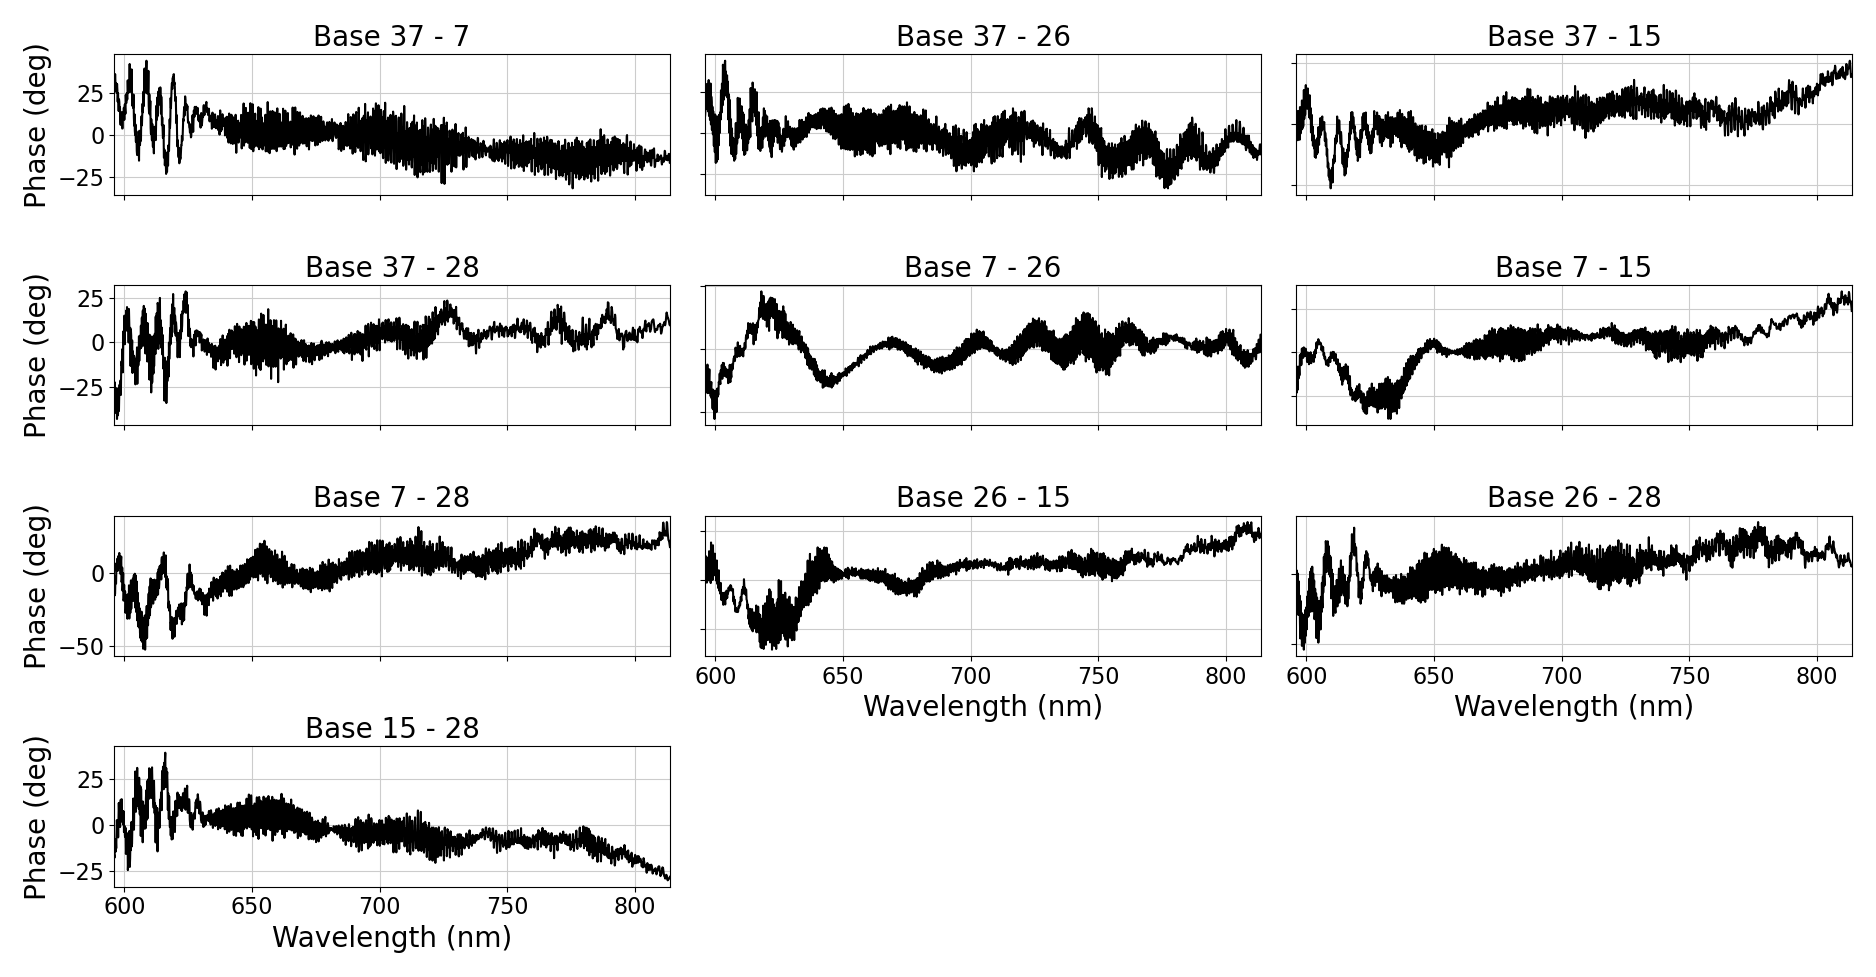
\includegraphics[width=\figwidth]{Figure_Chap4/20221010_SpeDiffPhase_BaseSubplot_Pola1_LaTex.png}
    \caption[Phases différentielles mesurées sur la source \sk~de référence simulant l'étoile centrale.]{Phases différentielles mesurées sur la source \sk~de référence simulant l'étoile centrale, pour les dix bases de FIRSTv2. Les mesures sont présentées en fonction de la longueur d'onde entre $620 \,$nm et $660 \,$nm.}
    \label{fig:PhaseDiffSuperK}
\end{figure}

Les mesures de phases subissent donc les effets indésirables de phénomènes instrumentaux. La phase différentielle est une grandeur auto-étalonnée des termes instrumentaux qui ont une dépendance polynomiale en fonction de la longueur d'onde. Les perturbations telles que les \wiggles~ne sont donc pas étalonnées. C'est pour cette raison que je vais chercher à les corriger sur les phases différentielles de la source protoplanétaire par la soustraction des phases différentielles de la source non résolue.


%%%%%%%%%%%%%%%%
\subsection{Mesure et étalonnage des phases différentielles sur une source protoplanétaire simulée}
\label{sec:PhaseDiffMesure}

Les résultats préliminaires portant sur les mesures que je vais présenter ici ont été présentés dans la conférence \cite{barjot2022} (voir la section~\ref{sec:HypatiaProceeding}). Dans cette partie je vais exposer les mesures des phases différentielles sur la source protoplanétaire simulée sur le banc de test. Pour cela, la source simulant l'étoile centrale est la source de référence décrite dans la partie précédente et la source simulant une protoplanète en accrétion est un laser fibré, à $635 \,$nm, fabriqué par \textit{Thorlabs}. La figure~\ref{fig:BinarySpectrum} montre l'intensité lumineuse en fonction de la longueur d'onde de la source protoplanétaire simulée, mesurée par \ac{FIRSTv2}. Le graphique est une superposition de l'intensité de l'étoile centrale en trait discontinu et de l'intensité de la source du système (étoile + protoplanète) en trait plein, normalisées par l'intensité de la source centrale à $635 \,$nm, où est visible le pic du laser. La largeur spectrale (largeur à mi-hauteur) du laser est mesurée à $\sim 0,4 \,$nm. À l'aide de ces courbes, une première estimation du rapport de flux entre les deux composantes est faite à $\sim 0,39$. Je règle grossièrement ce contraste lumineux entre les deux sources en desserrant le connecteur de la fibre optique de la source laser.

\begin{figure}[ht!]
    \centering
    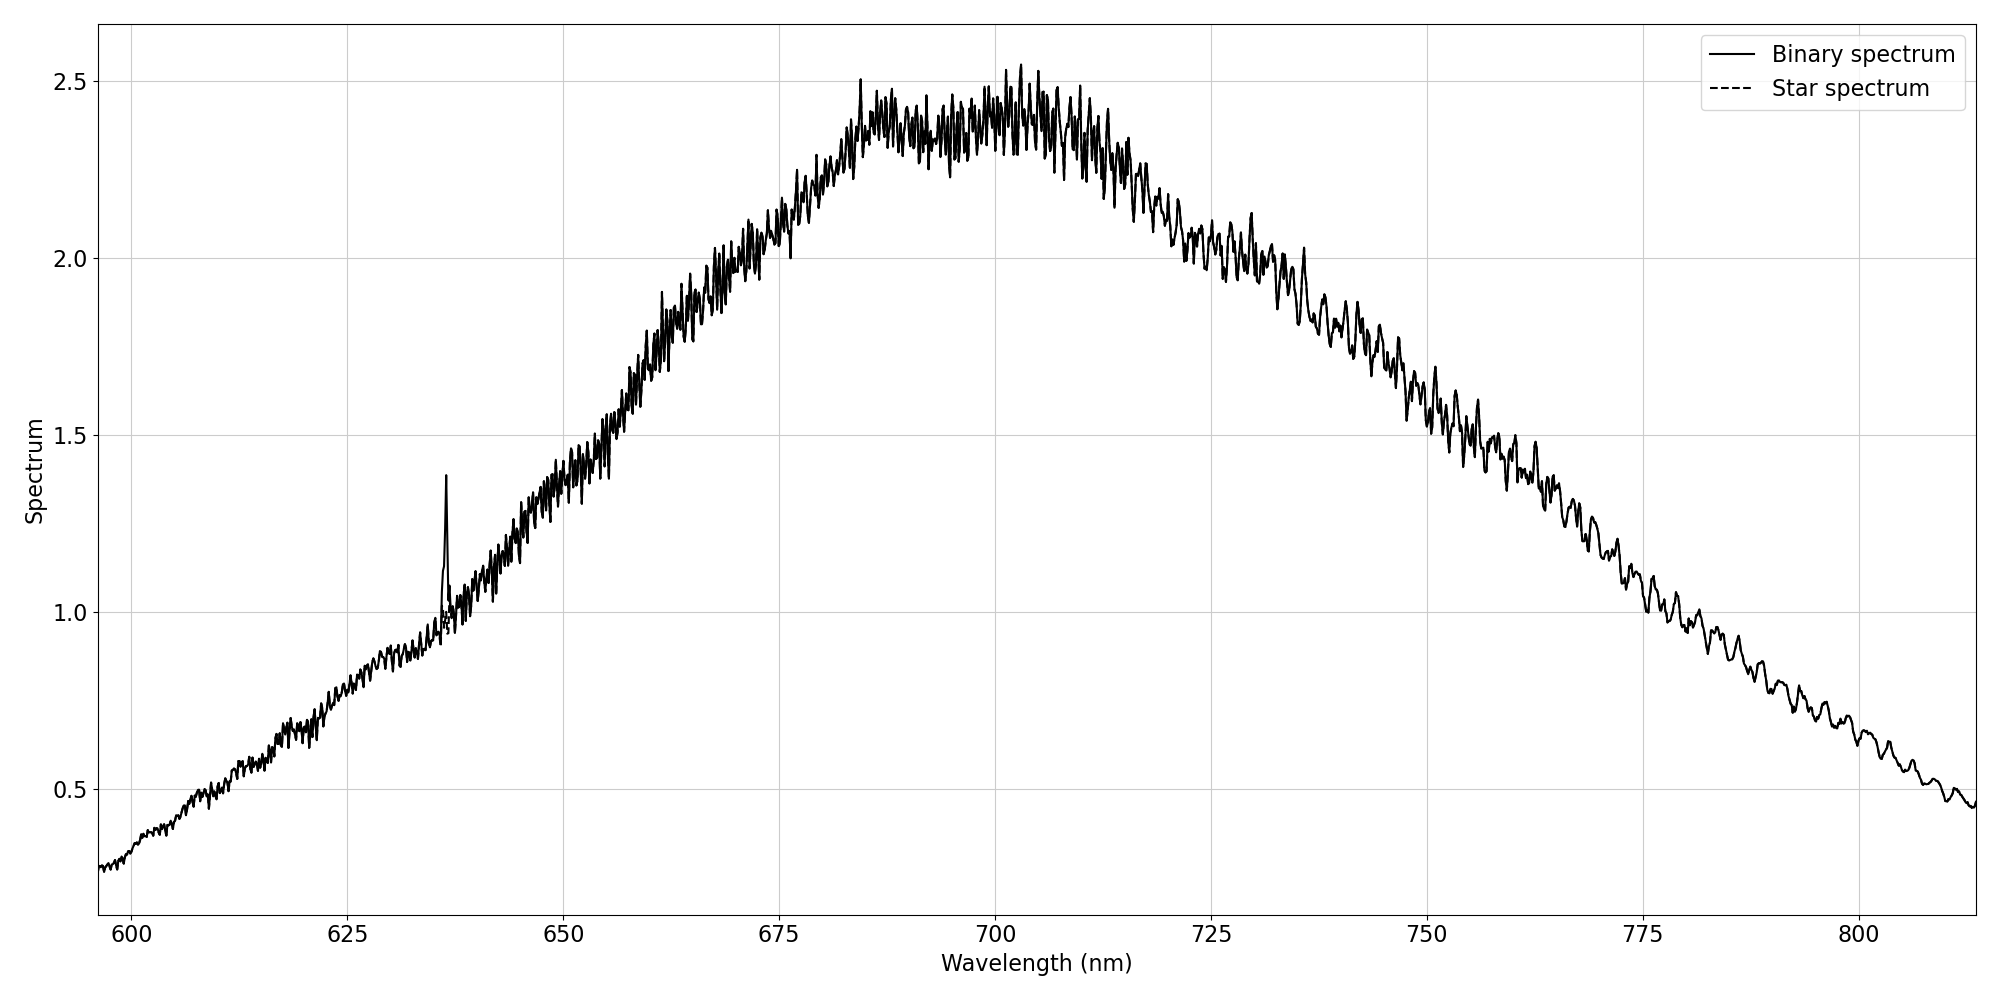
\includegraphics[width=\figwidth]{Figure_Chap4/20221010_Bin01_Spectra_superK_laser635_Pola1_LaTex.png}
    \caption[Intensité lumineuse en fonction de la longueur d'onde de la source protoplanétaire mesurée par FIRSTv2.]{Intensité lumineuse en fonction de la longueur d'onde de la source protoplanétaire mesurée par FIRSTv2, entre $600 \,$nm et $810 \,$nm. L'intensité de l'étoile seule est tracée en trait discontinu et l'intensité du système total (étoile + protoplanète) est tracée en trait plein. Les deux courbes sont normalisées par l'intensité de l'étoile à $635 \,$nm, où est visible le pic du laser et le rapport de flux entre les deux composantes (à cette longueur d'onde) est estimé à $\sim 0,39$.}
    \label{fig:BinarySpectrum}
\end{figure}

Les phases différentielles mesurées sur cette source, avant étalonnage par la source centrale, sont tracées sur les graphiques du haut de la figure~\ref{fig:PhaseDiffBinary}. On remarque la présence d'un pic de phase à $\sim 636 \,$nm, correspondant à l'émission du compagnon. De plus, on retrouve les mêmes perturbations instrumentales hautes fréquences qui étaient observées sur la figure~\ref{fig:PhaseDiffSuperK} des phases mesurées sur l'étoile seule. Les courbes sont la moyenne de quelques dizaines de mesures de courbe de phase et les barres d'erreur (très petites sur ces graphiques) sont estimées à partir de leur écart-type. De plus, on estime l'erreur induite par les \wiggles~sur la mesure de la phase différentielle à la longueur d'onde du pic d'émission en calculant l'écart-type $\sigma_{\lambda}$ sur une centaine de canaux spectraux de la phase autour du pic du signal de la protoplanète (le pic étant exclu), pour chaque base. Cet écart-type est indiqué dans les sous-titres au-dessus de chaque graphique et il est en moyenne égal à $8 \pm 2\degree$. De plus, on note, qualitativement, que ces perturbations sont de même amplitude, voire de plus grande amplitude pour certaines bases ($7-15$, $7-28$, $26-15$ et $26-28$), que le signal associé au compagnon, il est donc important qu'on puisse les corriger.

Avant toute chose, il faut préciser que le laser utilisé pour simuler le compagnon n'est pas stable en longueur d'onde et celle-ci varie aléatoirement sur une bande spectrale d'environ $0,6 \,$nm de largeur (ce qui correspond à environ cinq pixels de la caméra). Par conséquent, le pic du signal du compagnon se décale d'autant de pixels de manière aléatoire au fil des mesures temporelles des phases. Une première solution est d'appliquer un \textit{binning} spectral afin de sommer la valeur des pixels par paquet de $5$. J'ai préféré abandonner cette méthode car l'effet de moyenne dégrade la résolution spectrale et diminue l'amplitude du signal qu'on souhaite mesurer. Une deuxième solution, que je préfère utiliser et qui est celle montrée ici, est de sélectionner pour chaque base, un ensemble des courbes de phase pour lesquelles le pic du signal est mesuré sur un même pixel. En pratique, cela correspond à garder environ $60\%$ des données. Ensuite, ces phases différentielles sélectionnées sont moyennées avant d'être étalonnées.

\begin{figure}[ht!]
    \centering
    \begin{subfigure}{\textwidth}
        \centering
        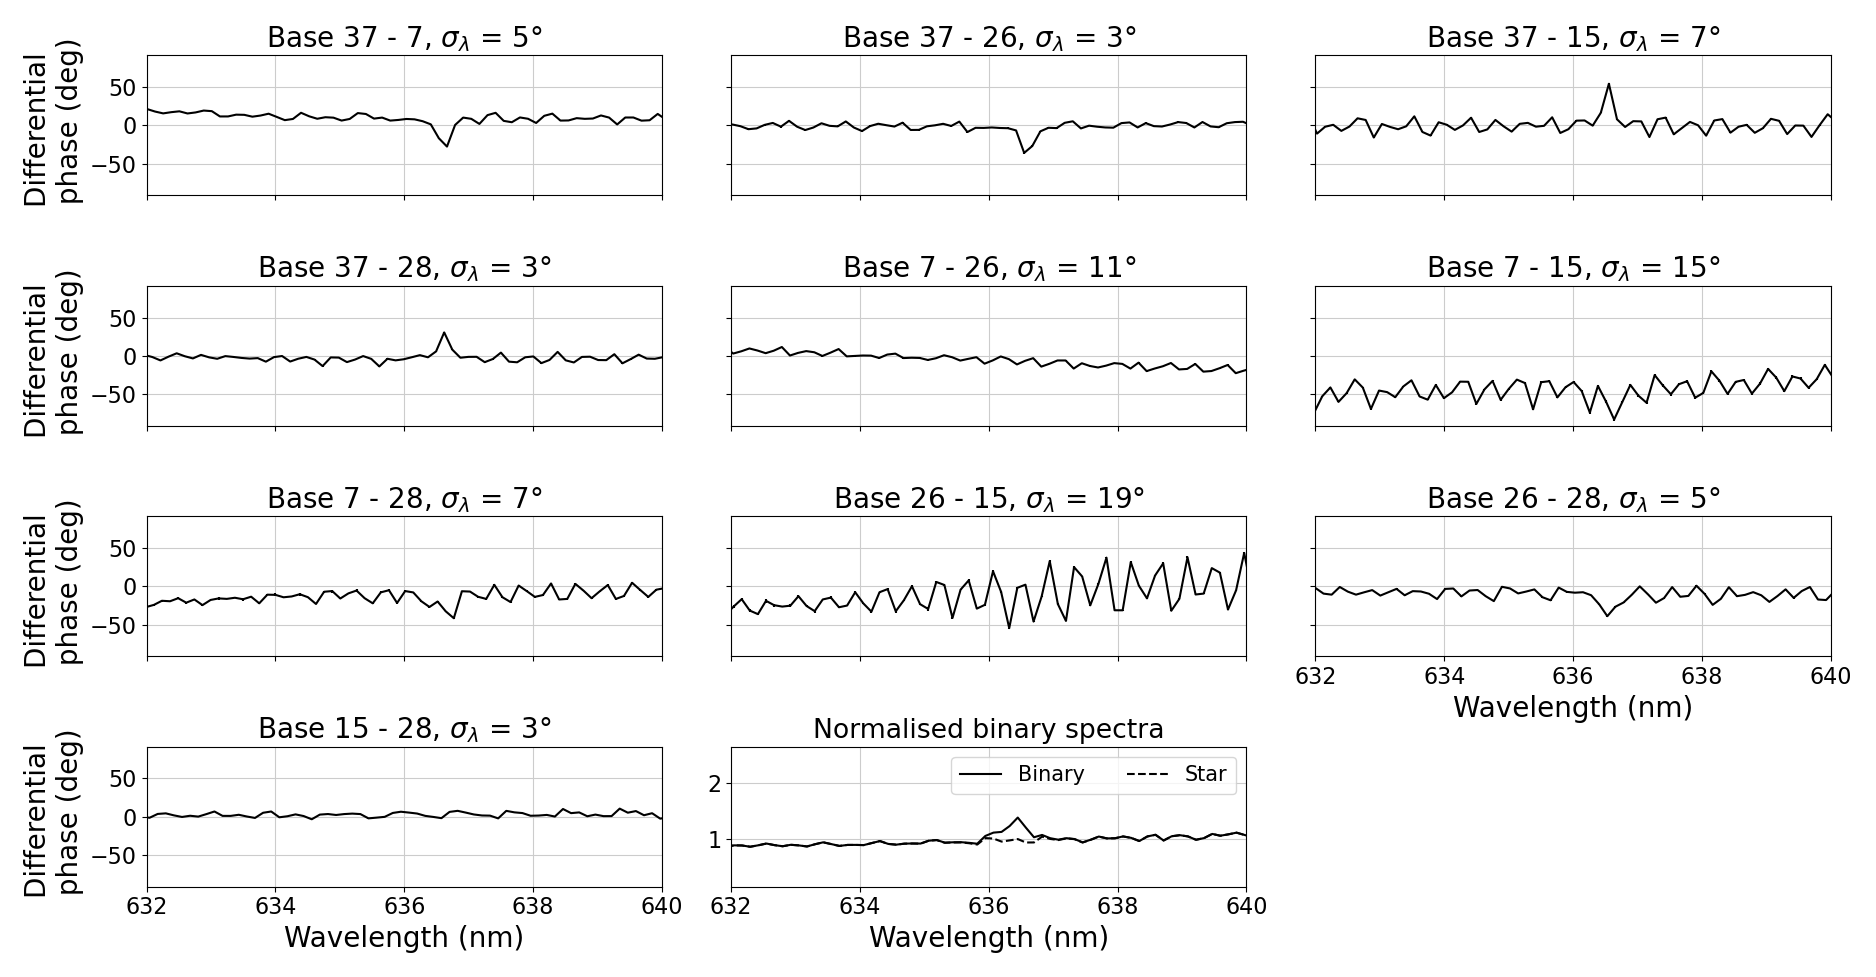
\includegraphics[width=\textwidth]{Figure_Chap4/20221010_Bin01_SpeDiffPhase_Raw_BaseSubplot_Pola1_LaTex.png}
    \end{subfigure}
    \begin{subfigure}{\textwidth}
        \centering
        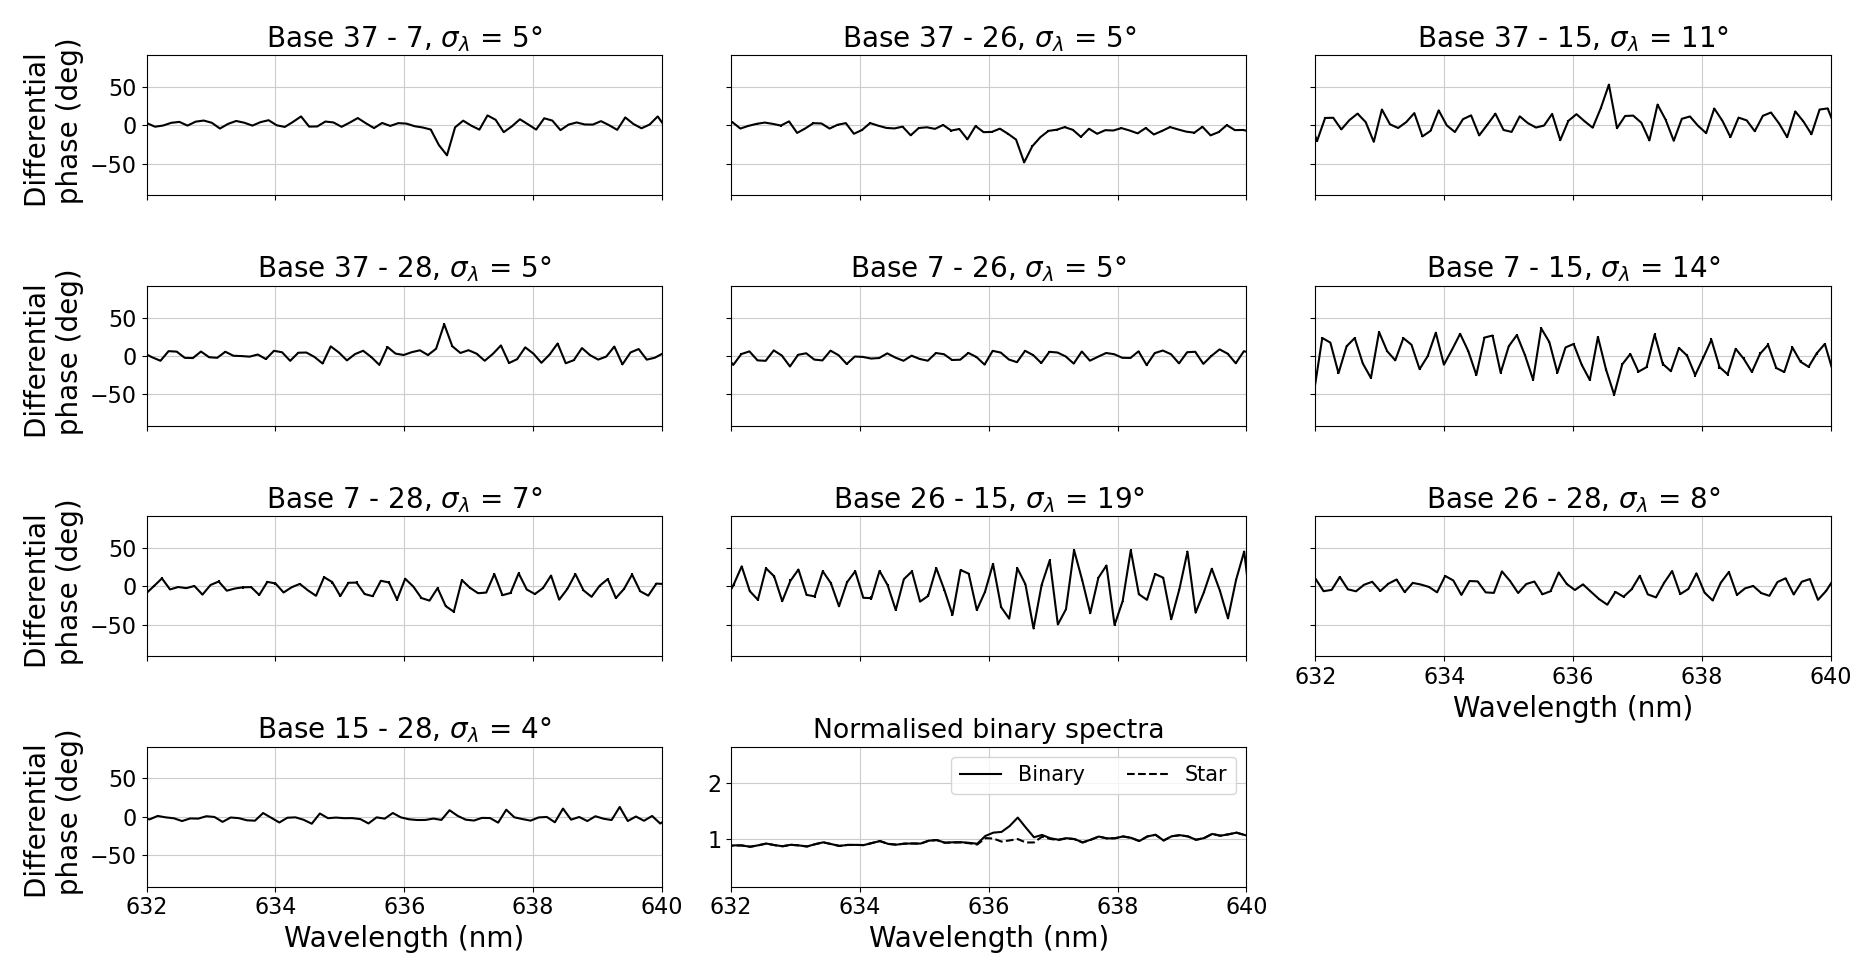
\includegraphics[width=\textwidth]{Figure_Chap4/20221010_Bin01_SpeDiffPhase_Calp2vm_BaseSubplot_Pola1_LaTex.png}
    \end{subfigure}
    \caption[Phases différentielles de la source protoplanétaire mesurée par FIRSTv2.]{Phases différentielles de la source protoplanétaire mesurée par FIRSTv2, sur toutes les bases, en fonction de la longueur d'onde. Le graphique du haut présente les phases avant et le graphique du bas présente les phases après l'étalonnage par les phases différentielles de la source non résolue. On note que l'étalonnage n'a pas réduit l'amplitude des \wiggles~mais seulement la pente globale.}
    \label{fig:PhaseDiffBinary}
\end{figure}

Le graphique du bas de la figure~\ref{fig:PhaseDiffBinary} montre l'étalonnage par la soustraction des phases différentielles mesurées sur l'étoile seule. Les perturbations de basses fréquences (ici vues comme une pente à cause du zoom sur la bande spectrale) sont corrigées et le signal de phase est centré sur zéro. L'écart-type moyen des \wiggles~est égal à $8 \pm 1\degree$ sur toutes les bases et par comparaison entre les deux graphiques, il a parfois augmenté (pour les bases $37-26$, $7-11$, $37-28$, $26-28$ et $15-28$). Les \wiggles~n'ont donc pas été corrigés par cet étalonnage. Une telle erreur sur la phase par les \wiggles~correspond à un contraste de $0,14$, ce qui est insuffisant par rapport aux performances nécessaires pour étudier le cas scientifique des protoplanètes.

Dans le cadre d'observations sur les cibles du cas scientifique auquel cette thèse s'intéresse (e.g. la protoplanète PDS 70 b, voir la section~\ref{sec:pds70}), l'objectif est de mesurer des signaux de phase d'amplitude $\sim 1\degree$ (correspondant à un contraste de $\sim 2.10^{-2}$) ce qui est bien plus faible que les \wiggles~observés ici. Ces perturbations limitent les capacités de l'instrument et il est alors crucial d'identifier leur cause afin de réussir à les réduire. Une étude de ceux-ci est présentée plus tard dans la section~\ref{sec:wiggles}.


%%%%%%%%%%%%%%%%
\subsection{Résultats de l'ajustement du modèle de protoplanète sur les phases différentielles}

Nous continuons cependant à étalonner les phases différentielles car cela corrige les pentes globales comme nous l'avons vu dans la partie précédente. Il s'agit maintenant de les ajuster au modèle de la protoplanète. Pour ce faire, je calcule les paramètres ($\rho, \alpha, \beta$) qui minimisent la fonction de l'équation~\ref{eq:chi2}, dans le canal spectral du pic central de la raie d'émission du compagnon ($635 \,$nm). Les intervalles de ces paramètres sur lesquels le calcul de la fonction $\chi^2$ est effectué, sont définis comme suit :

\begin{itemize}
    \item le contraste entre l'étoile et le compagnon sur le canal spectral où se situe le pic d'émission, $\rho \in [0,05; 0,995]$ avec un pas de $0,005$, constituant $190$ valeurs;
    \item la coordonnée du compagnon $\alpha \in [-100; 100]\,$as avec un pas de $0,5 \,$as, constituant $400$ valeurs;
    \item la coordonnée du compagnon $\beta \in [-100; 100]\,$as avec un pas de $0,5 \,$as, constituant $400$ valeurs.
\end{itemize}

La minimisation de la fonction $\chi^2$ est donc faite dans un espace de paramètres de dimension $190 \times 400 \times 400$. De plus, j'exclus les phases différentielles des bases $7-15$ et $26-15$ au cours de cette minimisation car ce sont les deux bases pour lesquelles les \wiggles~sont très intenses. La minimisation est donc effectuée sur huit des dix bases. La figure~\ref{fig:PhaseDiffBin01LikeliMap} présente la carte des valeurs maxima de la fonction de vraisemblance $\Like$ selon la dimension du contraste, en fonction des coordonnées ($\alpha, \beta$). Le cercle noir a pour rayon la séparation théorique du système protoplanétaire ($\sim 87,3\,$as), la croix noire indique la position de la source centrale et la croix rouge indique la position trouvée après marginalisation de la fonction de vraisemblance sur les deux paramètres de positions $(\alpha; \beta)$, estimés ici à $-87\substack{+4 \\ -3} \,$as et $0\substack{+1 \\ -1} \,$as, respectivement. Le contraste de la source est estimé à $0,68\substack{+0,05 \\ -0,04}$. On remarque que deux maxima locaux principaux sont trouvés sur la carte, ce qui est cohérent avec les graphiques de la figure~\ref{fig:PhaseDiffBinSizeSimule}, sur lesquelles on peut identifier une dégénérescence du signal avec une période de $\uplambda / \text{B}_{\text{min}} = 124,7 \,$as. Ainsi, le deuxième maximum est (théoriquement) localisé à $-87,3 + 124,7 = 37,4 \,$as. Pour discriminer la séparation du compagnon sur la carte de la vraisemblance, il est nécessaire d'effectuer une mesure avec une base d'une troisième longueur, pour sonder une troisième fréquence spatiale. Étant donné que nous connaissons la séparation angulaire du système observé (indiquée par le cercle noir sur la carte), je ne considère que le minimum local qui en est le plus proche, lors de l'estimation des trois paramètres.

\begin{figure}[ht!]
    \centering
    \begin{subfigure}{0.5\textwidth}
        \centering
        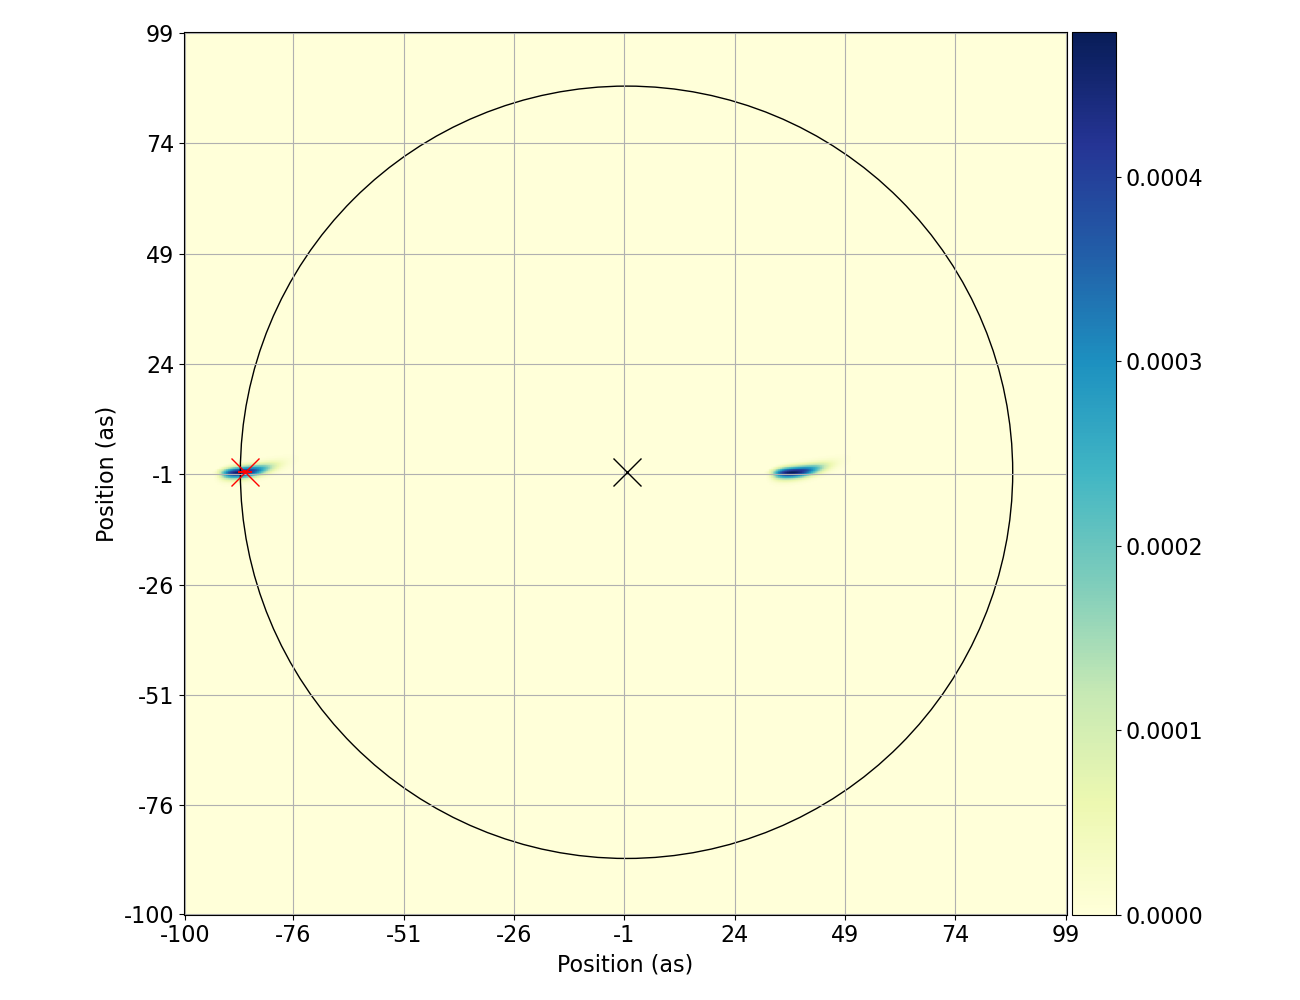
\includegraphics[width=\textwidth]{Figure_Chap4/20221010_Bin01_SpeDiffPhase_FitLikeli_Map_Pola1_LaTex.png}
    \end{subfigure}%
    \begin{subfigure}{0.5\textwidth}
        \centering
        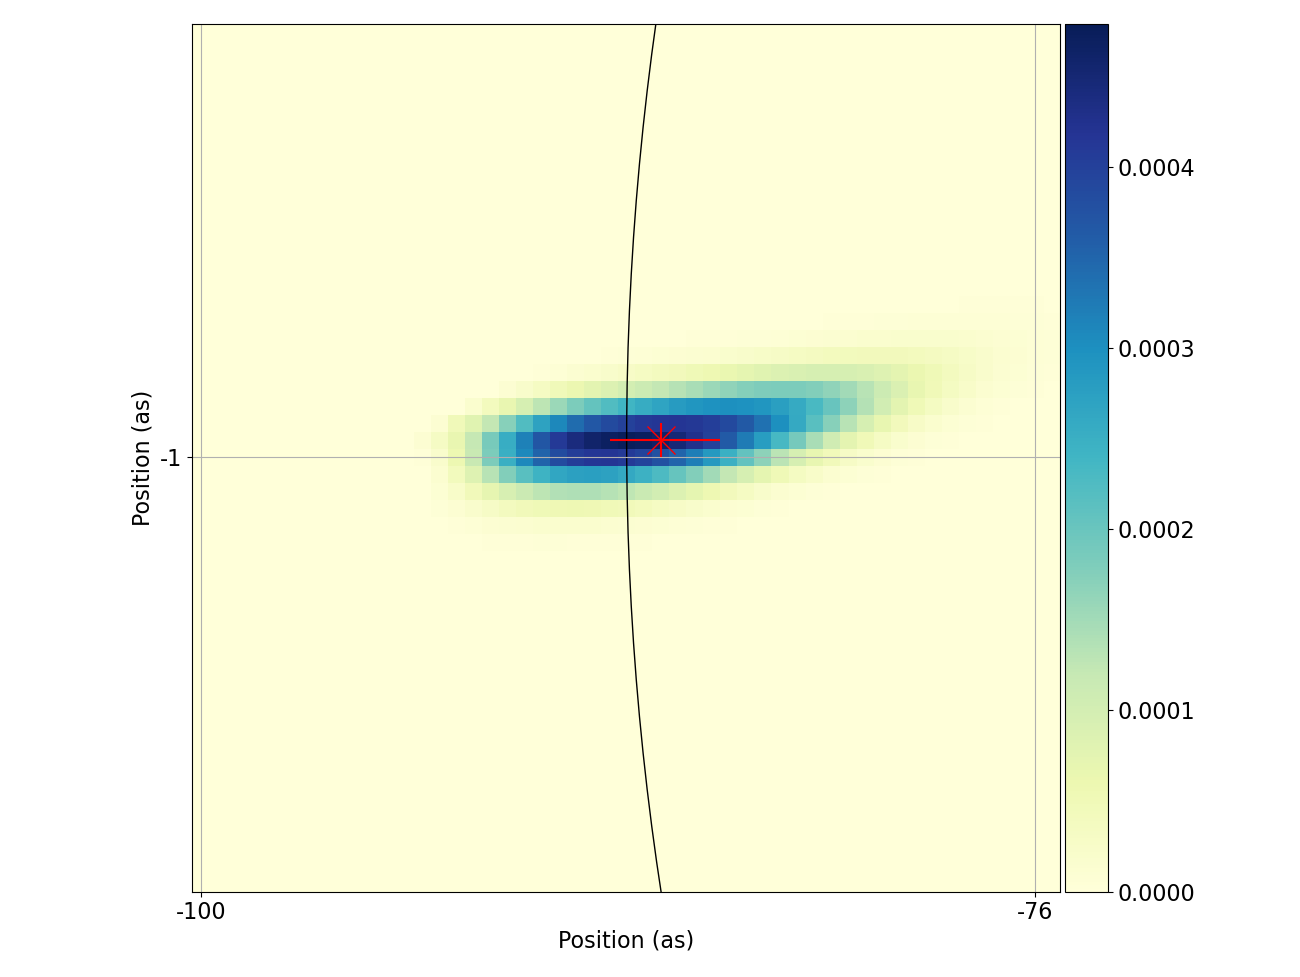
\includegraphics[width=\textwidth]{Figure_Chap4/20221010_Bin01_SpeDiffPhase_FitLikeli_MapZoom_Pola1_LaTex.png}
    \end{subfigure}
    \caption[Carte de la fonction de vraisemblance calculée à partir des phases différentielles mesurées sur la puce $Y$.]{Carte de la fonction de vraisemblance (à gauche) calculée à partir des phases différentielles mesurées sur la puce $Y$, en fonction des coordonnées ($\alpha; \beta$) et zoom centré sur la croix rouge (à droite). La croix noire indique la position de la source centrale ($0; 0$) et la croix rouge indique la position la plus probable à partir de la marginalisation de la vraisemblance ($-87\substack{+4 \\ -3}; 0\substack{+1 \\ -1} \,$)as, trouvé pour un contraste de $0,68\substack{+0,05 \\ -0,04}$. Le cercle noir a pour centre la croix noire et pour rayon la séparation angulaire attendue du compagnon.}
    \label{fig:PhaseDiffBin01LikeliMap}
\end{figure}

À partir des paramètres optimaux trouvés précédemment, je trace les phases différentielles en utilisant l'équation~\ref{eq:PhaseBinaireCentree} sur la figure~\ref{fig:PhaseDiffBin01LikeliFit}, en pointillés, superposées aux phases différentielles mesurées, en trait plein. Les phases différentielles estimées des bases $7-15$ et $26-15$ exclues de la minimisation, sont laissées à zéro. La comparaison des deux montre qu'on a bien réussi à estimer les trois paramètres qui ajustent les courbes de phases mesurées.

\begin{figure}[ht!]
    \centering
    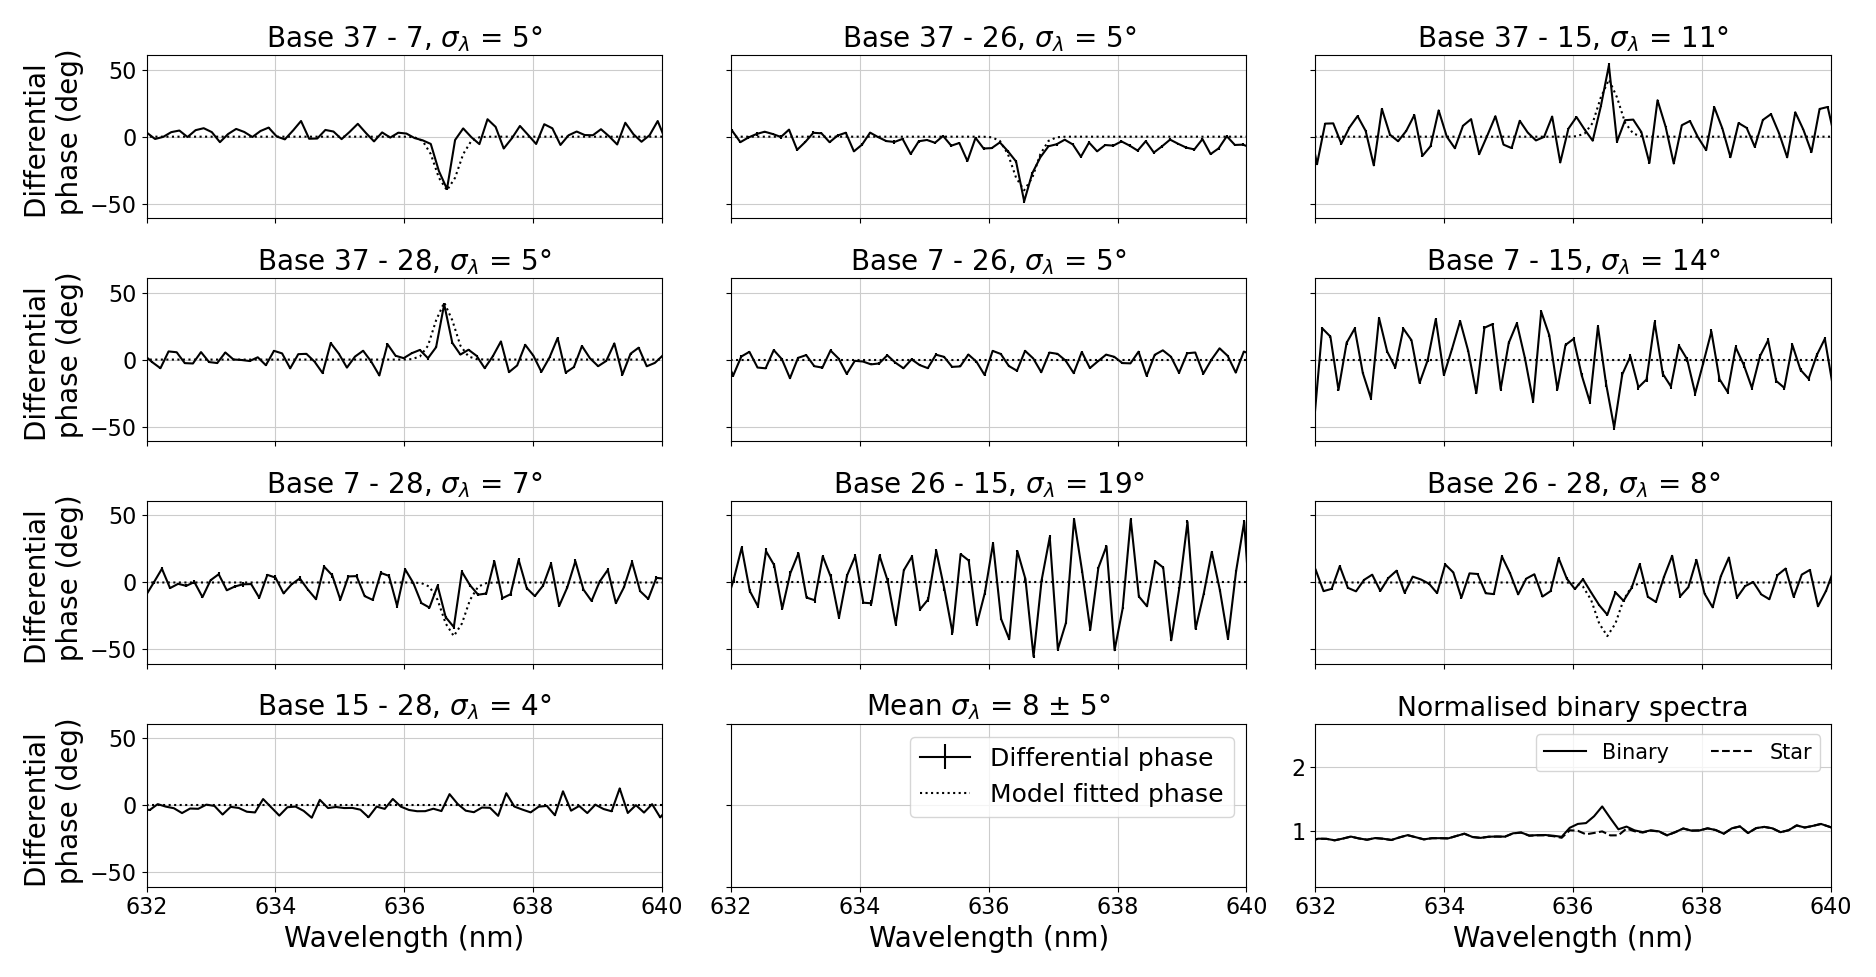
\includegraphics[width=\figwidth]{Figure_Chap4/20221010_Bin01_SpeDiffPhase_Calp2vm_FitLikeli_BaseSubplot_Pola1_LaTex.png}
    \caption[Graphique des phases différentielles mesurées et des phases différentielles modélisées à partir des paramètres d'ajustement du modèle de système protoplanétaire.]{Graphique des phases différentielles mesurées (en trait plein) et des phases différentielles modélisées (en pointillés) à partir des paramètres d'ajustement du modèle de système protoplanétaire. Les paramètres optimaux utilisés pour le calcul des phases à partir de ce modèle sont : ($\rho; \alpha; \beta$) = ($0,68$; $-87$; $0$).}
    \label{fig:PhaseDiffBin01LikeliFit}
\end{figure}

La même étude est faite pour des données acquises sur la source protoplanétaire avec un contraste légèrement plus élevé. La figure~\ref{fig:PhaseDiffBin02LikeliFit} présente les phases différentielles mesurées superposées au modèle calculé à partir des paramètres optimaux de la marginalisation de la fonction $\Like$. Comme précédemment, la carte résultante de la vraisemblance est montrée sur la figure~\ref{fig:PhaseDiffBin02LikeliMap}. Le contraste de cette source est estimé à $0,57 \pm 0,06$ et les coordonnées de la séparation angulaire sont estimées à ($-87\substack{+16 \\ -4}; 1\substack{+2 \\ -1} \,$)as. La carte de la vraisemblance présente deux maxima locaux en plus que sur la première carte. Cela est dû au fait que le signal du pic de phase du compagnon est plus faible, ce qui diminue le \ac{SNR} des données, entraînant une difficulté accrue de l'estimation des paramètres optimaux. Par conséquent, on peut estimer que la limite inférieure du contraste d'une source protoplanétaire détectable par le banc de test actuel de \ac{FIRSTv2} est d'environ $0,55$.

\begin{figure}[ht!]
    \centering
    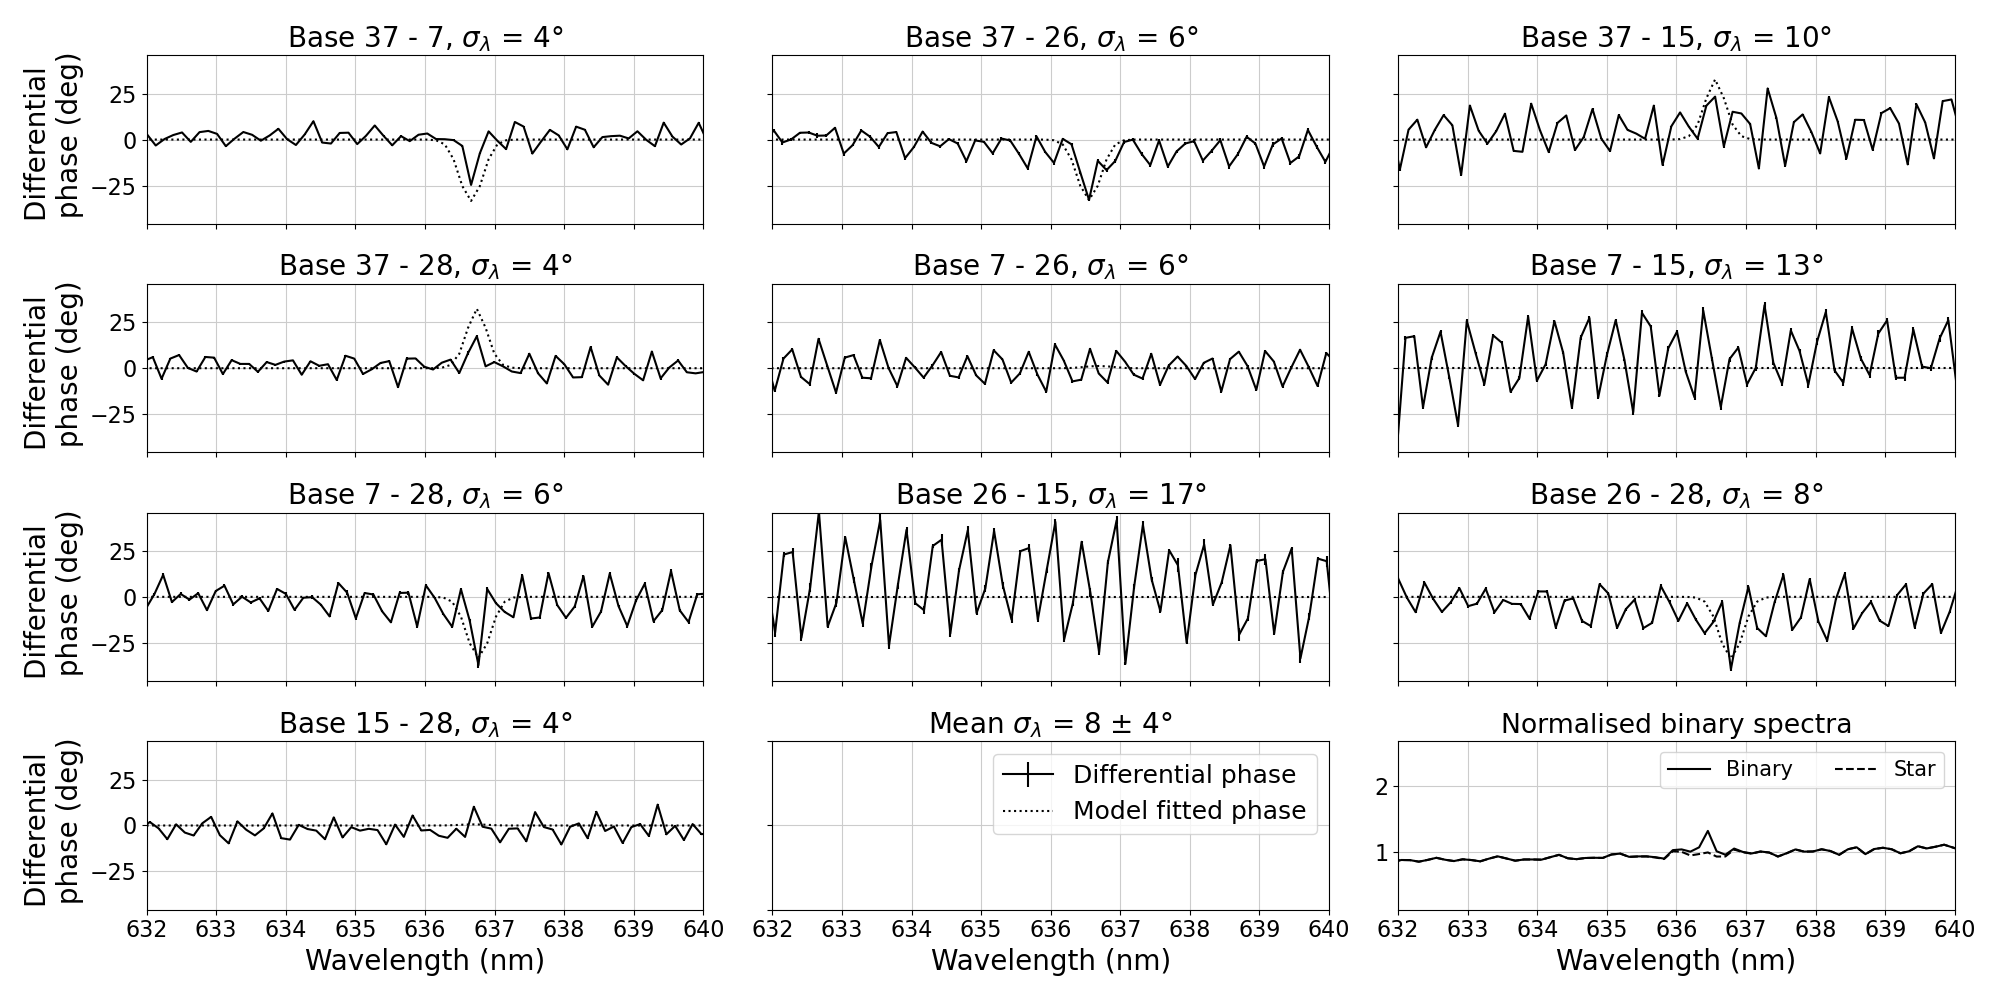
\includegraphics[width=\figwidth]{Figure_Chap4/20221010_Bin02_SpeDiffPhase_Calp2vm_FitLikeli_BaseSubplot_Pola1_LaTex.png}
    \caption[Graphique des phases différentielles mesurées et des phases différentielles modélisées à partir des paramètres d'ajustement du modèle de système protoplanétaire.]{Graphique des phases différentielles mesurées (en trait plein) et des phases différentielles modélisées (en pointillés) à partir des paramètres d'ajustement du modèle de protoplanète. Les paramètres optimaux utilisés pour le calcul des phases à partir de ce modèle sont : ($\rho; \alpha; \beta$) = ($0,57$; $-87$; $1$).}
    \label{fig:PhaseDiffBin02LikeliFit}
\end{figure}

\begin{figure}[ht!]
    \centering
    \begin{subfigure}{0.5\textwidth}
        \centering
        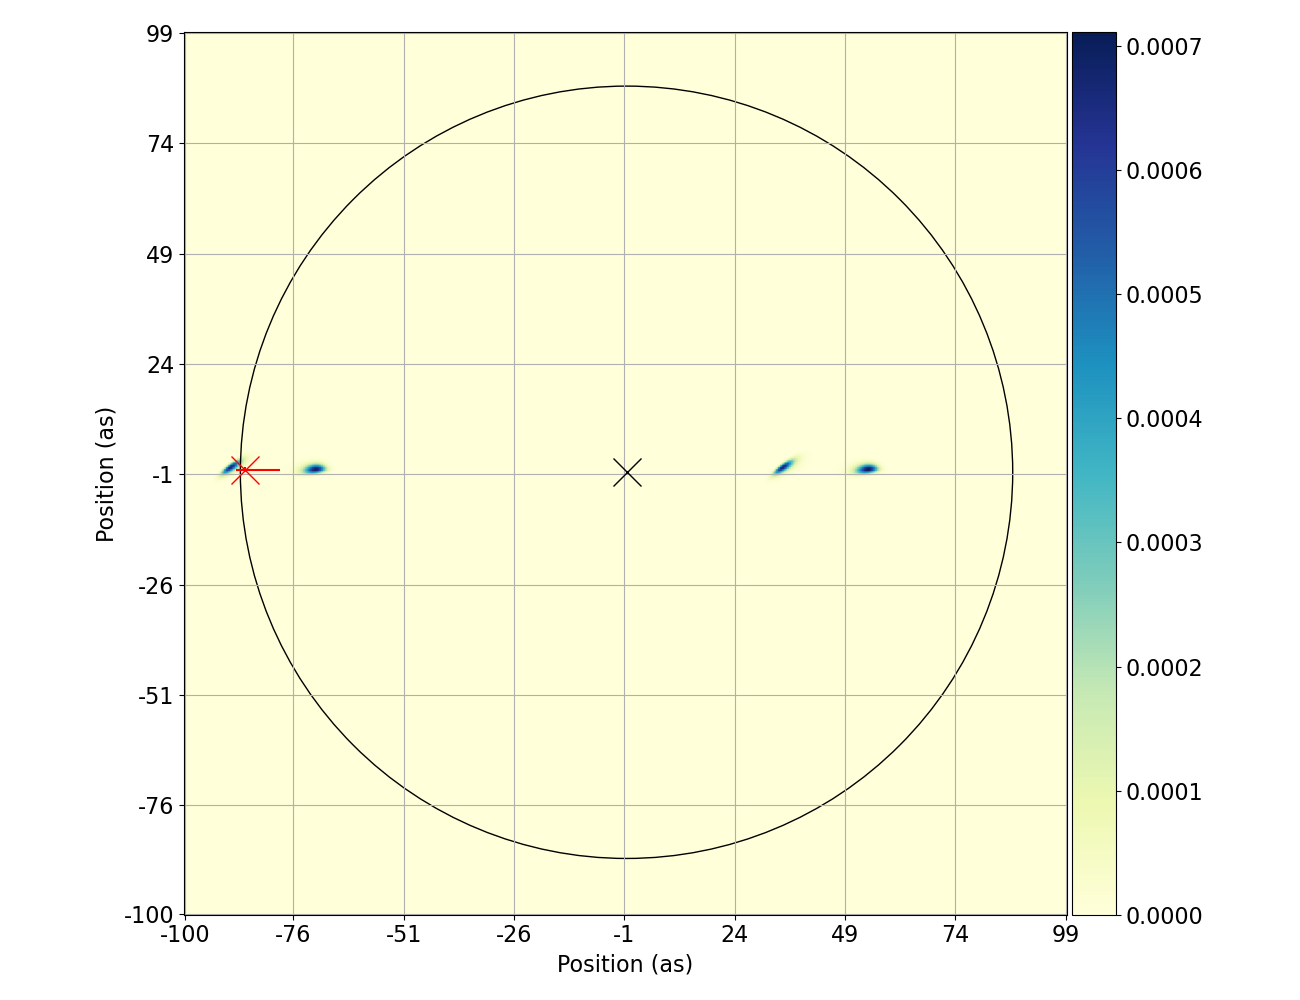
\includegraphics[width=\textwidth]{Figure_Chap4/20221010_Bin02_SpeDiffPhase_FitLikeli_Map_Pola1_LaTex.png}
    \end{subfigure}%
    \begin{subfigure}{0.5\textwidth}
        \centering
        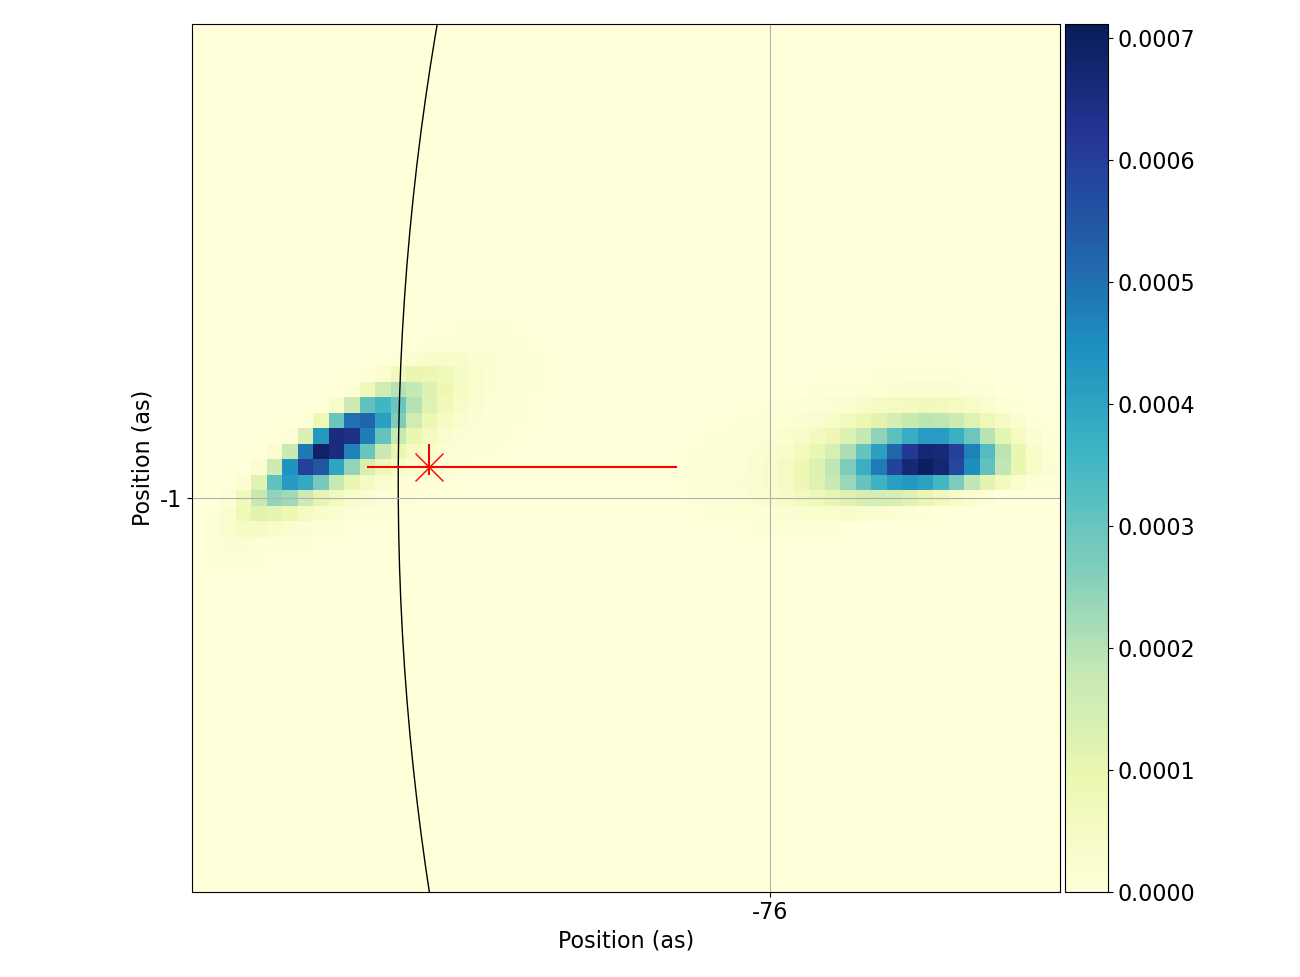
\includegraphics[width=\textwidth]{Figure_Chap4/20221010_Bin02_SpeDiffPhase_FitLikeli_MapZoom_Pola1_LaTex.png}
    \end{subfigure}
    \caption[Carte de la fonction de vraisemblance calculée à partir des phases différentielles mesurées sur la puce $Y$.]{Carte de la fonction de vraisemblance (à gauche) calculée à partir des phases différentielles mesurées sur la puce $Y$, en fonction des coordonnées ($\alpha, \beta$) et zoom centré sur la croix rouge (à droite). La croix noire indique la position de la source centrale et la croix rouge indique la position la plus probable à partir de la marginalisation de la vraisemblance ($-87\substack{+16 \\ -4}; 1\substack{+2 \\ -1} \,$)as, trouvé pour un contraste de $0,57 \pm 0,06$. Le cercle noir a pour centre la croix noire et pour rayon la séparation angulaire attendue du compagnon.}
    \label{fig:PhaseDiffBin02LikeliMap}
\end{figure}


%%%%%%%%%%%%%%%%%%%%%%%%%%%%%%%%
\section{Les wiggles}
\label{sec:wiggles}

%%%%%%%%%%%%%%%%
\subsection{Les wiggles sur d'autres instruments}

Dans cette partie je présente une étude réalisée sur les \wiggles~mesurés sur les données de \ac{FIRSTv2} afin de les caractériser. Mais tout d'abord, je fais la liste de plusieurs expériences sur lesquelles ce phénomène a déjà été mesuré :

\begin{itemize}
    \item les \wiggles~sont visibles sur les phases différentielles d'\ac{AMBER} \citep{millour2008} et leur cause a été identifiée comme provenant d'une cavité Fabry-Pérot créée par la lame d'air présente dans les polariseurs \citep{malbet2008}, ce qui a permis de totalement les corriger en optant pour des polariseurs à lame mince;
    \item les \wiggles~sont aussi visibles sur les phases différentielles de \ac{GRAVITY} \citep{amorim2020} mais sont d'assez faible amplitude pour ne pas gêner les mesures. A la suite de discussions privées avec Nicolas Pourré, doctorant sur le projet \ac{GRAVITY}, il semblerait que le même phénomène soit mesuré et visible sur la norme et la phase des visibilités complexes;
    \item des franges spectrales sont aussi visibles sur les données de l'instrument \ac{MIRI} du \ac{JWST} \citep{argyriou2020} et leur cause est identifiée comme provenant d'une cavité Fabry-Pérot créée par les différentes couches électroniques de la caméra. Les \wiggles~sont corrigés au cours du traitement de données, par ajustement de la fonction de transmission Fabry-Pérot.
\end{itemize}


%%%%%%%%%%%%%%%%
\subsection{Première analyse des wiggles sur FIRSTv2}

Les \wiggles~sur le banc de test de \ac{FIRSTv2} apparaissent sur toutes les images. La figure~\ref{fig:WigglesFlat} présente le spectre mesuré sur une des sorties imagées sur la caméra, lorsque une seule entrée est illuminée. Il s'agit donc d'un spectre sans frange d'interférence, sur toute la bande spectrale transmise (en haut) et sur une bande comprise entre $660 \,$nm et $690 \,$nm (en bas). On note que les \wiggles~apparaissent sur toute la bande spectrale et leur période est estimée à $\sim 0,5 \,$nm. Une rapide analyse montre que cette période est constante en fonction du nombre d'onde $\sigma$.

\begin{figure}[ht!]
    \centering
    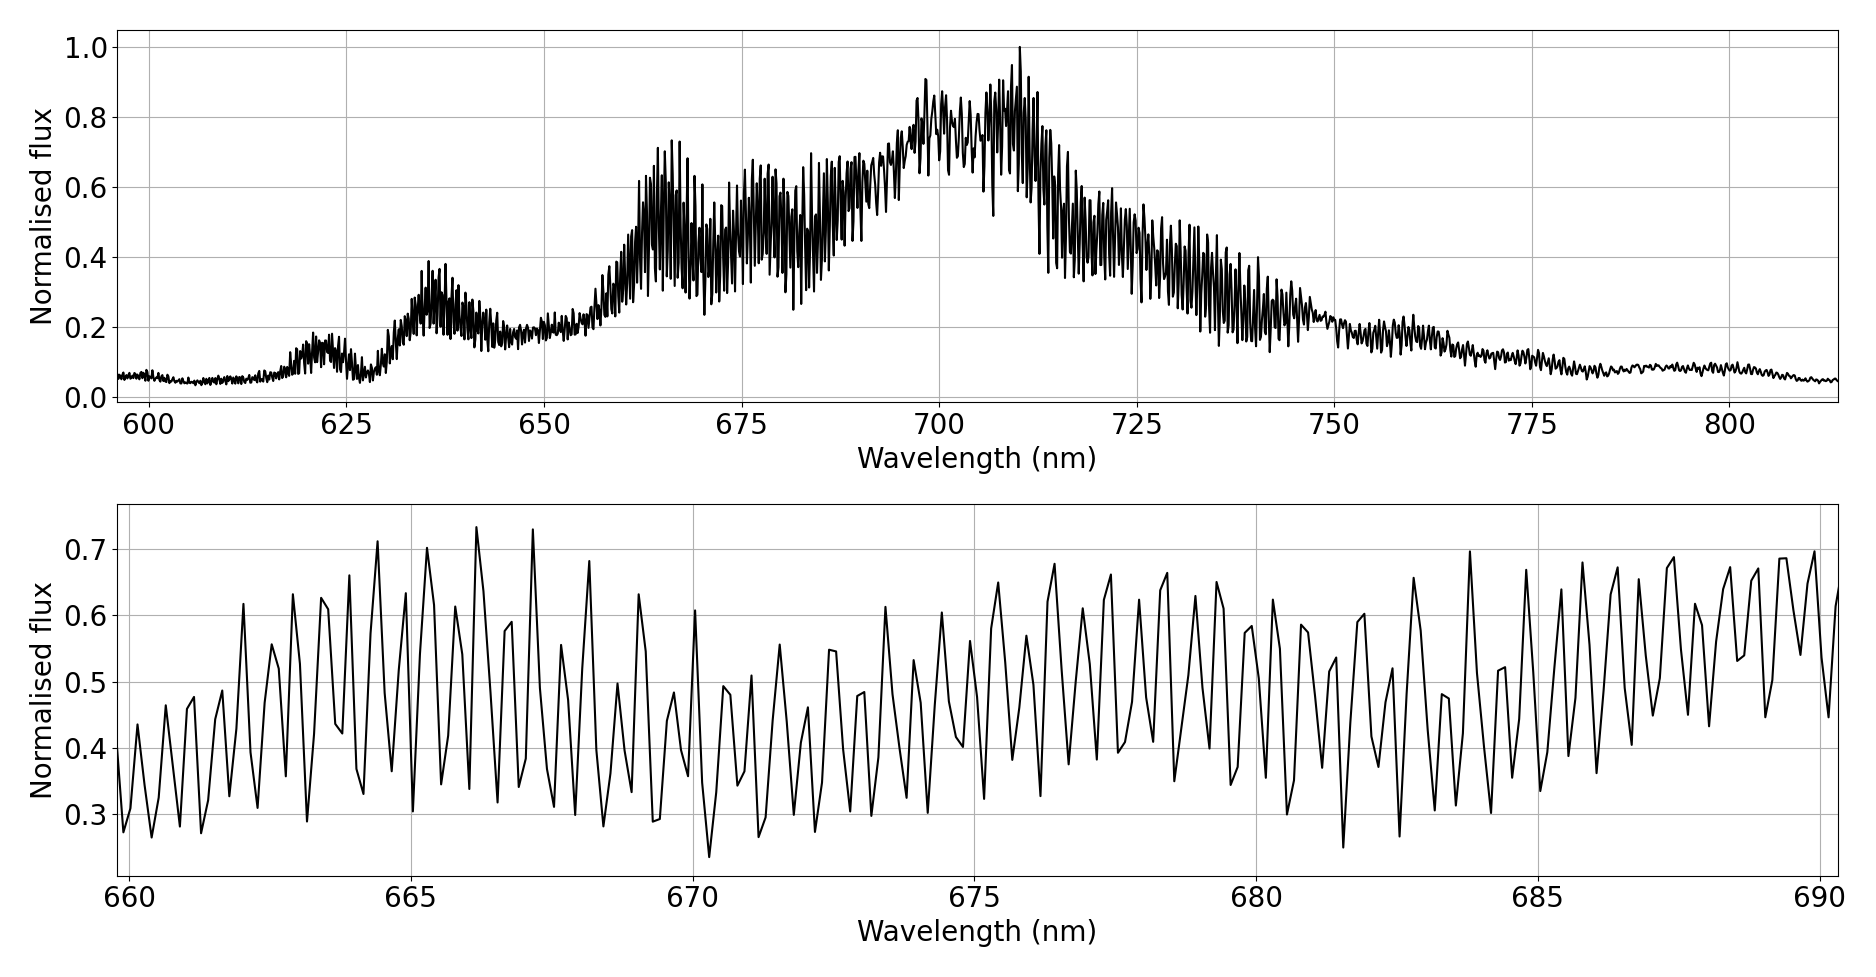
\includegraphics[width=\figwidth]{Figure_Chap4/20220811_P2VM_01_Flat1_1_FluxVSWave_Pola1.png}
    \caption[Spectre présentant des wiggles mesuré sur une sortie sans frange d'interférence, sur FIRSTv2.]{Spectre normalisé présentant des wiggles mesuré sur une sortie sans frange d'interférence, sur FIRSTv2. Le spectre est tracé sur toute la bande spectrale transmise par FIRSTv2 (en haut) et sur la bande comprise entre $660 \,$nm et $690 \,$nm (en bas).}
    \label{fig:WigglesFlat}
\end{figure}

Un filtrage fréquentiel pourrait être utilisé afin de corriger ces perturbations. Lors d'un traitement préliminaire dans lequel un filtrage passe-bas a été appliqué aux mesures de phases différentielles sur le système protoplanétaire simulé, il a été remarqué que le filtrage pouvait détériorer la raie du compagnon (diminuant son amplitude jusqu'à un facteur $2$). Cela parait cohérent puisque la largeur de la raie du compagnon est du même ordre de grandeur que la largeur des \wiggles. Ainsi, il a été choisi pour l'instant de ne pas appliquer de filtrage spatial sur les phases différentielles.

% Tests done at the lab to understand the cause
% Harry-Dean study:
% - tests on different polarizers with differents thickness => didn't change the wiggles frequency
% - no polar + Wolla in spectro => no wiggles
% - 2 wolla => wiggles
% - data without the chip and without polar/Wolla => no wiggles
% ==> il semble que cela vienne des fibres et du fait qu'on sélectionne la polar injectée
De récentes mesures effectuées sur le banc par Manon Lallement et Harry-Dean Kenchington Goldsmith semblent montrer que les puces ne sont pas la seule cause des \wiggles. Plusieurs tests ont été faits en injectant la source \sk~dans le montage suivant : (1) polariseur, (2) fibre optique, (3) monture pour fibre optique avec la rotation autour de l'axe $Z$ comme degré de liberté, (4) le spectro-imageur et (5) la caméra. Différents tests mènent aux observations suivantes :

\begin{itemize}
    \item en utilisant des polariseurs de différentes épaisseurs (avant ou après la fibre), la période des \wiggles~reste inchangée, ce qui montre qu'ils ne sont pas causés par une cavité Fabry-Pérot créée par le polariseur;
    \item en retirant le polariseur en entrée de fibre, les \wiggles~disparaissent;
    \item en utilisant un prisme de wollaston en entrée de fibre, les \wiggles~sont visibles;
    \item les \wiggles~disparaissent pour certaines valeurs d'angle de la fibre optique en entrée du spectro-imageur.
\end{itemize}

On peut déduire de ces observations qu'il semblerait que la sélection d'une polarisation avant l'injection des faisceaux dans les fibres soit la cause de l'apparition des \wiggles. En effet, la biréfringence des fibres optiques impose l'injection de lumière polarisée dans le sens de son axe. Autrement, la polarisation est elliptique en sortie de la fibre et interfère avec elle-même. Il semble donc nécessaire de s'assurer que l'axe de polarisation de tous les composants utilisés sur le banc de test (polariseur, fibres optiques, puce photonique, prisme de Wollaston) soient alignés. Les extrémités des fibres optiques sont montées sur les férules de sorte que leurs axes principaux de polarisation soient alignés quand on les raccorde. Cela signifie qu'il serait nécessaire de les aligner avec plus de précision à l'avenir.

De plus amples investigations sont nécessaires et sont toujours conduites afin de comprendre totalement l'origine de ces perturbations et de déterminer une solution pour contourner ce problème.


%%%%%%%%%%%%%%%%%%%%%%%%%%%%%%%%
\section{Conclusion}
% en parlant de bruit, je me demande si on ne pourrait pas te demander à quelle magnitude équivalente le signal avec lequel tu travailles correspond. Mais ce n'est pas simple comme question... Sylvestre tu as peut être une idée sur ce point ?

Dans ce chapitre j'ai présenté le simulateur de source protoplanétaire que j'ai mis en place sur le banc de test, ce qui a été primordial pour le développement de \ac{FIRSTv2} pour la caractérisation de systèmes protoplanétaires. Les mesures que j'ai présentées montrent la validité de la technique des phases différentielles mesurées sur une source de type protoplanétaire, présentant un contraste plus faible sur une bande spectrale étroite.

J'ai ainsi montré la détection d'un compagnon à une séparation de $0,68 \lambda / B$ avec un contraste égal à $\sim 0,55$, à partir du calcul et de l'analyse des phases différentielles. Le contraste atteint dans cette étude est encore assez faible comparé au contraste des protoplanètes que l'on connaît actuellement (contraste de $\sim 10^{-2} - 10^{-3}$ pour la protoplanète PDS 70 b). En effet, les mesures de phases différentielles sont limitées par les \wiggles~dont l'erreur moyenne qu'elle ajoute est estimée à $\sim 8\degree$, correspondant à un contraste de $\sim 0,14$, soit $\sim 0,56$ pour un signal de phase au moins quatre fois plus grand que les \wiggles~(\ac{SNR} $= 4$).

Une partie des efforts de l'équipe se concentre actuellement sur la compréhension de l'origine de ces \wiggles~ainsi que sur leur correction.


%%%%%%%%%%%%%%%%%%%%%%%%%%%%%%%%
\clearpage
\section*{Conférence Hypatia Colloquium}
\label{sec:HypatiaProceeding}
\phantomsection
\addcontentsline{toc}{section}{Conférence Hypatia Colloquium}

\clearpage
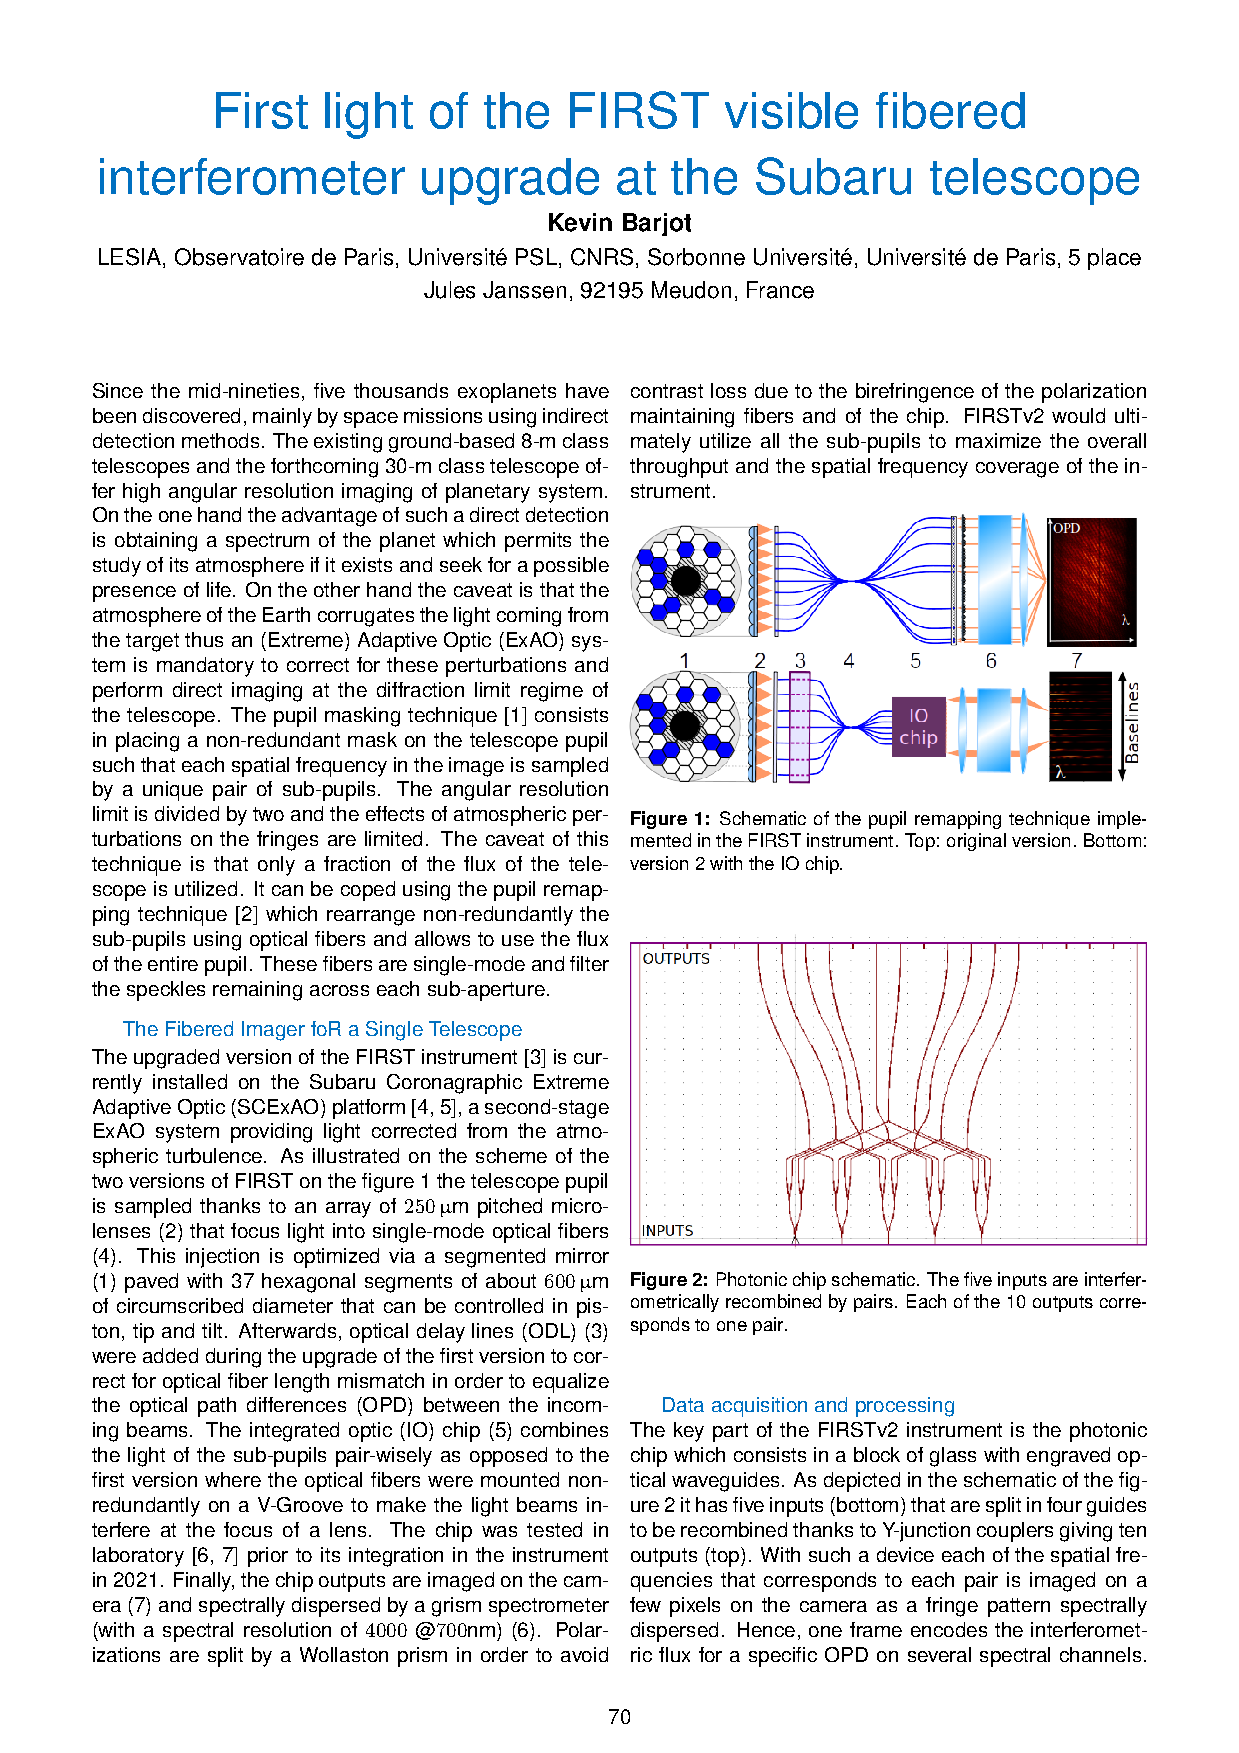
\includepdf[pages=-, pagecommand={}, offset=-10 -20, templatesize={0.8\textwidth}{0.8\textheight}]{Paper/Barjot2022_HypatiaProceeding_Pub.pdf}

% Original comprehensive wiggles part (first draft)
\begin{comment}
%%%%%%%%%%%%%%%%
\subsection{Les wiggles sur d'autres instruments}

%%%%%%%%
\subsubsection{AMBER - VLTi}

L'instrument \acrfull{AMBER} \citep{petrov2007} est un interféromètre semblable à \ac{FIRSTv1} utilisant la technique de réarrangement de pupilles avec des fibres optiques mono-modes. Trois des télescopes du \ac{VLT} interfère par une recombinaison multi-axiale et l'interférogramme obtenu est dispersé par un spectrographe à fente en bande \textit{J}, \textit{H} et \textit{K}, pouvant atteindre une résolution spectrale de \numprint{10000}. Enfin, une polarisation est sélectionnée avec un polariseur composé de deux prismes.

Afin d'étalonner les phases mesurées des perturbations instrumentales \citep{millour2008}, un système de commutation de faisceaux (\acrfull{BCD}) est utilisé et consiste à commuter deux faisceaux d'une bases pour mesurer successivement la phase et son opposé. La moitié de la soustraction des deux mesures permet alors de corriger les perturbations instrumentales en aval du \ac{BCD} (celui-ci doit donc être installé le plus en amont possible sur l'instrument). L'avantage de cette technique c'est qu'elle s'exécute sur une durée de $5 \,$s environ, ce qui est bien moindre que la boucle d'étalonnage du \ac{VLT} qui dure $30 \,$min environ, en mesurant la phase sur une étoile non résolue à proximité de la source étudiée. 

La figure~\ref{fig:AMBERMillourDiffPhase} montre les deux techniques d'étalonnage que je viens de citer : avec une étoile de référence (colonne de gauche nommée STD mode) ou avec le système \ac{BCD} (colonne de droite nommée SPA mode). Sur la première ligne de graphiques sont montrés la mesure de visibilité sur la cible d'étude en rouge et la mesure de visibilité issue de la méthode de calibration. La deuxième ligne présente les phases différentielles de ces mesures et on remarque un effet de dispersion chromatique qui se traduit par une courbure globale qui peut être ajustée par une fonction polynomiale du second degré mais aussi par une modulation de la phase qui ressemble aux \wiggles~des données de \ac{FIRSTv2}. Dans l'article, cette dernière est nommée \textit{wavelength beating} ou \textit{socks} qu'on peut traduire par une modulation chromatique de la phase. L'amplitude de cette modulation est mesurée à $17\degree$ avec une période de $\sim 0,02 \,$\um. La troisième ligne présente l'étalonnage des phases différentielles, à gauche, en soustrayant d'abord la dispersion chromatique ajustée aux mesures puis en soustrayant la phase différentielle de la cible par la phase différentielle de la référence; à droite, en calculant seulement la moitié de la soustraction de la phases du faisceau non commuté avec la phase du faisceau commuté. On note alors que les \wiggles~sont réduits dans les deux cas et sont de plus grande amplitude et moins périodiques dans le cas de l'étalonnage STD : ils sont donc plus faciles à corriger à l'issu de l'autre méthode d'étalonnage.

Ce qu'on apprend de cette étude est que les \wiggles~sont des perturbations quasi-statiques de l'instrument et qu'ils sont mieux corrigés en effectuant une mesure d'étalonnage en moins d'une minute.

\begin{figure}[ht!]
    \centering
    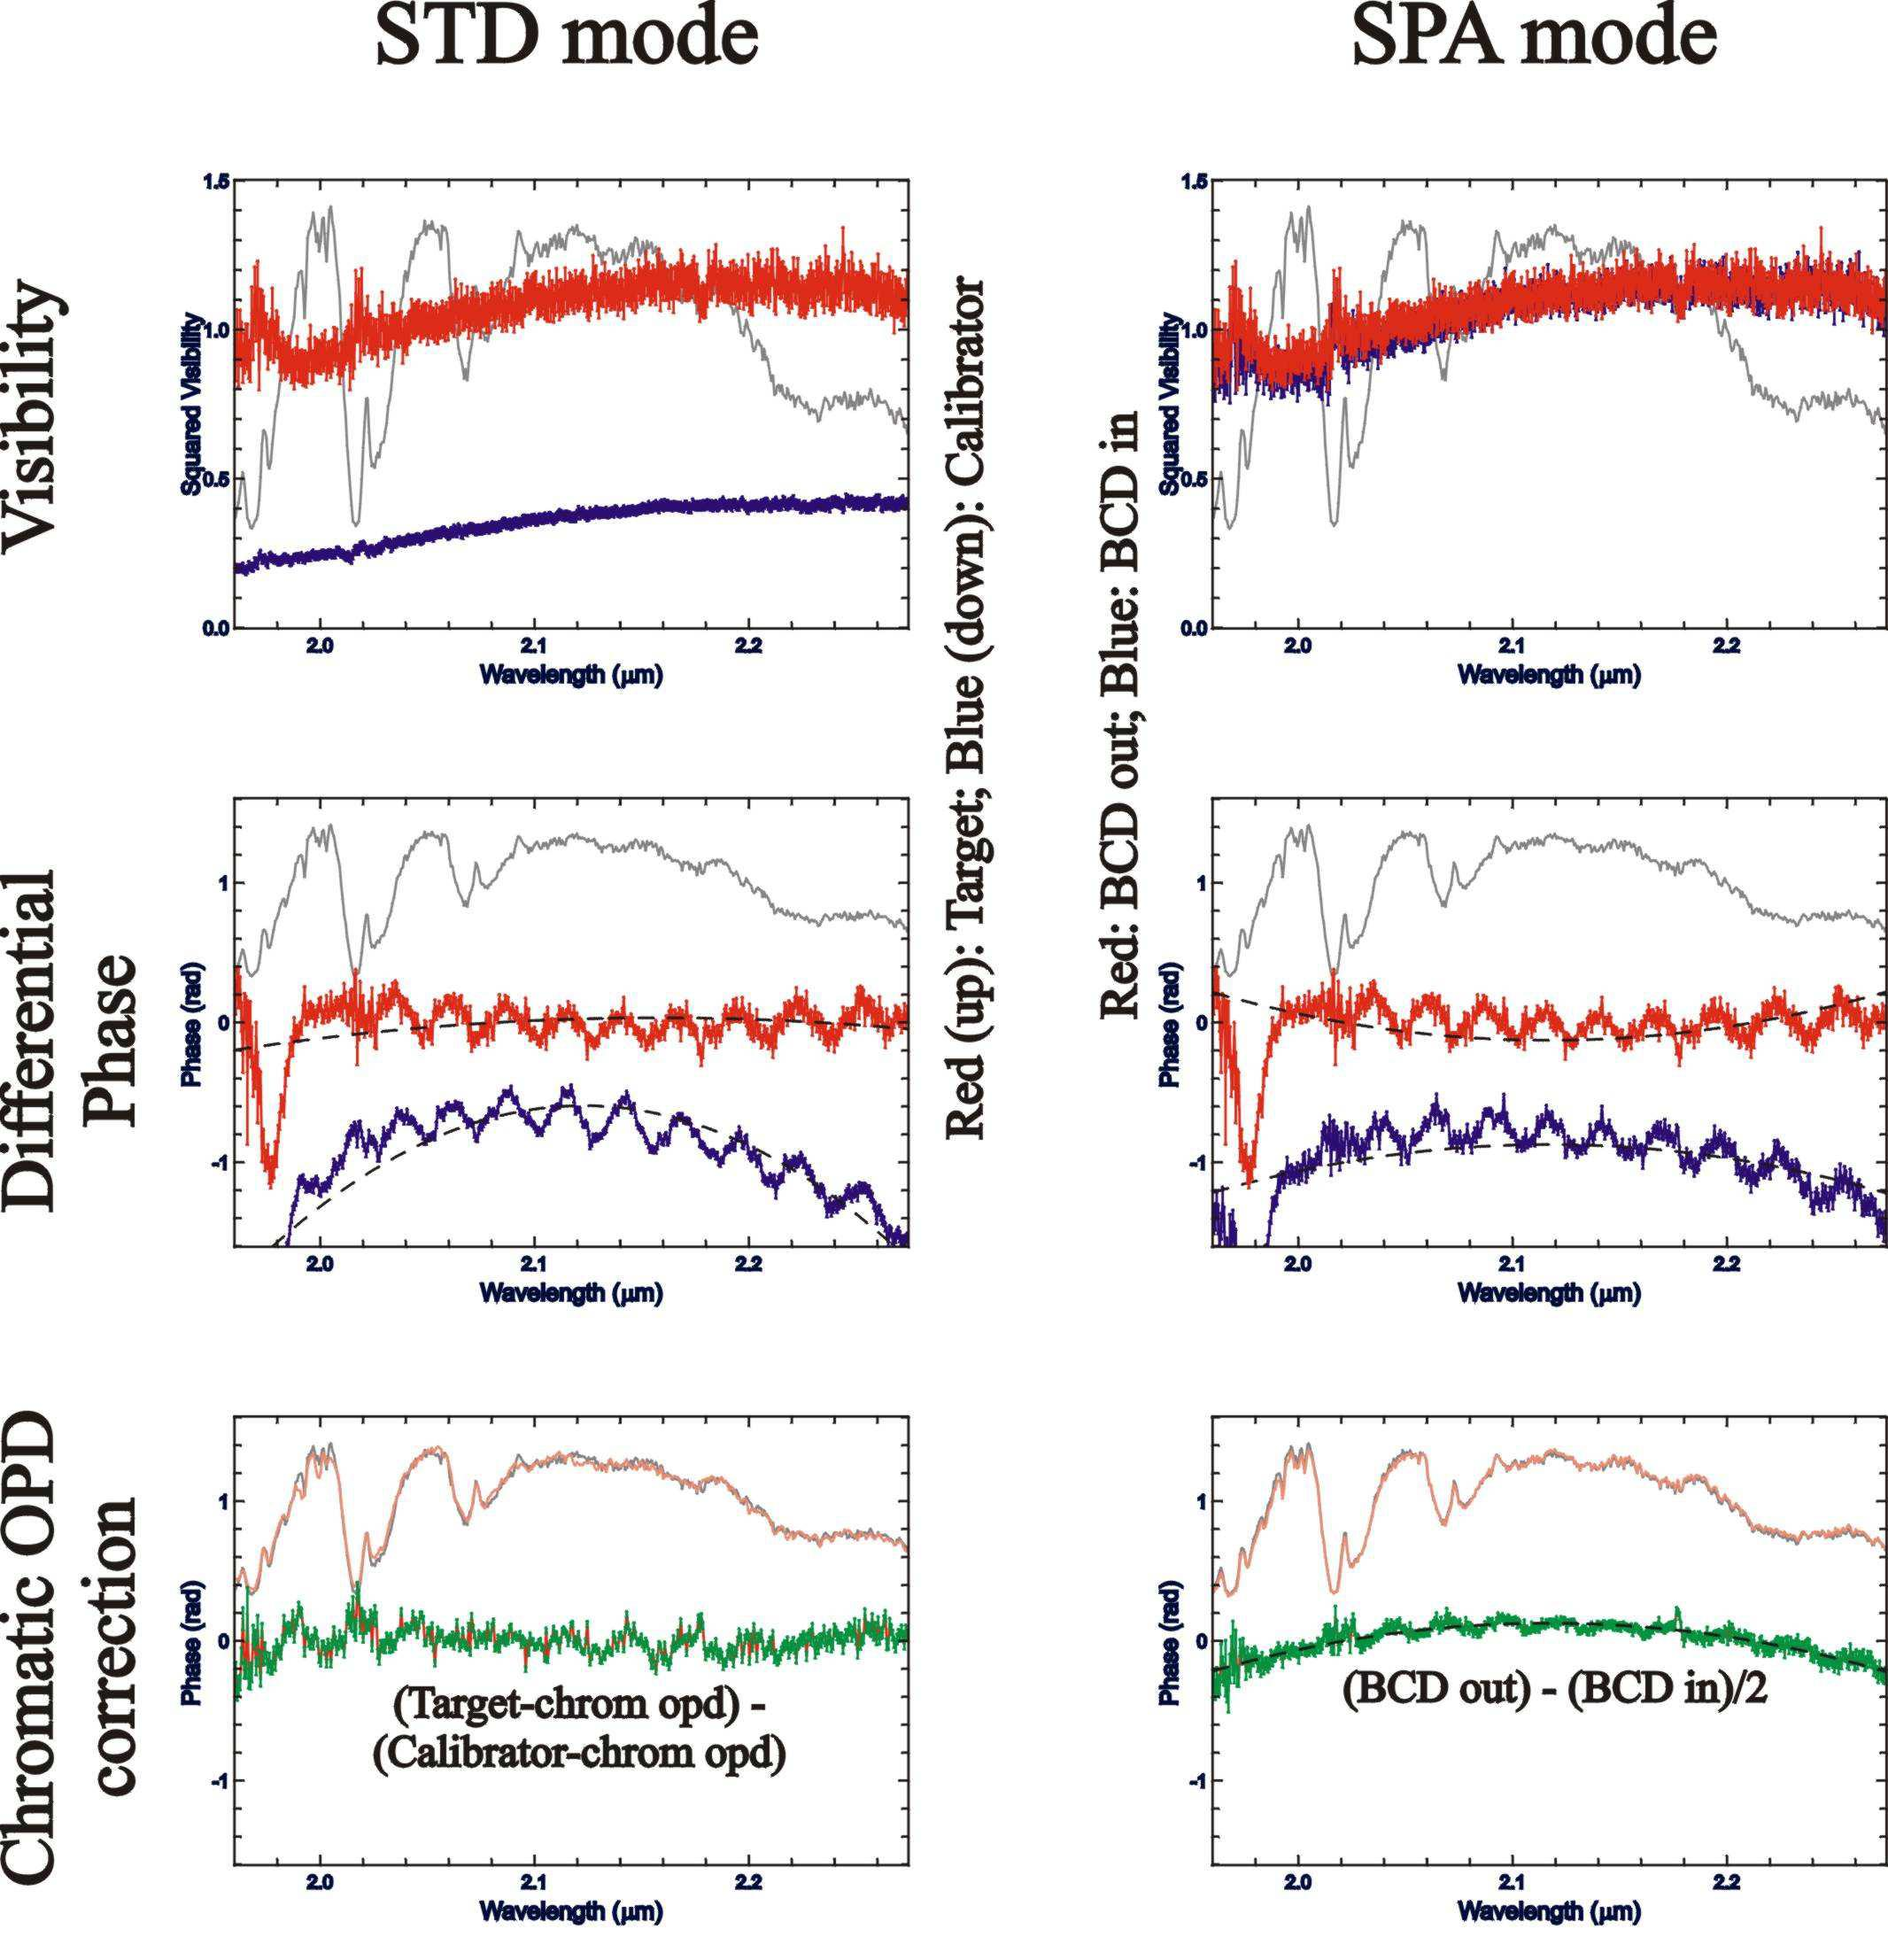
\includegraphics[width=\figwidth]{Figure_Chap4/Millour2008_Figure03_crop.png}
    \caption[]{Caption}
    \label{fig:AMBERMillourDiffPhase}
\end{figure}

Enfin, la cause de cette modulation de la phase a été identifiée comme provenant d'une cavité de Fabry-Pérot provoquée par la lame d'air présente entre les deux prismes qui composent les polariseurs. Des mesures de phases avec et sans ces polariseurs montrent que dans le deuxième cas la modulation disparaît complètement \citep{malbet2008}.

\begin{figure}[ht!]
    \centering
    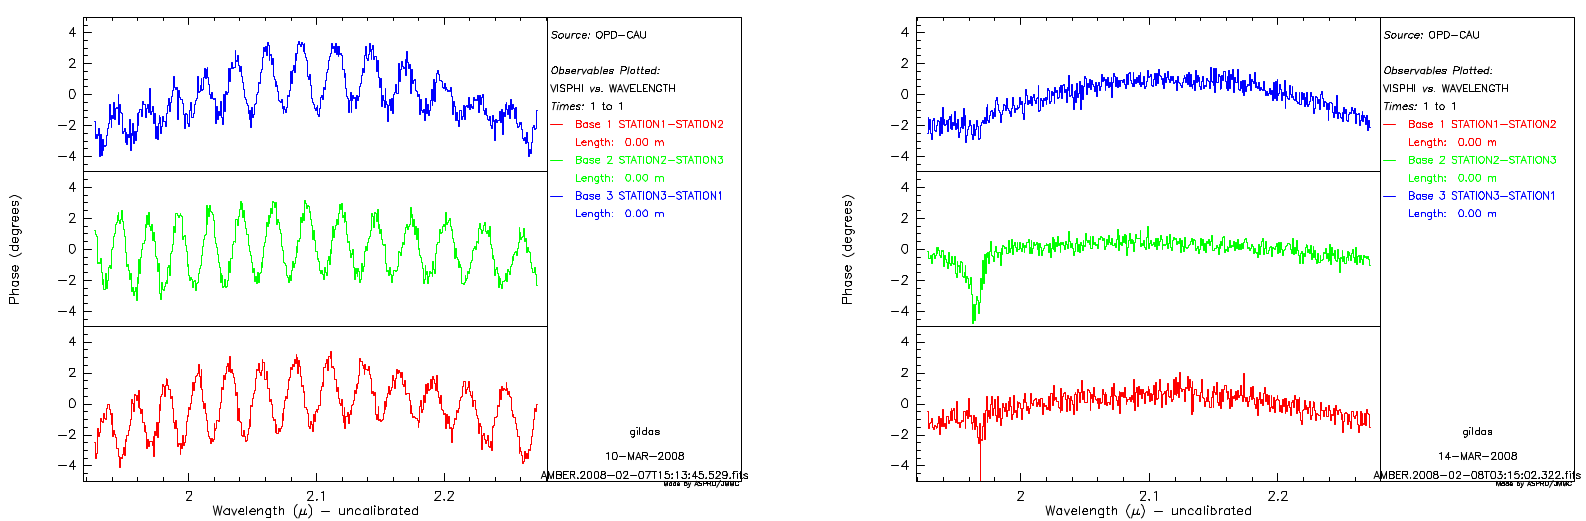
\includegraphics[width=\figwidth]{Figure_Chap4/Chelli2008_Figure01.png}
    \caption[]{Caption}
    \label{fig:AMBERChelliDiffPhase}
\end{figure}


%%%%%%%%%%%%%%%%
\subsection{Caractérisation des wiggles sur la puce X}

Cette sous-partie présente une analyse des \wiggles~sur des données acquises sur la puce $X$. Le polariseur placé juste avant l'injection des faisceaux des sous-pupilles dans les fibres optiques sélectionne la polarisation verticale (V). De plus, le prisme de wollaston est installé devant le spectrographe donc le flux des sorties correspondant à la sélection de la polarisation V est plus élevé que celui des sorties correspondant à la polarisation horizontale (H). Dans un premier temps, j'analyserai les spectres de flux sans franges d'interférences, obtenus en illuminant une à une chacune des cinq entrées de la puce.

% Comparaison à l'oeil des wiggles entre les deux polar
La figure~\ref{fig:WigglesInput1PolaComp} présente l'intensité mesurée par la caméra sur les quatre sorties illuminées par l'entrée $1$ de la puce. Les flux normalisés par le maximum en polarisation V et en polarisation H sont tracés en bleu et orange, respectivement, pour comparaison, en fonction des pixels de la caméra. Les graphiques ne sont pas cadrés sur le même intervalle de pixels et montrent que les \wiggles~ne se superposent pas de façon consistante sur les gammes de pixels montrées.

\begin{figure}[ht!]
    \centering
    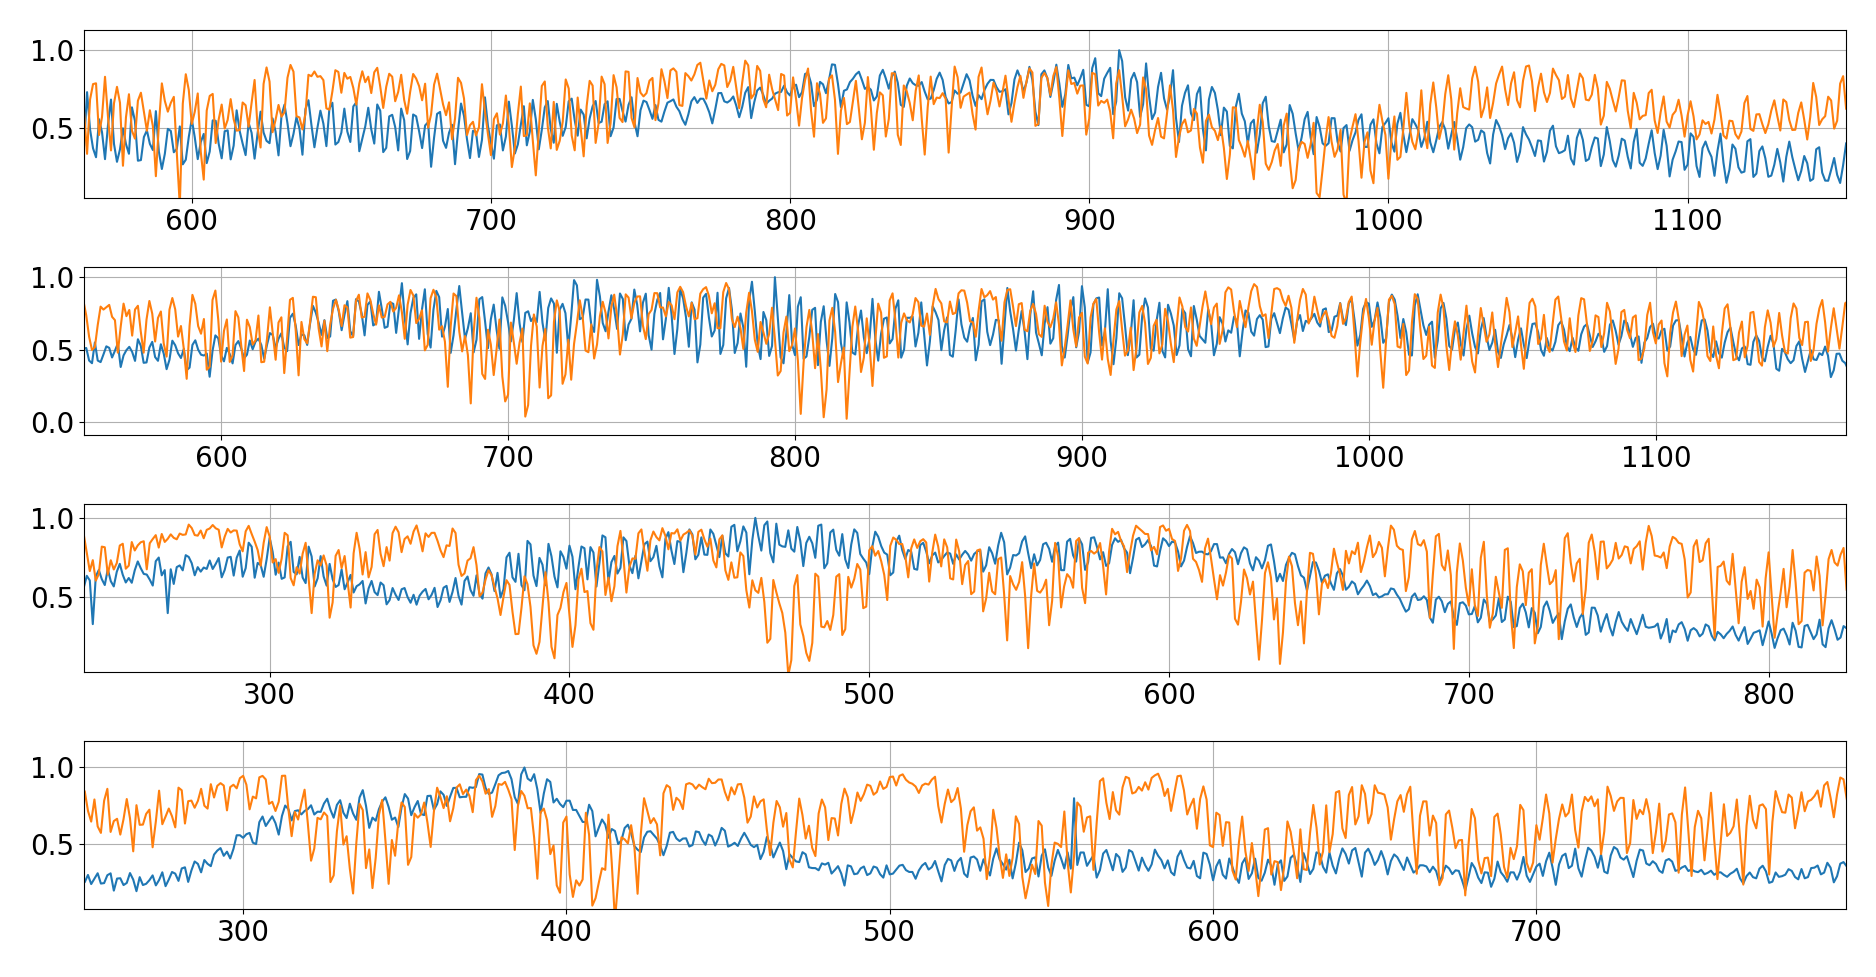
\includegraphics[width=\figwidth]{Figure_Chap4/20220811_P2VM_01_Flat1_1_Spectra_PolaOpposed.png}
    \caption[Graphiques comparant les wiggles observés sur les polarisations V et H sélectionnées par le prisme de wollaston, pour la puce $X$.]{Graphiques comparant les wiggles observés sur les polarisations V (en bleu) et H (en orange) sélectionnées par le prisme de wollaston. Les quatre graphiques tracent le flux des 4 sorties illuminées par l'entrée $1$ de la puce $X$.}
    \label{fig:WigglesInput1PolaComp}
\end{figure}

% Comparaison à l'oeil des wiggles entre les deux sorties de chaque base
Mais encore, la figure~\ref{fig:WigglesIniInjComp} montre le flux des deux sous-pupilles qui forment chacune des dix bases (dénommées sur les axes des ordonnées). Ainsi, on peut voir les \wiggles~formés sur les mêmes pixels de la caméra lorsqu'ils sont illuminés par l'une ou l'autre des entrées de la puce. Par exemple, le premier graphe trace le flux de la sortie $1$ lorsqu'elle est illuminée par l'entrée $1$ (en bleu) et par l'entrée $2$ (en orange). Ces deux sous-pupilles forment la base $1$. On voit, comme sur le graphique précédent, que les \wiggles~ne se superposent pas de manière consistante, ce qui élimine l'hypothèse qu'ils seraient formés par un effet de cavité Fabry-Pérot formée par les différentes couches constituant la caméra.

\begin{figure}[ht!]
    \centering
    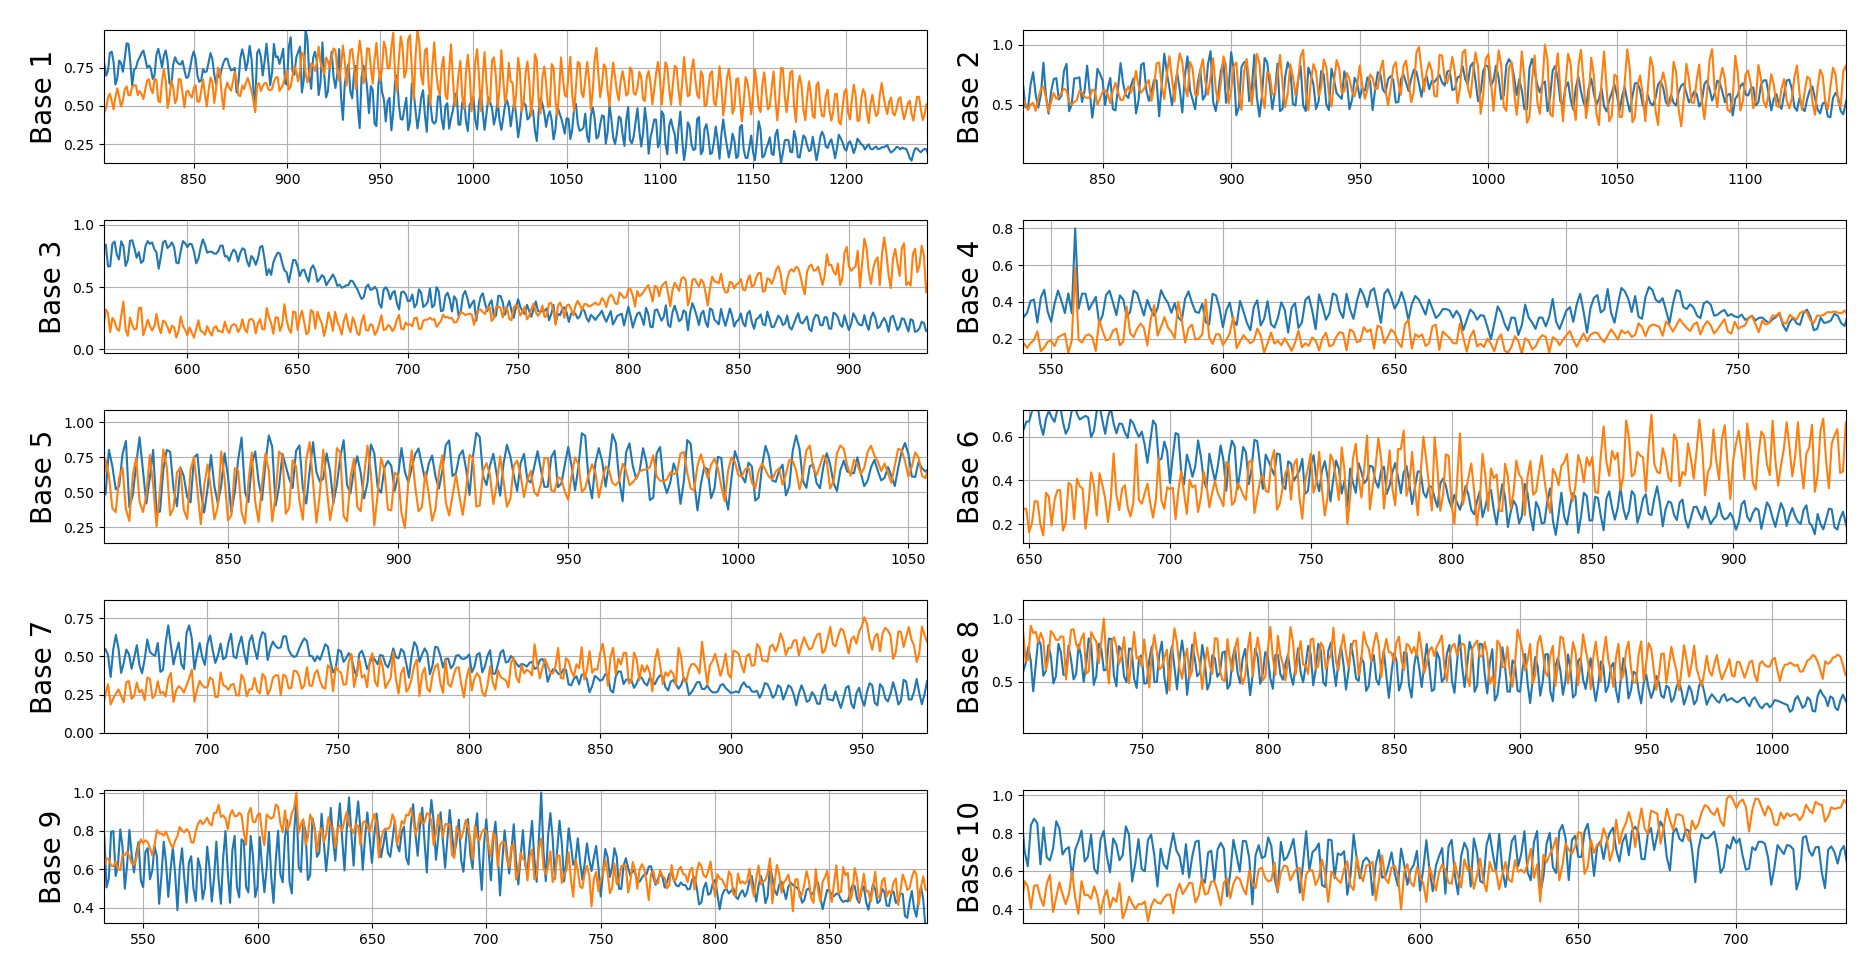
\includegraphics[width=\figwidth]{Figure_Chap4/20220811_P2VM_01_Flat1_Spectra_BaseOut1Out2_Pola1.png}
    \caption{}
    \label{fig:WigglesIniInjComp}
\end{figure}

% Contraste des wiggles
Ensuite, je souhaite calculer le contraste des \wiggles~à partir de l'équation du contraste des franges suivante :

\begin{equation}
    C = \frac{I_{max} - I_{min}}{I_{max} + I_{min}} \label{eq:FringeContrast}
\end{equation}

La figure~\ref{fig:WigglesContrast} présente cinq graphiques montrant à chaque fois les spectres (en noir) des quatre sorties illuminées, les spectres en polarisation V et en polarisation H étant dans la colonne de gauche et dans la colonne de droite, respectivement. Chaque spectre est encadré par deux courbes oranges $I_{max}$ et $I_{min}$ qui sont obtenues à partir de l'ajustement d'une fonction Spline, respectivement, sur les points maxima et sur les points minima du spectre. La courbe de contraste calculée à partir de l'équation~\ref{eq:FringeContrast} est tracée en rouge et la ligne horizontale en trait discontinu noir indique la valeur moyenne du contraste sur tous les canaux spectraux. La moyenne des contrastes mesurés sur toutes les sorties est de $\sim 0,16$ pour la polarisation V et de $\sim 0,37$ pour la polarisation H. On note que le contraste est plus d'un facteur deux plus grand sur la polarisation H que sur la polarisation V.

\begin{figure}[ht!]
    \centering
    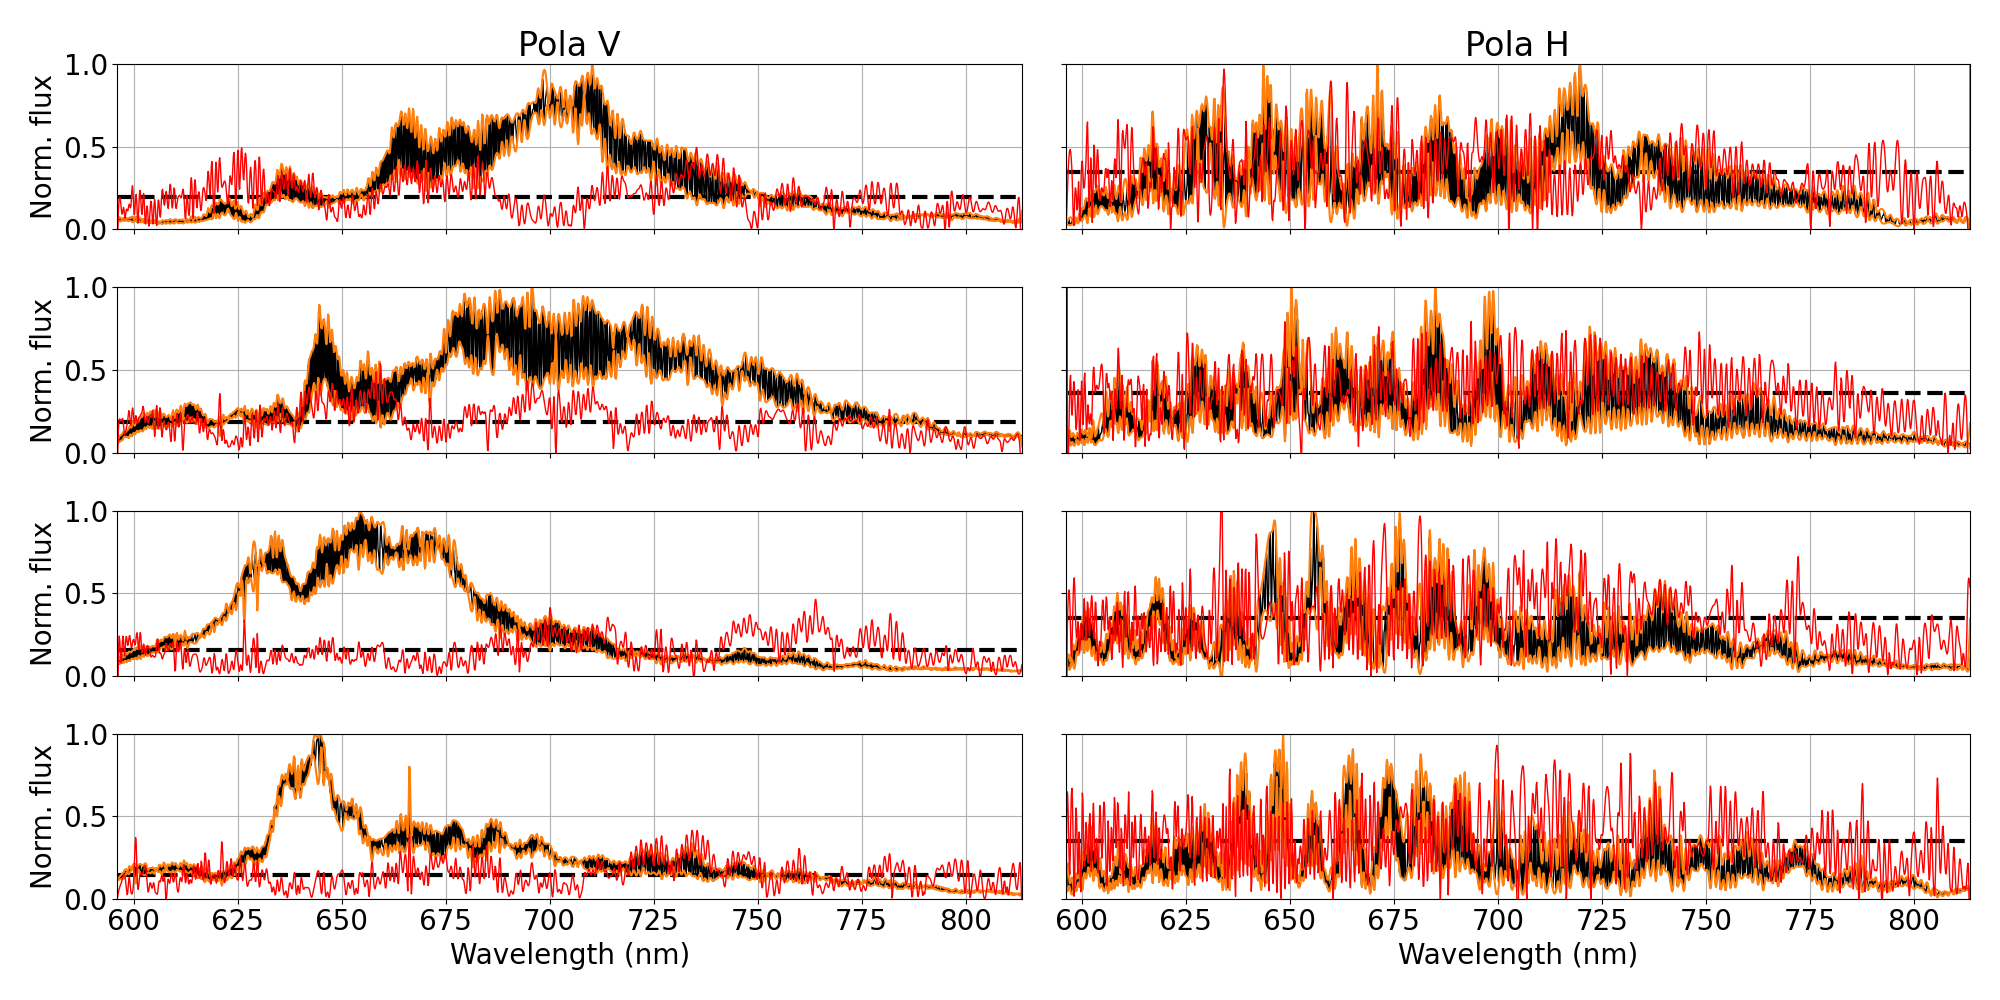
\includegraphics[width=\figwidth]{Figure_Chap4/20220811_P2VM_01_Flat1_1_WigglesContrast.png}
    \caption[]{}
    \label{fig:WigglesContrast}
\end{figure}

% FFT globale sur les flats
Afin d'étudier les propriétés fréquentielles des \wiggles, j'applique la transformé de Fourier sur les données précédemment présentées. La transformé de Fourier des quatre sorties (colonnes) illuminées successivement par les cinq entrées (lignes) de la puce est tracé sur la figure~\ref{fig:WigglesFFTGlobal} pour la polarisation V. Les couleurs entourant les graphiques indiquent les sorties illuminées sur les mêmes pixels de la caméra et dont leur combinaison forment une base (le code couleur est le même que sur les autres graphiques présentés tout au long de ce chapitre). On retrouve sur tous les graphiques les mêmes pics de fréquences : à $1.1 \,$nm$^{-1}$ et à $2 \,$nm$^{-1}$. Dans le cas de ce deuxième, il est parfois divisé en deux, trois ou quatre sous-pics. Les \wiggles, qui sont une modulation à haute fréquence, sont caractérisés par ce groupe de pics. De plus, on remarque que ces deux groupes de pics sont aussi présents sur les données en polarisation H.

\begin{figure}[ht!]
    \centering
    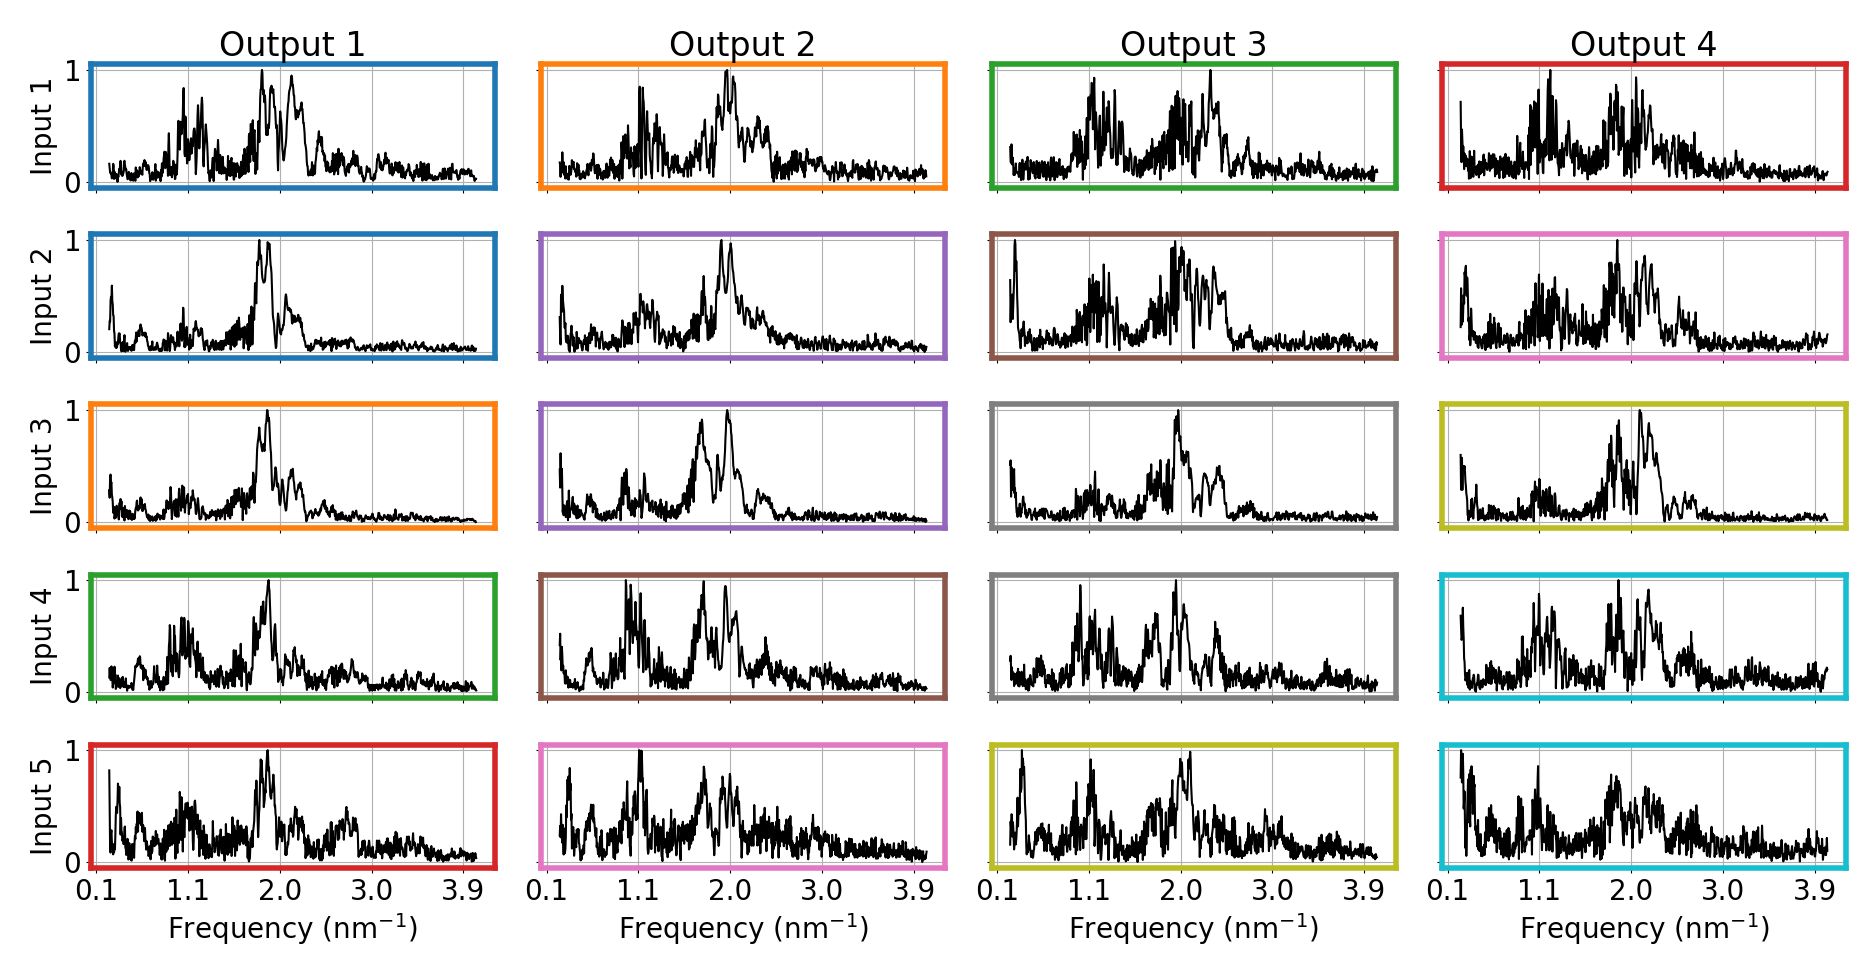
\includegraphics[width=\figwidth]{Figure_Chap4/20220811_P2VM_01_Flat1_InputOutput_Spectra_fft_Pola1.png}
    \caption[]{}
    \label{fig:WigglesFFTGlobal}
\end{figure}

% Présentation de la coupe en longueur d'onde des spectres pour faire une fft glissante
À présent, je souhaite étudier l'évolution de la fréquence des \wiggles~en fonction de la longueur d'onde. La figure~\ref{fig:WigglesSpectraCut} regroupe les tracés des quatre spectres par entrée illuminée (une entrée par ligne), en fonction de la longueur d'onde, pour la polarisation V. Ces spectres sont sectionnés en vingt sous-spectres sur lesquels j'appliquerai la transformé de Fourier (ce que je nommerai par la suite transformé de Fourier glissante). Chacun de ces sous-spectres sont démarqués par les barres verticales noires. On note que les spectres en polarisation H présentent des oscillations de basses fréquences, d'une dizaine de nanomètres de période environ, qui apparaissent avec une plus forte amplitude relative, en comparaison des spectres en polarisation V. Cette différence apparaît sur toutes les données avec un faible flux absolu. 

\begin{figure}[ht!]
    \centering
    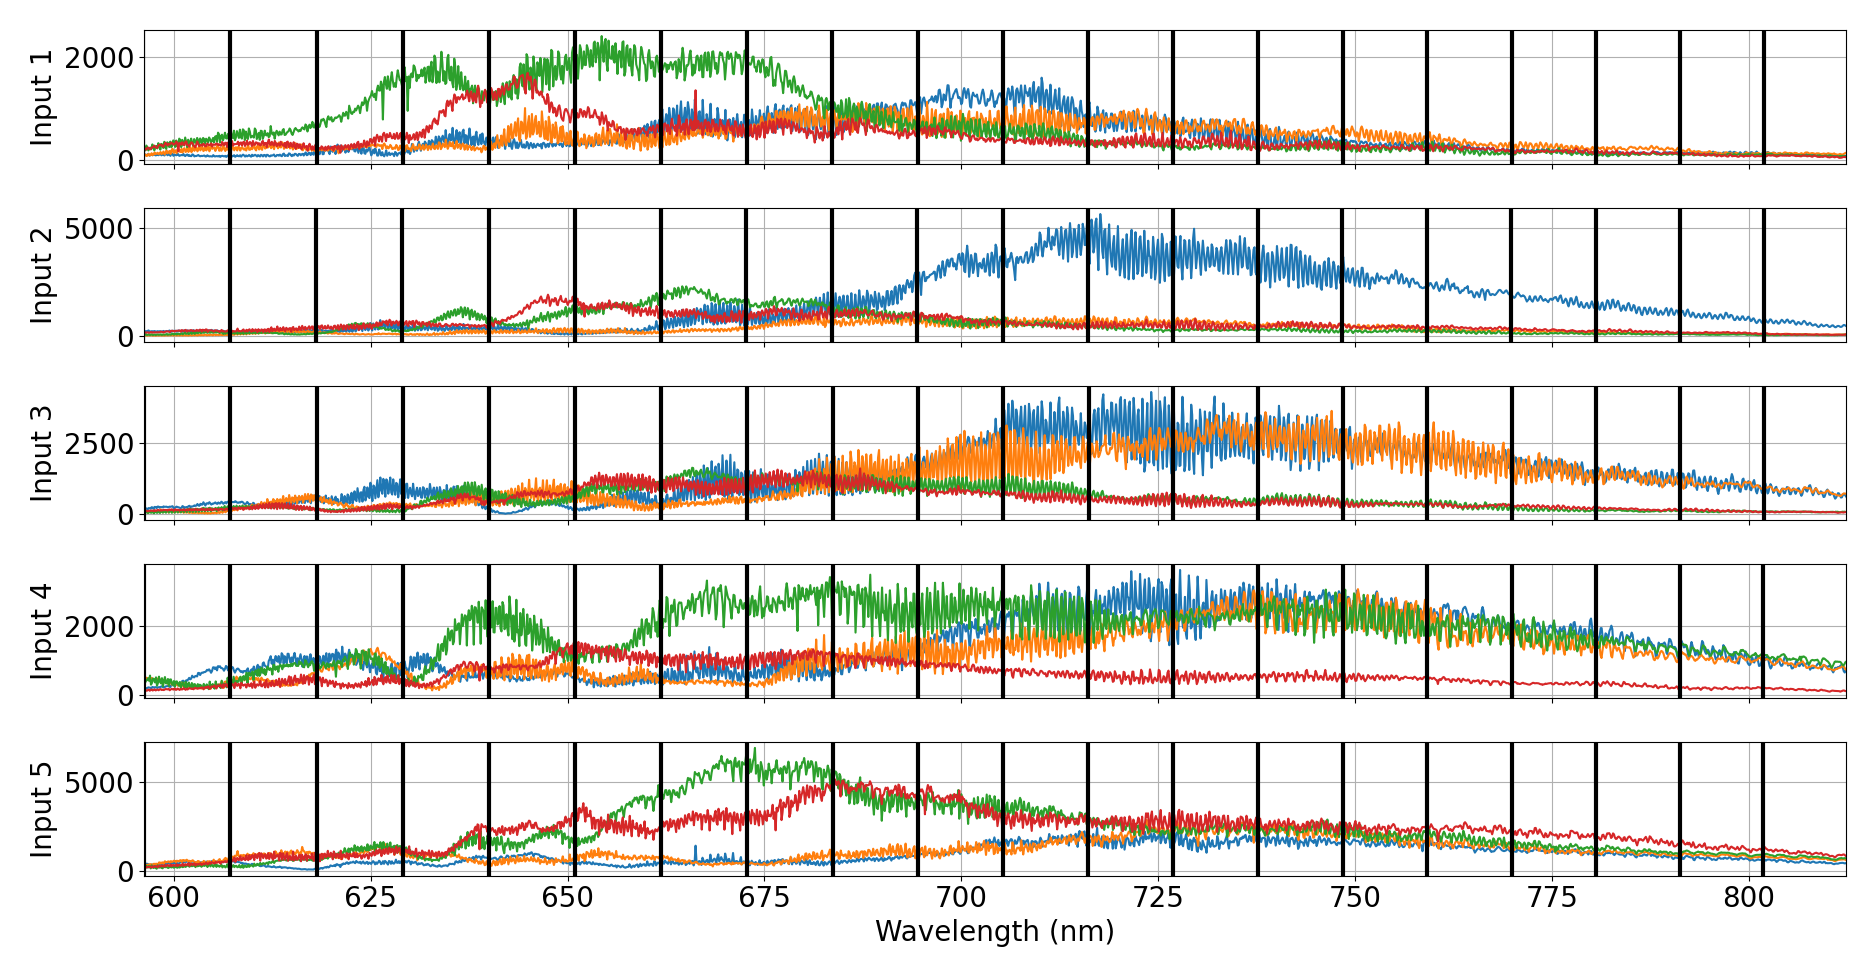
\includegraphics[width=\figwidth]{Figure_Chap4/20220811_P2VM_01_Flat1_SpectraCut_VS_Wave_Pola1_Base.png}
    \caption[]{}
    \label{fig:WigglesSpectraCut}
\end{figure}

% FFT glissante sur les spectres de tous les outputs
La figure~\ref{fig:WigglesFFTCut} montre les transformés de Fourier glissantes pour les quatre spectres obtenus (sur les colonnes) par l'illumination des cinq entrées (sur les lignes) de la puce pour la polarisation V. Les axes horizontaux sont les fréquences et les axes verticaux sont la longueur d'onde, prise au premier point de chaque section des spectres. On note que les transformés de Fourier présentent les mêmes caractéristiques quelle que soit la polarisation, de manière similaire à ce qu'on a pu voir sur les transformés de Fourier globales de la figure~\ref{fig:WigglesFFTGlobal}. Mais aussi, on remarque que les fréquences des pics diminuent avec la longueur d'onde, ce qui met en évidence que la période des \wiggles~augmente en fonction de la longueur d'onde.

\begin{figure}[ht!]
    \centering
    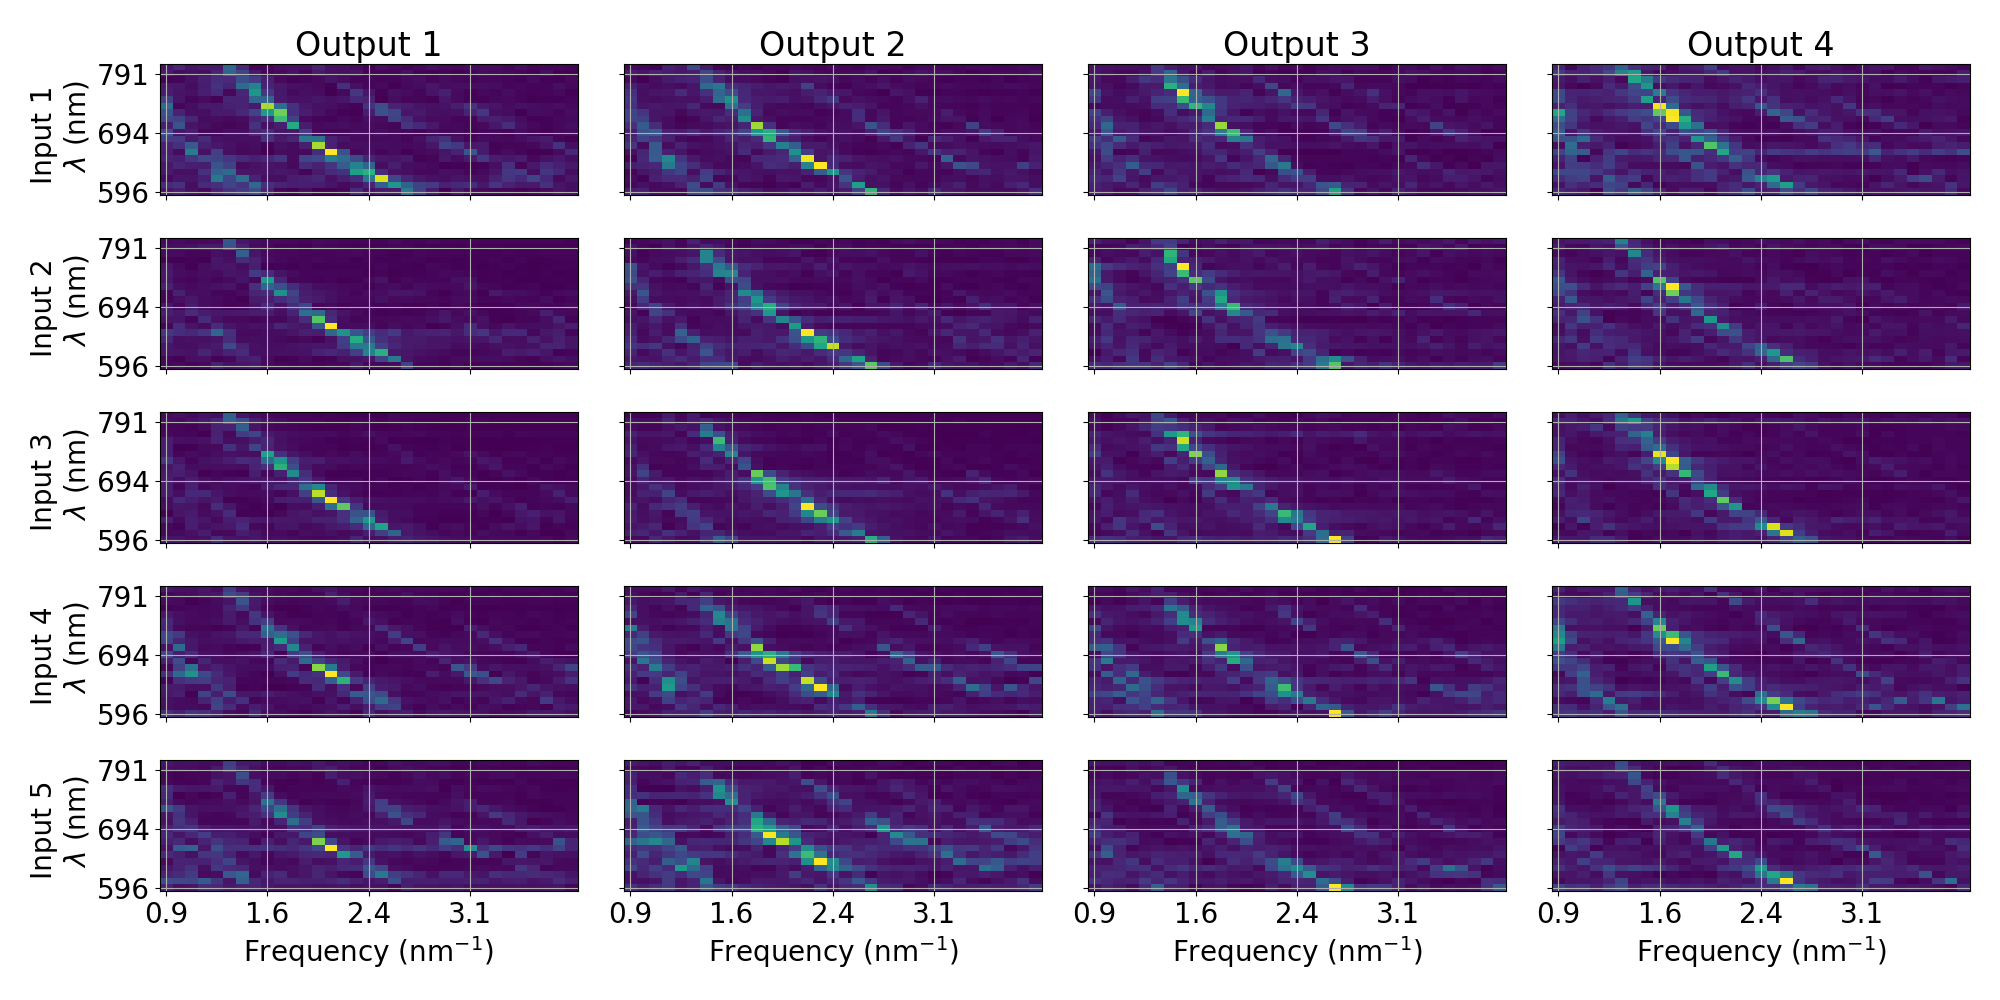
\includegraphics[width=\figwidth]{Figure_Chap4/20220811_P2VM_01_Flat1_InputOutput_Spectra_fft_VS_Wave_Pola1_Base.png}
    \caption[]{}
    \label{fig:WigglesFFTCut}
\end{figure}

% Fit du pic maximum de la fft
Afin de caractériser cette dépendance de la fréquence des \wiggles~en fonction de la longueur d'onde, j'effectue un ajustement du pic maximum des transformés de Fourier par une fonction polynomiale du second degré. Pour cela, la fréquence pour laquelle l'intensité est maximum sur les graphiques de la figure~\ref{fig:WigglesFFTCut} est sélectionné pour chaque longueur d'onde. La figure~\ref{fig:WigglesFitMaxFFTCut} montre cet ajustement pour toutes les transformés de Fourier et les coefficients polynomiaux trouvés sont indiqués dans les sous-titres. Le polynôme moyen qui ajuste les pic maxima de fréquence F s'écrit :

\begin{equation}
    \text{F} = (1,14.10^{-5} \pm 0,06.10^{-5}) \lambda^2 + (-2,18.10^{-2} \pm 0,09.10^{-2}) \lambda + 11,6 \pm 0,3
\end{equation}

Les coefficients polynomiaux sont les moyennes des coefficients ajustés pour tous les spectres ainsi que pour les deux polarisations car, comme on l'a vu précédemment, les transformés de Fourier sont les mêmes pour les deux polarisations et les fonctions ajustées sont similaires. Les incertitudes sont estimées à partir de l'écart-type sur l'ensemble des coefficients. Ainsi, les \wiggles~ont en moyenne une période de $\sim 0,5 \,$nm, ce qui correspond à environ $4 \,$px de la caméra.

\begin{figure}[ht!]
    \centering
    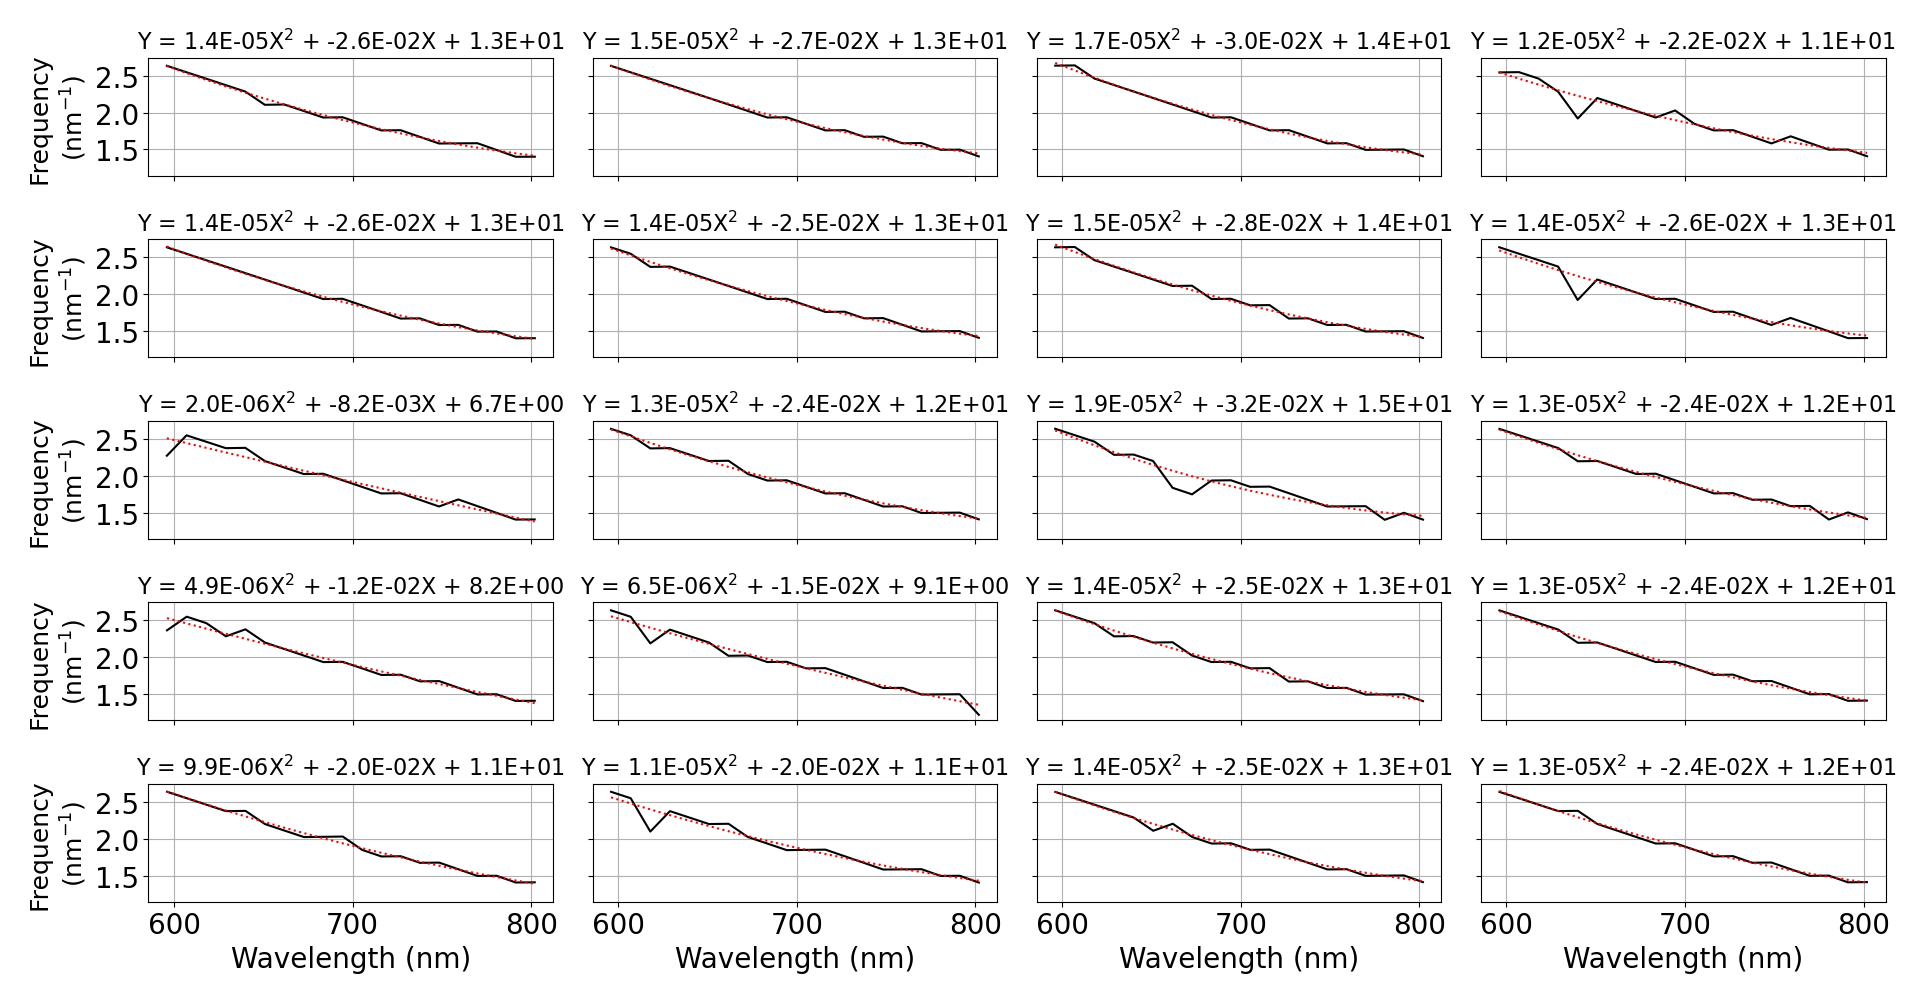
\includegraphics[width=\figwidth]{Figure_Chap4/20220811_P2VM_01_Flat1_InputOutput_Spectra_fftMaxFit_Pola1.png}
    \caption[]{}
    \label{fig:WigglesFitMaxFFTCut}
\end{figure}


%%%%%%%%%%%%%%%%
\subsection{Caractérisation des wiggles sur la puce Y}

Les résultats de cette étude sur les données prises avec la puce $Y$ sont similaire à ceux obtenus sur la puce $X$. De la même façon, les \wiggles~ne se superposent pas quelles que soient les sorties. Le contraste moyen des franges est mesuré à $\sim 0,14$ et l'équation polynomiale moyenne qui ajuste les pics maxima des transformés de Fourier en fonction de la longueur d'onde est :

\begin{equation}
    \text{F} = (1,48.10^{-5} \pm 0,06.10^{-5}) \lambda^2 + (-2,66.10^{-2} \pm 0,08.10^{-2}) \lambda + 13,3 \pm 0,3
\end{equation}

% Transformé de Fourier sur les phases différentielles
Les transformés de Fourier des phases différentielles brutes (de la figure~\ref{fig:PhaseDiffBinary} du haut) et des phases différentielles étalonnées (de la figure~\ref{fig:PhaseDiffBinary} du bas) pour les dix bases sont présentées sur la figure~\ref{fig:WigglesPhaseDiffA} et la figure~\ref{fig:WigglesPhaseDiffB}, respectivement. On note que l'étalonnage des phases différentielles n'induit pas de changement drastique sur les transformés de Fourier, cela efface seulement les pics de très basses fréquences, ce qui est le but recherché. On remarque la présence de trois (parfois quatre) pics principaux de fréquences sur les spectres qui sont situés aux mêmes fréquences que sur les mesures sur l'autre puce (autour de $4 \, \text{nm}^{-1}$). Il semble que ces pics ne se localisent pas aux mêmes fréquences et deux groupes semblent alors se démarquer.

\begin{figure}[ht!]
    \centering
    \begin{subfigure}{0.8\textwidth}
        \centering
        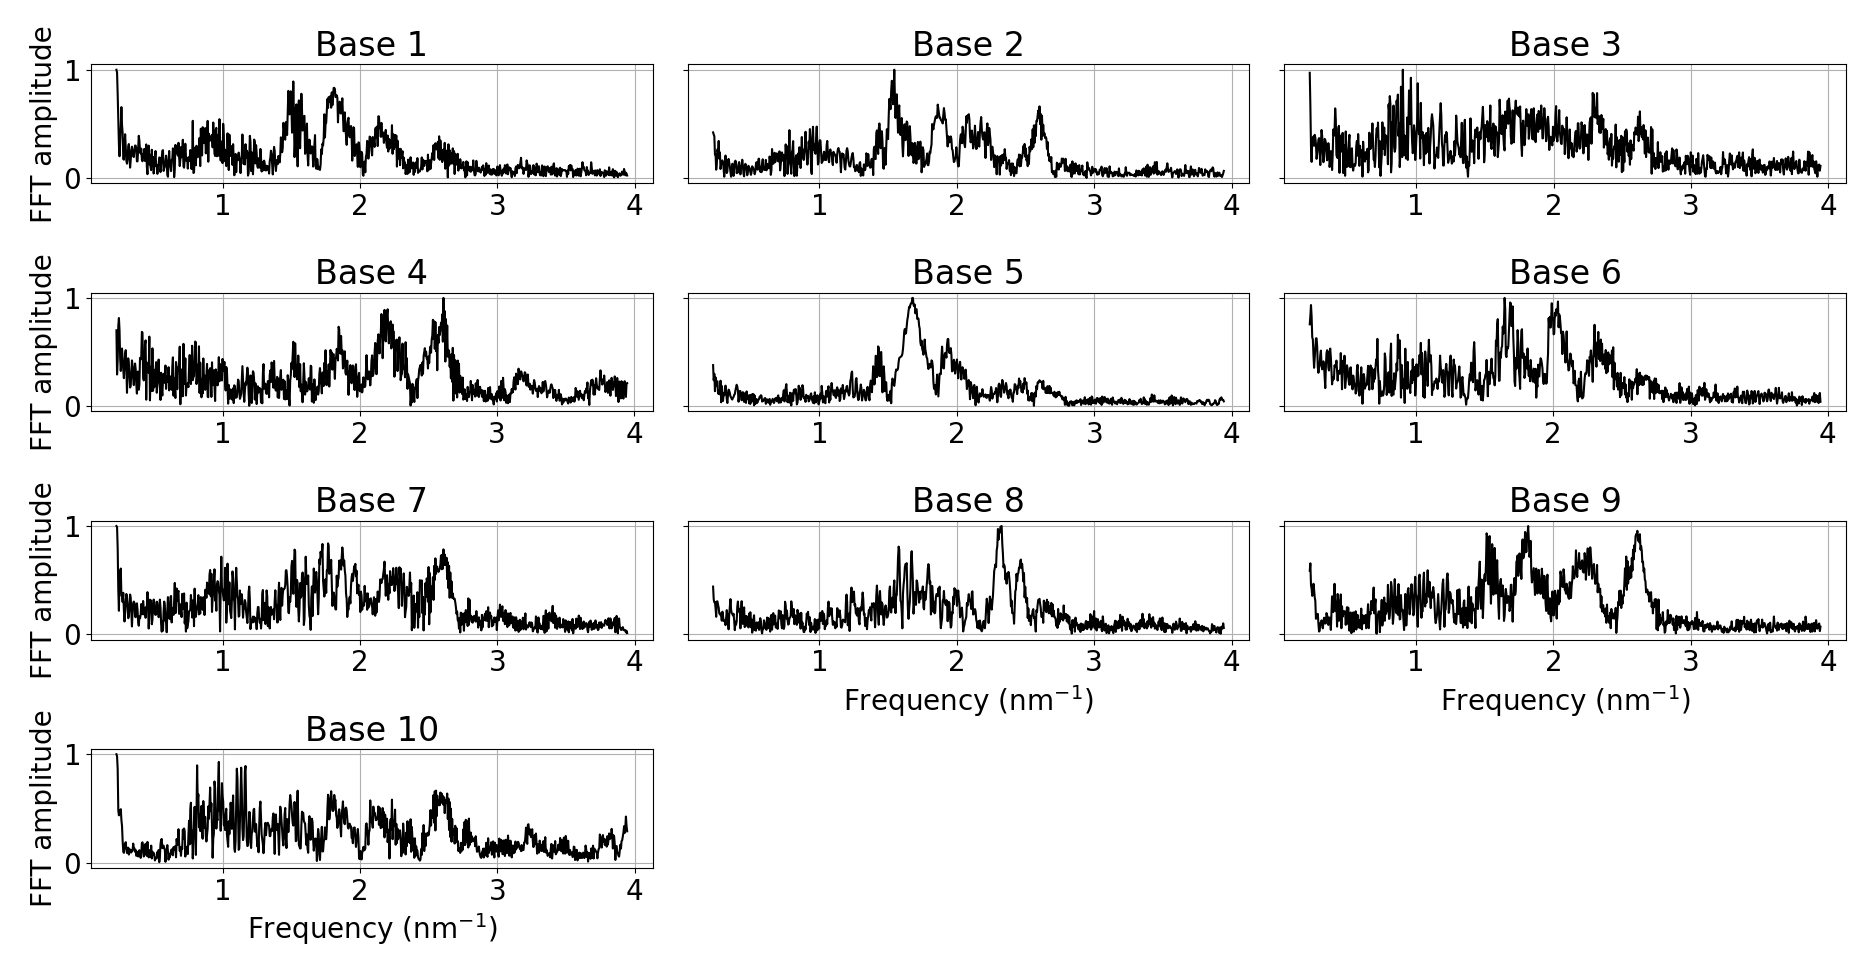
\includegraphics[width=\textwidth]{Figure_Chap4/20221010_Binary_01_Bin01_SpeDiffPhaseMean_fft_Pola1.png}
        \caption{}
        \label{fig:WigglesPhaseDiffA}
    \end{subfigure}
    \begin{subfigure}{0.8\textwidth}
        \centering
        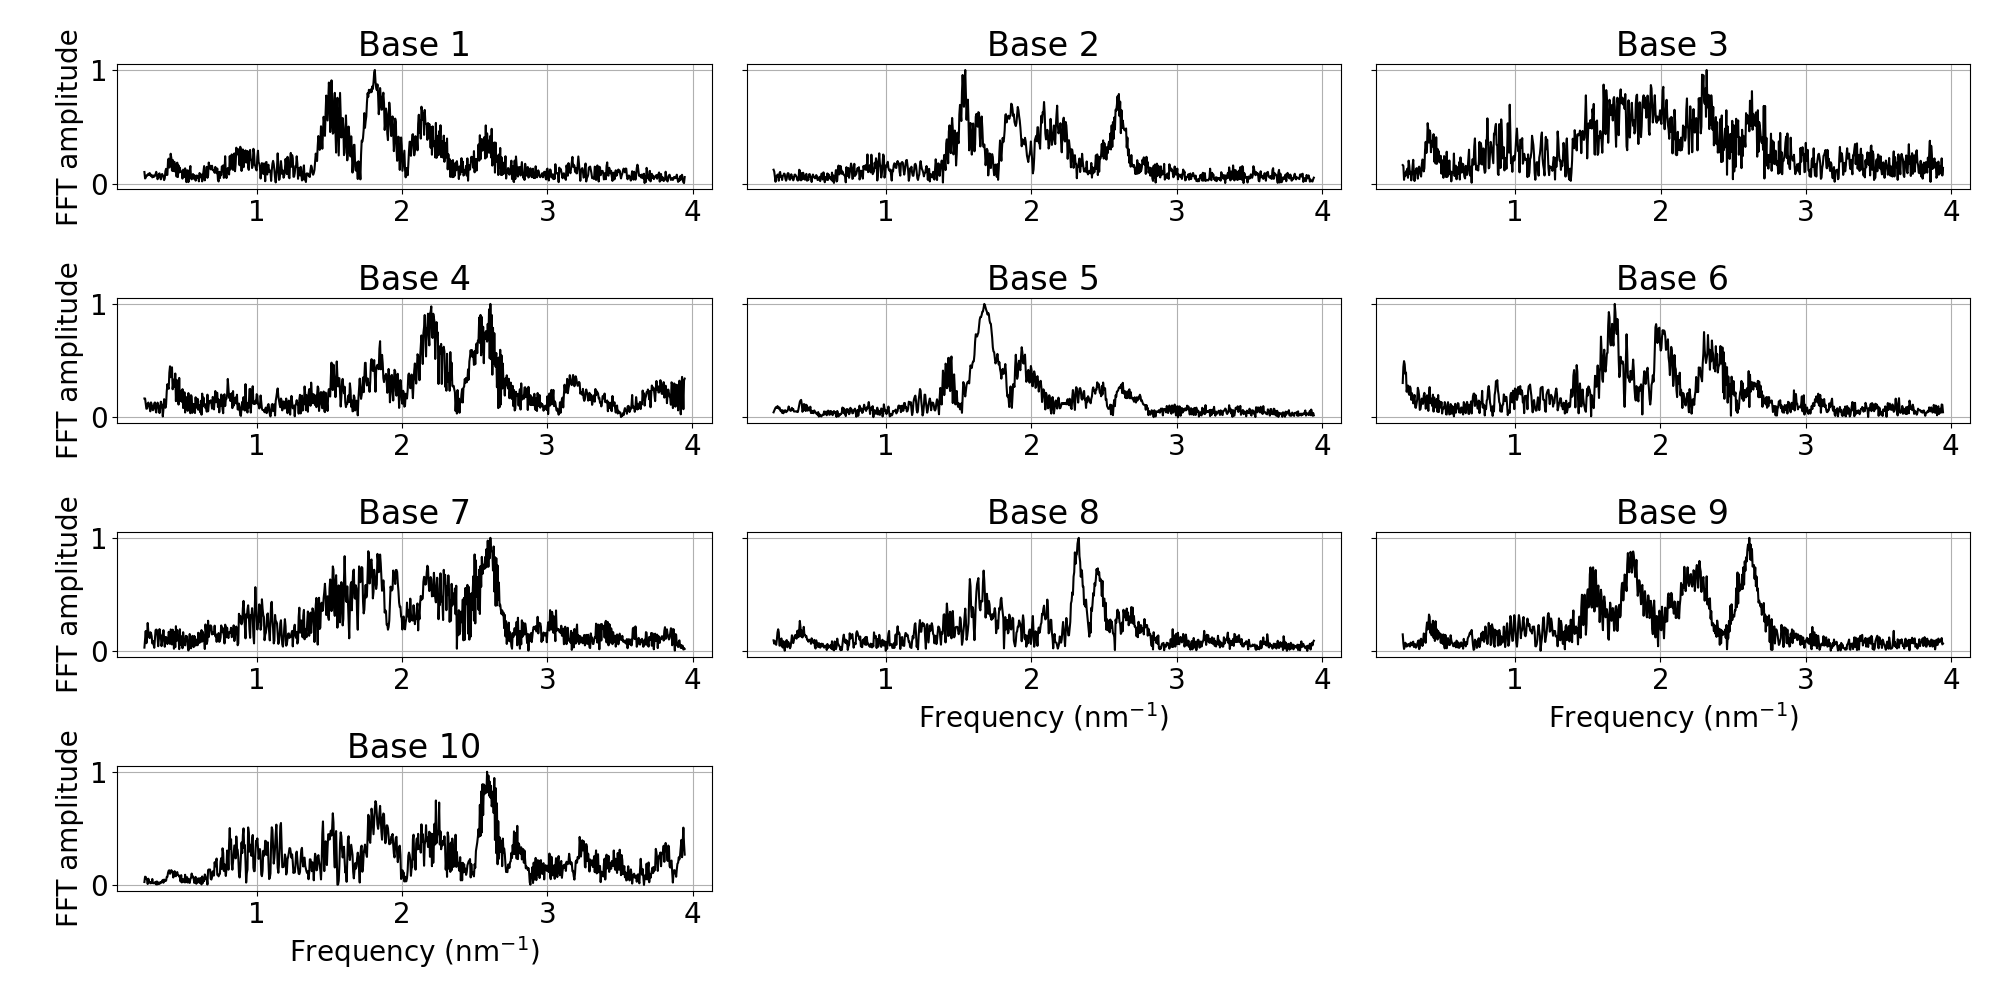
\includegraphics[width=\textwidth]{Figure_Chap4/20221010_Binary_01_Bin01_SpeDiffPhaseCal_fft_Pola1.png}
        \caption{}
        \label{fig:WigglesPhaseDiffB}
    \end{subfigure}
    \caption[]{}
    \label{fig:WigglesPhaseDiff}
\end{figure}

% Moyenne sur deux groupes de transformés de Fourier sélectionnés
En effet, la figure~\ref{fig:WigglesPhaseDiffMeanA} et la figure~\ref{fig:WigglesPhaseDiffMeanB} sont les transformés de Fourier moyennes sur deux groupes de bases (tracés en bleu et en rouge) pour les phases différentielles brutes et pour les phases différentielles étalonnées, respectivement. La forme des transformés de Fourier résultantes semblent comme en opposition de phases et reste inchangée après étalonnage des phases différentielles.

\begin{figure}[ht!]
    \centering
    \begin{subfigure}{0.8\textwidth}
        \centering
        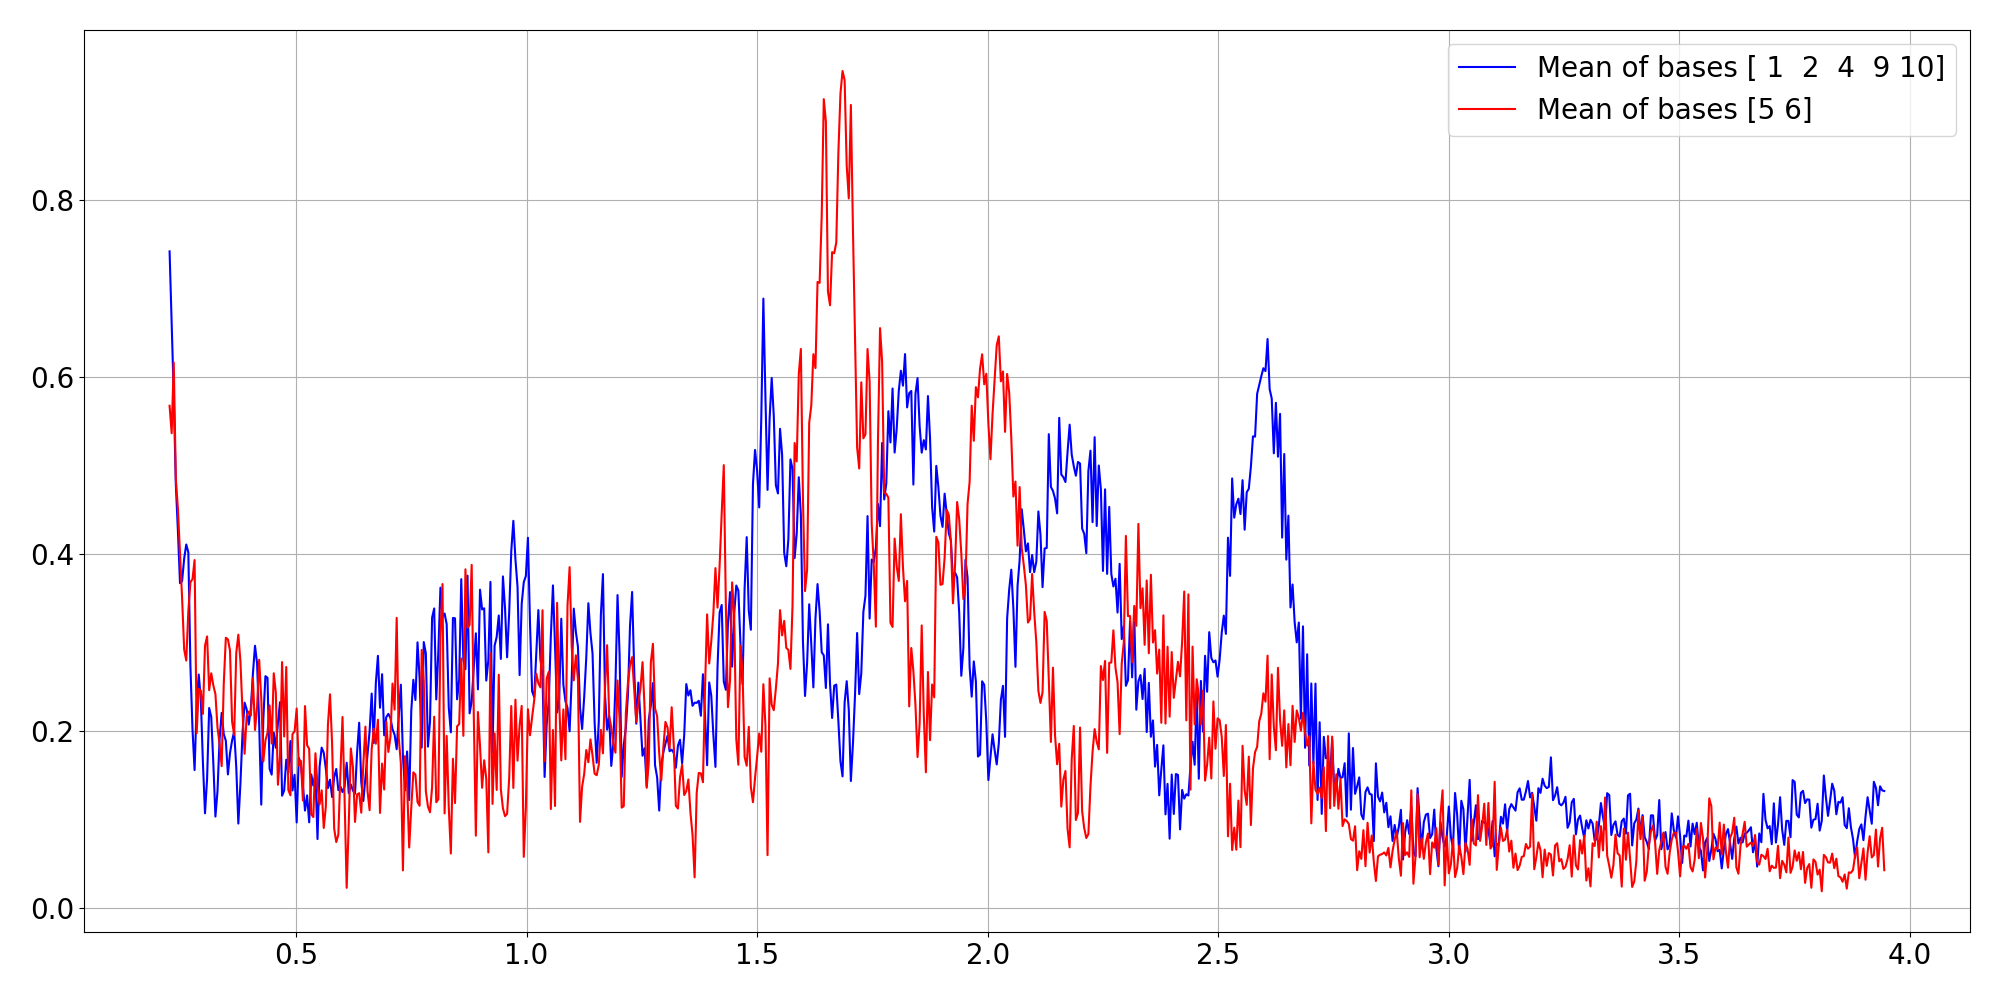
\includegraphics[width=\textwidth]{Figure_Chap4/20221010_Binary_01_Bin01_SpeDiffPhaseMean_fftBaseMean_Pola1.png}
        \caption{}
        \label{fig:WigglesPhaseDiffMeanA}
    \end{subfigure}
    \begin{subfigure}{0.8\textwidth}
        \centering
        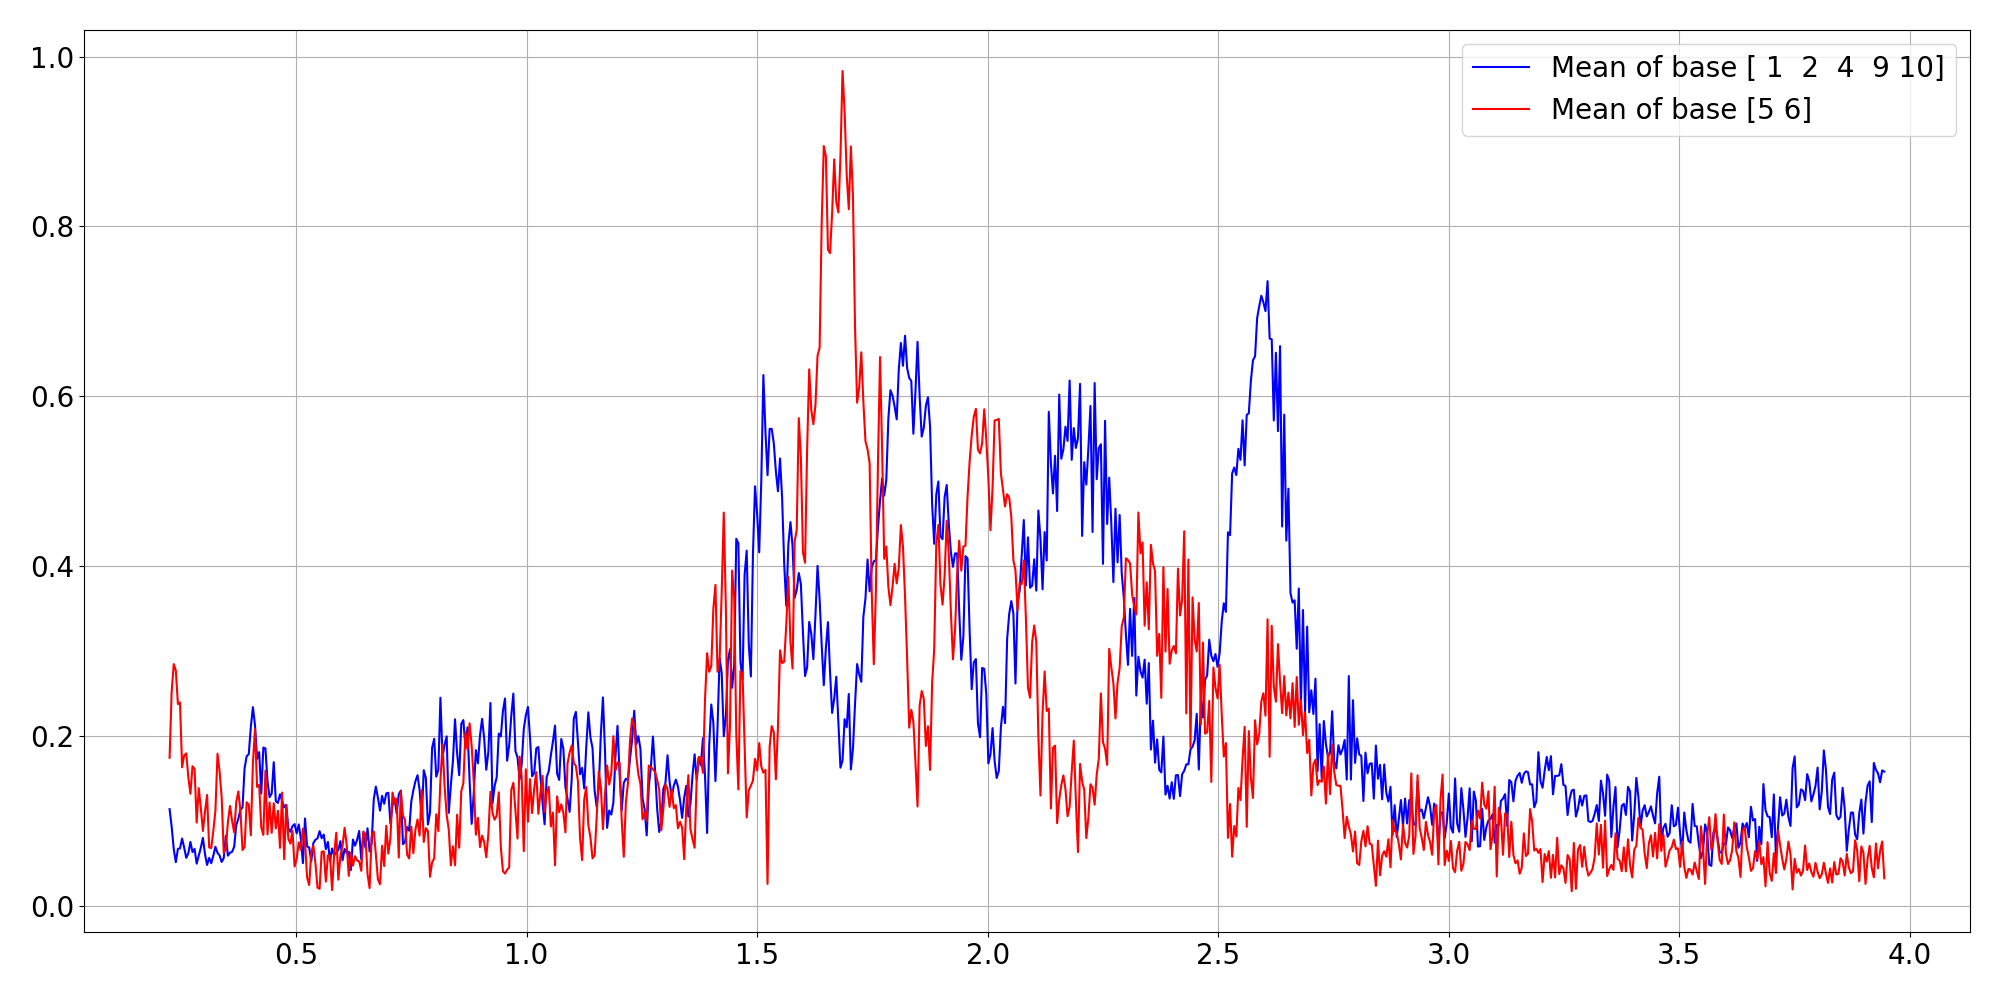
\includegraphics[width=\textwidth]{Figure_Chap4/20221010_Binary_01_Bin01_SpeDiffPhaseCal_fftBaseMean_Pola1.png}
        \caption{}
        \label{fig:WigglesPhaseDiffMeanB}
    \end{subfigure}
    \caption[]{}
    \label{fig:WigglesPhaseDiffMean}
\end{figure}


%%%%%%%%%%%%%%%%
\subsection{Les derniers tests en date sur le banc}

De récentes mesures effectuées sur le banc par Manon Lallement et Harry-Dean Kenchington Goldsmith semblent montrer que les puces ne sont pas à l'origine des \wiggles. Plusieurs tests ont été fait en injectant le faisceau à travers seulement une fibre qui illumine le spectrographe de \ac{FIRSTv2} :

\begin{itemize}
    \item en utilisant des polariseurs de différentes épaisseurs (avant ou après la fibre), la période des \wiggles~restent inchangée, ce qui montre qu'ils ne sont pas causés par une cavité Fabry-Pérot créée par le polariseur;
    \item en retirant le polariseur en entrée de fibre, les \wiggles~disparaissent;
    \item en utilisant un prisme de wollaston en entrée de fibre, les \wiggles~sont visibles.
\end{itemize}

Ainsi, il semblerait que la sélection d'une polarisation avant l'injection des faisceaux dans les fibres soit la cause de l'apparition de \wiggles. Or les puces ne sont pas à maintien de polarisation, c'est pour cela qu'on ne doit pas en injecter deux en entrée de la puce. De plus amples analyses sont nécessaires afin de déterminer une solution pour contourner ce problème.
\end{comment}
